\documentclass[../main.tex]{subfiles}
\begin{document}
	
The finite element method is a powerful tool for solving differential equations.
The method can easily deal with complex geometries and higher-order approximations of the solution. Figure \ref{fig:img_1} shows a two-dimensional domain with a non-trivial
geometry. The idea is to divide the domain into triangles (elements) and seek
a polynomial approximations to the unknown functions on each triangle. The
method glues these piecewise approximations together to find a global solution.
Linear and quadratic polynomials over the triangles are particularly popular.

\begin{figure}[H]
	\centering
	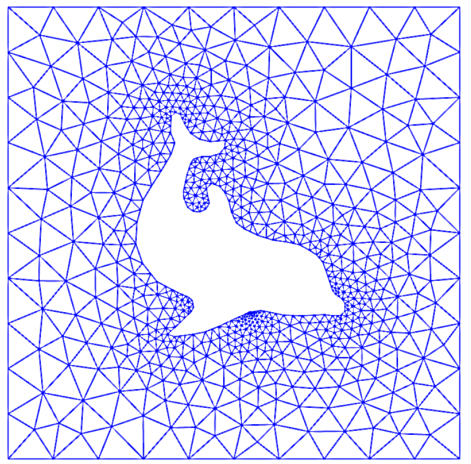
\includegraphics[width=0.7\linewidth]{img_1}
	\caption{Domain for flow around a dolphin.}
	\label{fig:img_1}
\end{figure}

Many successful numerical methods for differential equations, including the finite element method, aim at approximating the unknown function by a sum
\begin{equation}\label{eqa1}
	u(x)=\sum_{i=0}^{N} c_{i} \psi_{i}(x),
\end{equation}
where $\psi_{i}(x)$ are prescribed functions and $c_{0}, \ldots, c_{N}$ are unknown coefficients to be determined. Solution methods for differential equations utilizing (\ref{eqa1}) must have a \textit{principle} for constructing $N+1$ equations to determine $c_{0}, \ldots, c_{N}$. Then there is a \textit{machinery} regarding the actual constructions of the equations for $c_{0}, \ldots, c_{N}$, in a particular problem. Finally, there is a solve phase for computing the solution $c_{0}, \ldots, c_{N}$ of the $N+1$ equations.

Especially in the finite element method, the machinery for constructing the discrete equations to be implemented on a computer is quite comprehensive, with many mathematical and implementational details entering the scene at the same time. From an ease-of-learning perspective it can therefore be wise to introduce the computational machinery for a trivial equation: $u=f$. Solving this equation with $f$ given and $u$ on the form (\ref{eqa1}) means that we seek an approximation $u$ to $f$. This approximation problem has the advantage of introducing most of the finite element toolbox, but with postponing demanding topics related to differential equations (e.g., integration by parts, boundary conditions, and coordinate mappings). This is the reason why we shall first become familiar with finite element \textit{approximation} before addressing finite element methods for differential equations.

First, we refresh some linear algebra concepts about approximating vectors in vector spaces. Second, we extend these concepts to approximating functions in function spaces, using the same principles and the same notation. We present examples on approximating functions by global basis functions with support throughout the entire domain. Third, we introduce the finite element type of local basis functions and explain the computational algorithms for working with such functions. Three types of approximation principles are covered: 1) the least squares method, 2) the $L_{2}$ projection or Galerkin method, and 3 ) interpolation or collocation.
\chapter{Approximation of vectors}
\label{chap:chap_1}
\pagenumbering{arabic}
\setcounter{page}{1}
\noindent We shall start with introducing two fundamental methods for determining the
coefficients $c_{i}$
in (\ref{eqa1}) and illustrate the methods on approximation of vectors,
because vectors in vector spaces give a more intuitive understanding than starting
directly with approximation of functions in function spaces. The extension
from vectors to functions will be trivial as soon as the fundamental ideas are
understood.

The first method of approximation is called the \textit{least squares} method and
consists in finding $c_{i}$ such that the difference \textit{u} - \textit{f}, measured in some norm, is
minimized. That is, we aim at finding the best approximation \textit{u} to \textit{f} (in some
norm). The second method is not as intuitive: we find u such that the error
\textit{u} - \textit{f} is orthogonal to the space where we seek \textit{u}. This is known as \textit{projection},
or we may also call it a \textit{Galerkin method}. When approximating vectors and
functions, the two methods are equivalent, but this is no longer the case when
applying the principles to differential equations

\section[Approximation of planar vectors]{ Approximation of planar vectors}
\label{sec:sec_1_1}
\noindent Suppose we have given a vector \textit{\textbf{f}} = (3, 5) in the \textit{xy} plane and that we want to
approximate this vector by a vector aligned in the direction of the vector \textit{(a, b)}.
Figure \ref{fig:img_2} depicts the situation.

We introduce the vector space \textit{V} spanned by the vector $\psi_{0}$ = (a, b):

\begin{figure}[H]
	\centering
	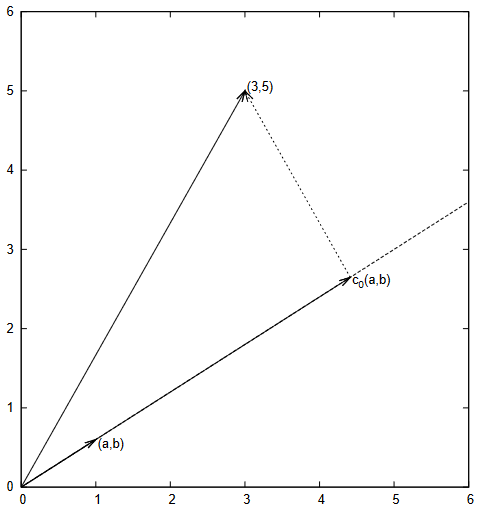
\includegraphics[width=0.7\linewidth]{img_2}
	\caption{Approximation of a two-dimensional vector by a one-dimensional vector.}
	\label{fig:img_2}
\end{figure}
\begin{equation}\label{eqa2}
	V=\operatorname{span}\left\{\psi_{0}\right\}
\end{equation}

\noindent We say that $\psi_{0}$ is a basis vector in the space $V$. Our aim is to find the vector $\boldsymbol{u}=c_{0} \psi_{0} \in V$ which best approximates the given vector $\boldsymbol{f}=(3,5)$. A reasonable criterion for a best approximation could be to minimize the length of the difference between the approximate u and the given $\boldsymbol{f}$. The difference, or error $e=\boldsymbol{f}-\boldsymbol{u}$, has its length given by the \textit{norm}
$$
	\|e\|=(e, e)^{\frac{1}{2}},
$$
where $(e, e)$ is the \textit{inner product} of $e$ and itself. The inner product, also called \textit{scalar product} or \textit{dot product}, of two vectors $\boldsymbol{u}=\left(u_{0}, u_{1}\right)$ and $\boldsymbol{v}=\left(v_{0}, v_{1}\right)$ is defined as
\begin{equation}\label{eqa3}
	(\boldsymbol{u}, \boldsymbol{v})=u_{0} v_{0}+u_{1} v_{1}.
\end{equation}

\noindent \textbf{Remark 1.} We should point out that we use the notation $(\cdot, \cdot)$ for two different things: $(a, b)$ for scalar quantities $a$ and $b$ means the vector starting in the origin and ending in the point $(a, b)$, while $(\boldsymbol{u}, \boldsymbol{v})$ with vectors $\boldsymbol{u}$ and $\boldsymbol{v}$ means the inner product of these vectors. Since vectors are here written in boldface font there should be no confusion. We may add that the norm associated with this inner product is the usual Eucledian length of a vector.
\bigbreak
\noindent \textbf{Remark 2.} It might be wise to refresh some basic linear algebra by consulting a textbook. Exercises \hyperref[sec:sec_10_1]{1} and \hyperref[sec:sec_10_1]{2} suggest specific tasks to regain familiarity with fundamental operations on inner product vector spaces.
\bigbreak
\noindent \textbf{The least squares method}. We now want to find $c_{0}$ such that it minimizes $\|e\|$. The algebra is simplified if we minimize the square of the norm, $\|e\|^{2}=$ $(e, e)$, instead of the norm itself. Define the function
\begin{equation}\label{eqa4}
	E\left(c_{0}\right)=(e, e)=\left(\boldsymbol{f}-c_{0} \psi_{0}, \boldsymbol{f}-c_{0} \psi_{0}\right).
\end{equation}
We can rewrite the expressions of the right-hand side in a more convenient form for further work:
\begin{equation}\label{eqa5}
	E\left(c_{0}\right)=(\boldsymbol{f}, \boldsymbol{f})-2 c_{0}\left(\boldsymbol{f}, \psi_{0}\right)+c_{0}^{2}\left(\psi_{0}, \psi_{0}\right).
\end{equation}
The rewrite results from using the following fundamental rules for inner product spaces:

\begin{equation}\label{eqa6}
	(\alpha u, v)=\alpha(u, v), \quad \alpha \in \mathbb{R},
\end{equation}
\begin{equation}\label{eqa7}
	(u + v, w)=(u, w)+(v, w),
\end{equation}
\begin{equation}\label{eqa8}
	(u, v)= (v, u)
\end{equation}
\indent Minimizing $E\left(c_{0}\right)$ implies finding $c_{0}$ such that
$$
\frac{\partial E}{\partial c_{0}}=0.
$$
Differentiating (\ref{eqa5}) with respect to $c_{0}$ gives
\begin{equation}\label{eqa9}
	\frac{\partial E}{\partial c_{0}}=-2\left(\boldsymbol{f}, \psi_{0}\right)+2 c_{0}\left(\psi_{0}, \psi_{0}\right)
\end{equation}
Setting the above expression equal to zero and solving for $c_{0}$ gives
\begin{equation}\label{eqa10}
	c_{0}=\frac{\left(\boldsymbol{f}, \psi_{0}\right)}{\left(\psi_{0}, \psi_{0}\right)}
\end{equation}
which in the present case with $\psi_{0}=(a, b)$ results in
\begin{equation}\label{eqa11}
	c_{0}=\frac{3 a+5 b}{a^{2}+b^{2}}.
\end{equation}
For later, it is worth mentioning that setting the key equation (\hyperref[eqa9]{9}) to zero can be rewritten as
$$
\left(f-c 0 \psi_{0}, \psi_{0}\right)=0,
$$
or
\begin{equation}\label{eqa12}
	\left(e, \psi_{0}\right)=0.
\end{equation}
\textbf{The projection method.} We shall now show that minimizing $\|e\|^{2}$ implies that $\boldsymbol{e}$ is orthogonal to \textit{any} vector $\boldsymbol{v}$ in the space $V$. This result is visually quite clear from Figure \hyperref[fig:img_2]{2} (think of other vectors along the line $(a, b)$ : all of them will lead to a larger distance between the approximation and $\boldsymbol{f})$. To see this result mathematically, we express any $v \in V$ as $v=s \psi_{0}$ for any scalar parameter $s$, recall that two vectors are orthogonal when their inner product vanishes, and calculate the inner product
$$
\begin{aligned}
	\left(e, s \psi_{0}\right) &=\left(\boldsymbol{f}-c_{0} \psi_{0}, s \psi_{0}\right) \\
	&=\left(\boldsymbol{f}, s \psi_{0}\right)-\left(c_{0} \psi_{0}, s \psi_{0}\right) \\
	&=s\left(\boldsymbol{f}, \psi_{0}\right)-s c_{0}\left(\psi_{0}, \psi_{0}\right) \\
	&=s\left(\boldsymbol{f}, \psi_{0}\right)-s \frac{\left(\boldsymbol{f}, \psi_{0}\right)}{\left(\psi_{0}, \psi_{0}\right)}\left(\psi_{0}, \psi_{0}\right) \\
	&=s\left(\left(\boldsymbol{f}, \psi_{0}\right)-\left(\boldsymbol{f}, \psi_{0}\right)\right) \\
	&=0 .
\end{aligned}
$$
Therefore, instead of minimizing the square of the norm, we could demand that $\boldsymbol{e}$ is orthogonal to any vector in $V$. This method is known as \textit{projection}, because it is the same as projecting the vector onto the subspace. (The approach can also be referred to as a Galerkin method as explained at the end of Section ??.)
Mathematically the projection method is stated by the equation
\begin{equation}\label{eqa13}
	(e, v)=0, \quad \forall v \in V.
\end{equation}
An arbitrary $\boldsymbol{v} \in V$ can be expressed as $s \psi_{0}, s \in \mathbb{R}$, and therefore (\hyperref[eqa13]{13}) implies
$$
\left(e, s \psi_{0}\right)=s\left(e, \psi_{0}\right)=0
$$
which means that the error must be orthogonal to the basis vector in the space $V$ :
$$
\left(e, \psi_{0}\right)=0 \quad \text { or } \quad\left(f-c_{0} \psi_{0}, \psi_{0}\right)=0.
$$
The latter equation gives (10) and it also arose from least squares computations in (\hyperref[eqa12]{12}).

\section[Approximation of general vectors]{Approximation of general vectors}
\label{sec:sec_1_2}
\noindent Let us gencralize the vector approximation from the previous section to vectors in spaces with arbitrary dimension. Given some vector $\boldsymbol{f}$, we want to find the best approximation to this vector in the space
$$
V=\operatorname{span}\left\{\psi_{0}, \ldots, \psi_{N}\right\}.
$$
We assume that the \textit{basis vectors} $\psi_{0}, \ldots, \psi_{N}$ are linearly independent so that none of them are redundant and the space has dimension $N+1$. Any vector $\boldsymbol{u} \in V$ can be written as a linear combination of the basis vectors,
$$
\boldsymbol{u}=\sum_{j=0}^{N} c_{j} \psi_{j},
$$
where $c_{j} \in \mathbb{R}$ are scalar coefficients to be determined.
\bigbreak
\noindent \textbf{The least squares method.} Now we want to find $c_{0}, \ldots, c_{N}$, such that u is the best approximation to $\boldsymbol{f}$ in the sense that the distance (error) $e=\boldsymbol{f}-u$ is minimized. Again, we define the squared distance as a function of the free parameters $c_{0}, \ldots, c_{N}$,
\begin{equation}\label{eqa14}
	\begin{aligned}
	E\left(c_{0}, \ldots, c_{N}\right) &=(e, e)=\left(\boldsymbol{f}-\sum_{j} c_{j} \psi_{j}, \boldsymbol{f}-\sum_{j} c_{j} \psi_{j}\right) \\
	&=(\boldsymbol{f}, \boldsymbol{f})-2 \sum_{j=0}^{N} c_{j}\left(\boldsymbol{f}, \psi_{j}\right)+\sum_{p=0}^{N} \sum_{q=0}^{N} c_{p} c_{q}\left(\psi_{p}, \psi_{q}\right)
	\end{aligned}
\end{equation}
Minimizing this $E$ with respect to the independent variables $c_{0}, \ldots, c_{N}$ is obtained by requiring
$$
\frac{\partial E}{\partial c_{i}}=0, \quad i=0, \ldots, N
$$
The second term in (\hyperref[eqa14]{14}) is differentiated as follows:
\begin{equation}\label{eqa15}
	\frac{\partial}{\partial c_{i}} \sum_{j=0}^{N} c_{j}\left(\boldsymbol{f}, \psi_{j}\right)=\left(\boldsymbol{f}, \psi_{i}\right),
\end{equation}
since the expression to be differentiated is a sum and only one term, $c_{i}\left(\boldsymbol{f}, \psi_{i}\right)$, contains $c_{i}$ and this term is linear in $c_{i}$. To understand this differentiation in detail, write out the sum specifically for, e.g, $N=3$ and $i=1$.

The last term in (\hyperref[eqa14]{14}) is more tedious to differentiate. We start with
\begin{equation}\label{eqa16}
	\frac{\partial}{\partial c_{i}} c_{p} c_{q}= \begin{cases}0, & \text { if } p \neq i \text { and } q \neq i, \\ c_{q}, & \text { if } p=i \text { and } q \neq i \\ c_{p}, & \text { if } p \neq i \text { and } q=i, \\ 2 c_{i}, & \text { if } p=q=i,\end{cases}
\end{equation}
Then
$$
\frac{\partial}{\partial c_{i}} \sum_{p=0}^{N} \sum_{q=0}^{N} c_{p} c_{q}\left(\psi_{p}, \psi_{q}\right)=\sum_{p=0, p \neq i}^{N} c_{p}\left(\psi_{p}, \psi_{i}\right)+\sum_{q=0, q \neq i}^{N} c_{q}\left(\psi_{q}, \psi_{i}\right)+2 c_{i}\left(\psi_{i}, \psi_{i}\right).
$$
The last term can be included in the other two sums, resulting in
\begin{equation}\label{eqa17}
	\frac{\partial}{\partial c_{i}} \sum_{p=0}^{N} \sum_{q=0}^{N} c_{p} c_{q}\left(\psi_{p}, \psi_{q}\right)=2 \sum_{j=0}^{N} c_{i}\left(\psi_{j}, \psi_{i}\right).
\end{equation}
It then follows that setting
\begin{equation}\label{eqa18}
\frac{\partial E}{\partial c_{i}}=0, \quad i=0, \ldots, N,
$$
leads to a linear system for $c_{0}, \ldots, c_{N}$ :
$$
\sum_{j=0}^{N} A_{i, j} c_{j}=b_{i}, \quad i=0, \ldots, N,
\end{equation}	
where
\begin{equation}\label{eqa19}
	\begin{aligned}
	A_{i, j} &=\left(\psi_{i}, \psi_{j}\right),
	\end{aligned}
\end{equation}
\begin{equation}\label{eqa20}
	\begin{aligned}
	b_{i} &=\left(\psi_{i}, \boldsymbol{f}\right).
	\end{aligned}
\end{equation}
We have changed the order of the two vectors in the inner product according to (\hyperref[sec:sec_1_1]{1.1}):
$$
A_{i, j}=\left(\psi_{j}, \psi_{i}\right)=\left(\psi_{i}, \psi_{j}\right),
$$
simply because the sequence $i$ - $j$ looks more aesthetic.
\bigbreak
\noindent \textbf{The Galerkin or projection method.} In analogy with the "one-dimensional" example in Section \hyperref[sec:sec_1_1]{1.1}, it holds also here in the general case that minimizing the distance (error) $\boldsymbol{e}$ is equivalent to demanding that $\boldsymbol{e}$ is orthogonal to all $\boldsymbol{v} \in V$ :
\begin{equation}\label{eqa21}
	(e, v)=0, \quad \forall v \in V.
\end{equation}
Since any $\boldsymbol{v} \in V$ can be written as $\boldsymbol{v}=\sum_{i=0}^{N} c_{i} \psi_{i}$, the statement (\hyperref[eqa21]{21}) is equivalent to saying that
$$
\left(e, \sum_{i=0}^{N} c_{i} \psi_{i}\right)=0,
$$
for any choice of coefficients $c_{0}, \ldots, c_{N}$. The latter equation can be rewritten as

$$
\sum_{i=0}^{N} c_{i}\left(e, \psi_{i}\right)=0.
$$
If this is to hold for arbitrary values of $c_{0}, \ldots, c_{N}$ we must require that each term in the sum vanishes,
\begin{equation}\label{eqa22}
	\left(e, \psi_{i}\right)=0, \quad i=0, \ldots, N.
\end{equation}
These $N+1$ equations result in the same linear system as (\hyperref[eqa18]{18}):
$$
\left(\boldsymbol{f}-\sum_{j=0}^{N} c_{j} \psi_{j}, \psi_{i}\right)=\left(\boldsymbol{f}, \psi_{i}\right)-\sum_{j \in \mathcal{I}_{\mathrm{a}}}\left(\psi_{i}, \psi_{j}\right) c_{j}=0,
$$
and hence
$$
\sum_{j=0}^{N}\left(\psi_{i}, \psi_{j}\right) c_{j}=\left(\boldsymbol{f}, \psi_{i}\right), \quad i=0, \ldots, N.
$$
So, instead of differentiating the $E\left(c_{0}, \ldots, c_{N}\right)$ function, we could simply use (\hyperref[eqa21]{21}) as the principle for determining $c_{0}, \ldots, c_{N}$, resulting in the $N+1$ equations (\hyperref[eqa22]{22}).

The names \textit{least squares method} or \textit{least squares approximation} are natural since the calculations consists of minimizing $\|e\|^{2}$, and $\|e\|^{2}$ is a sum of squares of differences between the components in $\boldsymbol{f}$ and $\boldsymbol{u}$. We find $\boldsymbol{u}$ such that this sum of squares is minimized.

The principle (\hyperref[eqa21]{21}), or the equivalent form (\hyperref[eqa22]{22}), is known as projection. Almost the same mathematical idea was used by the Russian mathematician \href{https://en.wikipedia.org/wiki/Boris_Galerkin}{Boris Galerkin} to solve differential equations, resulting in what is widely known as \textit{Galerkin's method.}

\chapter{Approximation of functions}
\label{chap:chap_2}
Let $V$ be a function space spanned by a set of \textit{basis functions} $\psi_{0}, \ldots, \psi_{N}$,
$$
V=\operatorname{span}\left\{\psi_{0}, \ldots, \psi_{N}\right\},
$$
such that any function $u \in V$ can be written as a linear combination of the basis functions:
\begin{equation}\label{eqa23}
	u=\sum_{j \in \mathcal{I}_{s}} c_{j} \psi_{j}.
\end{equation}
The index set $\mathcal{I}_{s}$ is defined as $\mathcal{I}_{s}=\{0, \ldots, N\}$ and is used both for compact notation and for flexibility in the numbering of elements in sequences.

For now, in this introduction, we shall look at functions of a single variable $x: u=u(x), \psi_{i}=\psi_{i}(x), i \in \mathcal{I}_{s}$. Later, we will almost trivially extend the mathematical details to functions of two- or three-dimensional physical spaces.
The approximation (\hyperref[eqa23]{23}) is typically used to discretize a problem in space. Other
methods, most notably finite differences, are common for time discretization,
although the form (\hyperref[eqa23]{23}) can be used in time as well.
\section[The least squares method]{The least squares method}
\label{sec:sec_2_1}

\noindent Given a function $f(x)$, how can we determine its best approximation $u(x) \in V$ ? A natural starting point is to apply the same reasoning as we did for vectors in Section \hyperref[sec:sec_1_2]{1.2}. That is, we minimize the distance between $u$ and $f$. However, this requires a norm for measuring distances, and a norm is most conveniently defined through an inner product. Viewing a function as a vector of infinitely many point values, one for each value of $x$, the inner product could intuitively be defined as the usual summation of pairwise components, with summation replaced by integration:
$$
(f, g)=\int f(x) g(x) \mathrm{d} x.
$$
To fix the integration domain, we let $f(x)$ and $\psi_{i}(x)$ be defined for a domain $\Omega \subset \mathbb{R}$. The inner product of two functions $f(x)$ and $g(x)$ is then
\begin{equation}\label{eqa24}
(f, g)=\int_{\Omega} f(x) g(x) \mathrm{d} x.	
\end{equation}
The distance between $f$ and any function $u \in V$ is simply $f-u$, and the squared norm of this distance is
\begin{equation}\label{eqa25}
E=\left(f(x)-\sum_{j \in \mathcal{I}_{s}} c_{j} \psi_{j}(x), f(x)-\sum_{j \in \mathcal{I}_{s}} c_{j} \psi_{j}(x)\right).	
\end{equation}

\noindent Note the analogy with (\hyperref[eqa14]{14}) : the given function $f$ plays the role of the given vector $\boldsymbol{f}$, and the basis function $\psi_{i}$ plays the role of the basis vector $\psi_{i}$. We can rewrite (\hyperref[eqa25]{25}), through similar steps as used for the result (\hyperref[eqa14]{14}), leading to 
\begin{equation}\label{eqa26}
E\left(c_{i}, \ldots, c_{N}\right)=(f, f)-2 \sum_{j \in \mathcal{I}_{s}} c_{j}\left(f, \psi_{i}\right)+\sum_{p \in \mathcal{I}_{s}} \sum_{q \in \mathcal{I}_{s}} c_{p} c_{q}\left(\psi_{p}, \psi_{q}\right).	
\end{equation}
Minimizing this function of $N+1$ scalar variables $\left\{c_{i}\right\}_{i \subset \mathcal{I}_{\mathrm{s}}}$, requires differentiation with respect to $c_{i}$, for all $i \in \mathcal{I}_{8}$. The resulting cquations are very similar to those we had in the vector case, and we hence end up with a linear system of the form (\hyperref[eqa18]{18}), with basically the same expressions:
\begin{equation}\label{eqa27}
A_{i, j} \left(\psi_{i}, \psi_{j}\right),
\end{equation}
\begin{equation}\label{eqa28}
b_{i} \left(f, \psi_{i}\right).
\end{equation}
\section[The projection (or Galerkin) method]{The projection (or Galerkin) method}
\label{sec:sec_2_2}
As in Section \hyperref[sec:sec_1_2]{1.2}, the minimization of $(e, e)$ is equivalent to
\begin{equation}\label{eqa29}
	(e, v)=0, \quad \forall v \in V.
\end{equation}
This is known as a projection of a function $f$ onto the subspace $V$. We may also call it a Galerkin method for approximating functions. Using the same reasoning as in (\hyperref[eqa21]{21})-(\hyperref[eqa22]{22}), it follows that (\hyperref[eqa29]{29}) is equivalent to
\begin{equation}\label{eqa30}
	\left(e, \psi_{i}\right)=0, \quad i \in \mathcal{I}_{s}.
\end{equation}
Inserting $e=f-u$ in this equation and ordering terms, as in the multidimensional vector case, we end up with a linear system with a coefficient matrix (\hyperref[eqa27]{27}) and right-hand side vector (\hyperref[eqa28]{28}).

Whether we work with vectors in the plane, general vectors, or functions in function spaces, the least squares principle and the projection or Galerkin method are equivalent.

\section[Example: linear approximation]{Example: linear approximation}
\label{sec:sec_2_3}
\noindent Let us apply the theory in the previous section to a simple problem: given a parabola $f(x)=10(x-1)^{2}-1$ for $x \in \Omega=[1,2]$, find the best approximation $u(x)$ in the space of all linear functions:
$$
V=\operatorname{span}\{1, x\} .
$$
With our notation, $\psi_{0}(x)=1, \psi_{1}(x)=x$, and $N=1$. We seek
$$
u=c_{0} \psi_{0}(x)+c_{1} \psi_{1}(x)=c_{0}+c_{1} x,
$$
where $c_{0}$ and $c_{1}$ are found by solving a $2 \times 2$ the linear system. The coefficient matrix has elements
\begin{equation}\label{eqa31}
	A_{0,0}=\left(\psi_{0}, \psi_{0}\right)=\int_{1}^{2} 1 \cdot 1 \mathrm{~d} x=1,
\end{equation}
\begin{equation}\label{eqa32}
	A_{0,1}=\left(\psi_{0}, \psi_{1}\right)=\int_{1}^{2} 1 \cdot x \mathrm{~d} x=3/2,
\end{equation}
\begin{equation}\label{eqa33}
	A_{1,0}=A_{0,1}=3 / 2,
\end{equation}
\begin{equation}\label{eqa34}
	A_{1,1}=\left(\psi_{1}, \psi_{1}\right)=\int_{1}^{2} x \cdot x \mathrm{~d} x=7 / 3.
\end{equation}
The corresponding right-hand side is
\begin{equation}\label{eqa35}
	b_{1}=\left(f, \psi_{0}\right)=\int_{1}^{2}\left(10(x-1)^{2}-1\right) \cdot 1 \mathrm{~d} x=7 / 3,
\end{equation}
\begin{equation}\label{eqa36}
	b_{2}=\left(f, \psi_{1}\right)=\int_{1}^{2}\left(10(x-1)^{2}-1\right) \cdot x \mathrm{~d} x=13 / 3.
\end{equation}
Solving the linear system results in
\begin{equation}\label{eqa37}
	c_{0}=-38 / 3, \quad c_{1}=10,
\end{equation}
and consequently
\begin{equation}\label{eqa38}
	u(x)=10 x-\frac{38}{3}.
\end{equation}
Figure \hyperref[fig:img_3]{3} displays the parabola and its best approximation in the space of all linear functions.
\begin{figure}[H]
	\centering
	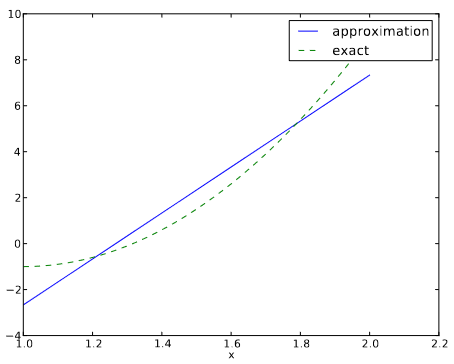
\includegraphics[width=0.7\linewidth]{img_3}
	\caption{Best approximation of a parabola by a straight line.}
	\label{fig:img_3}
\end{figure}
\section[Implementation of the least squares method]{Implementation of the least squares method}
\label{sec:sec_2_4}
\noindent The linear system can be computed either symbolically or numerically (a numer-
ical integration rule is needed in the latter case). Here is a function for symbolic
computation of the linear system, where f (x) is given as a sympy expression f
involving the symbol x, psi is a list of expressions for $\left\{\psi_{i}\right\}_{i \in \mathcal{I}_{s}}$, and Omega is a 2-tuple/list holding the limits of the domain $\Omega$ :

\begin{lstlisting}[numbers=none]
	import sympy as sp
	def least_squares(f, psi, Omega):
		N = len(psi) - 1
		A = sp.zeros((N+1, N+1))
		b = sp.zeros((N+1, 1))
		x = sp.Symbol('x')
		for i in range(N+1):
			for j in range(i, N+1):
				A[i,j] = sp.integrate(psi[i]*psi[j],
									(x, Omega[0], Omega[1]))
				A[j,i] = A[i,j]
			b[i,0] = sp.integrate(psi[i]*f, (x, Omega[0], Omega[1]))
		c = A.LUsolve(b)
		u = 0
		for i in range(len(psi)):
			u += c[i,0]*psi[i]
		return u, c
\end{lstlisting}
Observe that we exploit the symmetry of the coefficient matrix: only the
upper triangular part is computed. Symbolic integration in sympy is often
time consuming, and (roughly) halving the work has noticeable effect on the
waiting time for the function to finish execution.

Comparing the given f (x) and the approximate u(x) visually is done by
the following function, which with the aid of sympy's lambdify tool converts a
sympy expression to a Python function for numerical computations:
\begin{lstlisting}[numbers=none]
	def comparison_plot(f, u, Omega, filename='tmp.pdf'):
		x = sp.Symbol('x')
		f = sp.lambdify([x], f, modules="numpy")
		u = sp.lambdify([x], u, modules="numpy")
		resolution = 401 # no of points in plot
		xcoor = linspace(Omega[0], Omega[1], resolution)
		exact = f(xcoor)
		approx = u(xcoor)
		plot(xcoor, approx)
		hold('on')
		plot(xcoor, exact)
		legend(['approximation', 'exact'])
		savefig(filename)
\end{lstlisting}
The modules='numpy' argument to lambdify is important if there are mathe-
matical functions, such as sin or exp in the symbolic expressions in f or u, and
these mathematical functions are to be used with vector arguments, like xcoor
above.

Both the least\textunderscore squares and comparison\textunderscore plot are found and coded in the
file \href{http://tinyurl.com/jvzzcfn/fem/approx1D.py}{approx1D.py.} The forthcoming examples on their use appear in ex\textunderscore approx1D.py.
\section[Perfect approximation]{Perfect approximation}
\label{sec:sec_2_5}
Let us use the code above to recompute the problem from Section \hyperref[sec:sec_2_3]{2.3} where we want to approximate a parabola. What happens if we add an element $x^{2}$ to the basis and test what the best approximation is if V is the space of all parabolic
functions? The answer is quickly found by running
\begin{lstlisting}[numbers=none]
>>> from approx1D import *
>>> x = sp.Symbol('x')
>>> f = 10*(x-1)**2-1
>>> u, c = least_squares(f=f, psi=[1, x, x**2], Omega=[1, 2])
>>> print u
10*x**2 - 20*x + 9
>>> print sp.expand(f)
10*x**2 - 20*x + 9
\end{lstlisting}
Now, what if we use $\psi_{i}(x)=x^{i}$ for $i=0,1, \ldots, N=40$ ? The output from least\textunderscore squares gives $c_{i}=0$ for $i>2$, which means that the method finds the perfect approximation.

In fact, we have a general result that if $f \in V$, the least squares and projection/Galerkin methods compute the exact solution $u=f$. The proof is straightforward: if $f \in V, f$ can be expanded in terms of the basis functions, $f=\sum_{j \in \mathcal{I}_{s}} d_{j} \psi_{j}$, for some coefficients $\left\{d_{i}\right\}_{i \in \mathcal{I}_{s}}$, and the right-hand side then has entries
$$
b_{i}=\left(f, \psi_{i}\right)=\sum_{j \in \mathcal{I}_{s}} d_{j}\left(\psi_{j}, \psi_{i}\right)=\sum_{j \in \mathcal{I}_{s}} d_{j} A_{i, j}.
$$
The linear system $\sum_{j} A_{i, j} c_{j}=b_{i}, i \in \mathcal{I}_{s}$, is then
$$
\sum_{j \in \mathcal{I}_{s}} c_{j} A_{i, j}=\sum_{j \in \mathcal{I}_{s}} d_{j} A_{i, j}, \quad i \in \mathcal{I}_{s},
$$
which implies that $c_{i}=d_{i}$ for $i \in \mathcal{I}_{s}$.
\section[Ill-conditioning]{Ill-conditioning}
\label{sec:sec_2_6}
The computational example in Section \hyperref[sec:sec_2_5]{2.5} applies the least\textunderscore squares function which invokes symbolic methods to calculate and solve the linear system. The correct solution $c_{0}=9, c_{1}=-20, c_{2}=10, c_{i}=0$ for $i \geq 3$ is perfectly recovered.

Suppose we convert the matrix and right-hand side to floating-point arrays and then solve the system using finite-precision arithmetics, which is what one will (almost) always do in real life. This time we get astonishing results! Up to about $N=7$ we get a solution that is reasonably close to the exact one. Increasing $N$ shows that seriously wrong coefficients are computed. Below is a table showing the solution of the linear system arising from approximating a parabola by functions on the form $u(x)=c_{0}+c_{1} x+c_{2} x^{2}+\cdots+c_{10} x^{10}$. Analytically, we know that $c_{j}=0$ for $j>2$, but numerically we may get $c_{j} \neq 0$ for $j>2$.

\begin{tabular}{rrrr}
	\hline exact & sympy & numpy32 & numpy64 \\
	\hline 9 & $9.62$ & $5.57$ & $8.98$ \\
	$-20$ & $-23.39$ & $-7.65$ & $-19.93$ \\
	10 & $17.74$ & $-4.50$ & $9.96$ \\
	0 & $-9.19$ & $4.13$ & $-0.26$ \\
	0 & $5.25$ & $2.99$ & $0.72$ \\
	0 & $0.18$ & $-1.21$ & $-0.93$ \\
	0 & $-2.48$ & $-0.41$ & $0.73$ \\
	0 & $1.81$ & $-0.013$ & $-0.36$ \\
	0 & $-0.66$ & $0.08$ & $0.11$ \\
	0 & $0.12$ & $0.04$ & $-0.02$ \\
	0 & $-0.001$ & $-0.02$ & $0.002$ \\
	\hline
\end{tabular}
\bigbreak
\noindent The exact value of $c_{j}, j=0,1, \ldots, 10$, appears in the first column while the other columns correspond to results obtained by three different methods:
\begin{itemize}
	\item Column 2: The matrix and vector are converted to the data structure sympy .mpmath.fp.matrix and the sympy.mpmath.fp.lu\textunderscore solve function is used to solve the system.
	\item Column 3: The matrix and vector are converted to numpy arrays with data type numpy.float32 (single precision floating-point number) and solved by the numpy.linalg.solve function.
	\item Column 4: As column 3, but the data type is numpy.float64 (double precision floating-point number).
\end{itemize}

\noindent We see from the numbers in the table that double precision performs much better than single precision. Nevertheless, when plotting all these solutions the curves cannot be visually distinguished (!). This means that the approximations look perfect, despite the partially very wrong values of the coefficients.

Increasing $N$ to 12 makes the numerical solver in numpy abort with the message: "matrix is numerically singular". A matrix has to be non-singular to be invertible, which is a requirement when solving a linear system. Already when the matrix is close to singular, it is \textit{ill-conditioned}, which here implies that the numerical solution algorithms are sensitive to round-off errors and may produce (very) inaccurate results.

The reason why the coefficient matrix is nearly singular and ill-conditioned is that our basis functions $\psi_{i}(x)=x^{i}$ are nearly linearly dependent for large $i$. That is, $x^{i}$ and $x^{i+1}$ are very close for $i$ not very small. This phenomenon is illustrated in Figure 4. There are 15 lines in this figure, but only half of them are visually distinguishable. Almost linearly dependent basis functions give rise to an ill-conditioned and almost singular matrix. This fact can be illustrated by computing the determinant, which is indeed very close to zero (recall that a zero determinant implies a singular and non-invertible matrix): $10^{-65}$ for $N=10$ and $10^{-92}$ for $N=12$. Already for $N=28$ the numerical determinant computation returns a plain zero.
\begin{figure}[H]
	\centering
	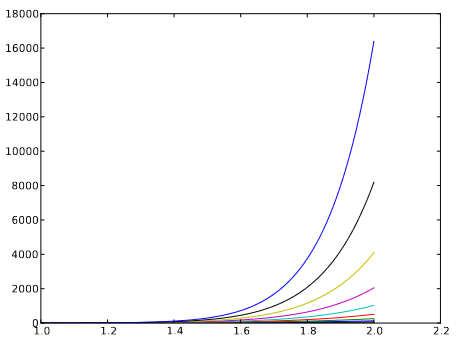
\includegraphics[width=0.7\linewidth]{img_4}
	\caption{The 15 first basis functions $x^{i}, i=0, \ldots, 14$.}
	\label{fig:img_4}
\end{figure}
On the other hand, the double precision numpy solver do run for $N=100$, resulting in answers that are not significantly worse than those in the table above, and large powers are associated with small coefficients (e.g., $c_{j}<10^{-2}$ for $10 \leq j \leq 20$ and $c<10^{-5}$ for $\left.j>20\right)$. Even for $N=100$ the approximation still lies on top of the exact curve in a plot (!).

The conclusion is that visual inspection of the quality of the approximation may not uncover fundamental numerical problems with the computations. However, numerical analysts have studied approximations and ill-conditioning for decades, and it is well known that the basis \{1, $x^{2}$, $x^{3}$, \ldots, \} is a bad basis. The best basis from a matrix conditioning point of view is to have orthogonal functions such that $\left(\psi_{i}, \psi_{j}\right)=0$ for $i \neq j$. There are many known sets of orthogonal polynomials and other functions. The functions used in the finite element methods are almost orthogonal, and this property helps to avoid problems with solving matrix systems. Almost orthogonal is helpful, but not enough when it comes to partial differential equations, and ill-conditioning of the coefficient matrix is a theme when solving large-scale matrix systems arising from finite element discretizations.
\bigbreak
\section[Fourier series]{Fourier series}
\label{sec:sec_2_7}
\noindent A set of sine functions is widely used for approximating functions (the sines are
also orthogonal as explained more in Section \hyperref[sec:sec_2_6]{2.6}). Let us take

$$
V=\operatorname{span}\{\sin \pi x, \sin 2 \pi x, \ldots, \sin (N+1) \pi x\}.
$$
That is,
$$
\psi_{i}(x)=\sin ((i+1) \pi x), \quad i \in \mathcal{I}_{s} .
$$
An approximation to the $f(x)$ function from Section \hyperref[sec:sec_2_3]{2.3} can then be computed by the least\textunderscore squares function from Section \hyperref[sec:sec_2_4]{2.4}:
\begin{lstlisting}[numbers=none]
N = 3
from sympy import sin, pi
x = sp.Symbol('x')
psi = [sin(pi*(i+1)*x) for i in range(N+1)]
f = 10*(x-1)**2 - 1
Omega = [0, 1]
u, c = least_squares(f, psi, Omega)
comparison_plot(f, u, Omega)
\end{lstlisting}
Figure \hyperref[fig:img_5]{5} (left) shows the oscillatory approximation of $\sum_{j-0}^{N} c_{j} \sin ((j+1) \pi x)$ when $N=3$. Changing $N$ to 11 improves the approximation considerably, see Figure \hyperref[fig:img_5]{5} (right).
\begin{figure}[H]
	\centering
	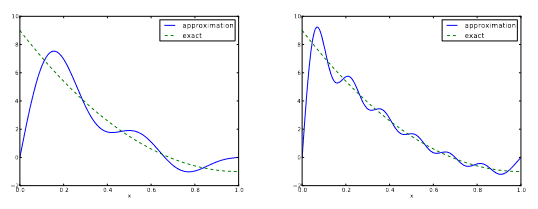
\includegraphics[width=0.7\linewidth]{img_5}
	\caption{Best approximation of a parabola by a sum of 3 (left) and 11 (right) sine functions.}
	\label{fig:img_5}
\end{figure}

There is an error $f(0)-u(0)=9$ at $x=0$ in Figure \hyperref[fig:img_5]{5} regardless of how large $N$ is, because all $\psi_{i}(0)=0$ and hence $u(0)=0$. We may help the approximation to be correct at $x=0$ by seeking
\begin{equation}\label{eqa39}
	u(x)=f(0)+\sum_{j \in \mathcal{I}_{s}} c_{j} \psi_{j}(x).
\end{equation}
However, this adjustment introduces a new problem at $x=1$ since we now get an error $f(1)-u(1)=f(1)-0=-1$ at this point. A more clever adjustment is to replace the $f(0)$ term by a term that is $f(0)$ at $x=0$ and $f(1)$ at $x=1$. A simple linear combination $f(0)(1-x)+x f(1)$ does the job:
\begin{equation}\label{eqa40}
	u(x)=f(0)(1-x)+x f(1)+\sum_{j \in \mathcal{I}_{s}} c_{j} \psi_{j}(x).
\end{equation}
\noindent This adjustment of $u$ alters the linear system slightly as we get an extra term $-\left(f(0)(1-x)+x f(1), \psi_{i}\right)$ on the right-hand side. Figure \hyperref[fig:img_6]{6} shows the result of this technique for ensuring right boundary values: even 3 sines can now adjust the $f(0)(1-x)+x f(1)$ term such that $u$ approximates the parabola really well, at least visually.
\begin{figure}[H]
	\centering
	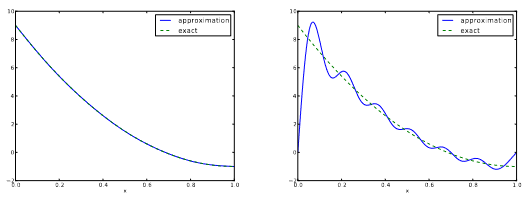
\includegraphics[width=0.7\linewidth]{img_6}
	\caption{Best approximation of a parabola by a sum of 3 (left) and 11 (right)
		sine functions with a boundary term.}
	\label{fig:img_6}
\end{figure}
\section[Orthogonal basis functions]{Orthogonal basis functions}
\label{sec:sec_2_8}
The choice of sine functions $\psi_{i}(x)=\sin ((i+1) \pi x)$ has a great computational advantage: on $\Omega=[0,1]$ these basis functions are \textit{orthogonal}, implying that $A_{i, j}=0$ if $i \neq j$. This result is realized by trying
\begin{lstlisting}[numbers=none]
integrate(sin(j*pi*x)*sin(k*pi*x), x, 0, 1)
\end{lstlisting}
in \href{https://www.wolframalpha.com/}{WolframAlpha} (avoid i in the integrand as this symbol means the imaginary unit $\sqrt{-1})$. Also by asking WolframAlpha about $\int_{0}^{1} \sin ^{2}(j \pi x) \mathrm{d} x$, we find it to equal $1 / 2$. With a diagonal matrix we can easily solve for the coefficients by hand:
\begin{equation}\label{eqa41}
	c_{i}=2 \int_{0}^{1} f(x) \sin ((i+1) \pi x) \mathrm{d} x, \quad i \in \mathcal{I}_{s},
\end{equation}
which is nothing but the classical formula for the coefficients of the Fourier sine series of $f(x)$ on $[0,1]$. In fact, when $V$ contains the basic functions used in a Fourier series expansion, the approximation method derived in Section \hyperref[chap:chap_2]{2} results in the classical Fourier series for $f(x)$ (see Exercise \hyperref[sec:sec_10_8]{8} for details).

With orthogonal basis functions we can make the least\textunderscore squares function (much) more efficient since we know that the matrix is diagonal and only the diagonal elements need to be computed:
\begin{lstlisting}[numbers=none]
def least_squares_orth(f, psi, Omega):
	N = len(psi) - 1
	A = [0]*(N+1)
	b = [0]*(N+1)
	x = sp.Symbol('x')
	for i in range(N+1):
	A[i] = sp.integrate(psi[i]**2, (x, Omega[0], Omega[1]))
	b[i] = sp.integrate(psi[i]*f, (x, Omega[0], Omega[1]))
	c = [b[i]/A[i] for i in range(len(b))]
	u = 0
	for i in range(len(psi)):
	u += c[i]*psi[i]
	return u, c
\end{lstlisting}
This function is found in the file approx1D.py.
\section[Numerical computations]{Numerical computations}
\label{sec:sec_2_9}
\noindent Sometimes the basis functions $\psi_{i}$ and/or the function $f$ have a nature that makes symbolic integration CPU-time consuming or impossible. Even though we implemented a fallback on numerical integration of $\int f \varphi_{i} d x$ considerable time might be required by sympy in the attempt to integrate symbolically. Therefore, it will be handy to have function for fast \textit{numerical} integration and \textit{numerical} solution of the linear system. Below is such a method. It requires Python functions $\mathrm{f}(\mathrm{x})$ and psi $(\mathrm{x}, i)$ for $f(x)$ and $\psi_{i}(x)$ as input. The output is a mesh function with values $u$ on the mesh with points in the array $x$. Three numerical integration methods are offered: scipy. integrate. quad (precision set to $10^{-8}$ ), sympy -mpmath . quad (high precision), and a Trapezoidal rule based on the points in $x$.
\begin{lstlisting}[numbers=none]
def least_squares_numerical(f, psi, N, x,
							integration_method='scipy',
							orthogonal_basis=False):
	import scipy.integrate
	A = np.zeros((N+1, N+1))
	b = np.zeros(N+1)
	Omega = [x[0], x[-1]]
	dx = x[1] - x[0]
	
	for i in range(N+1):
		j_limit = i+1 if orthogonal_basis else N+1
		for j in range(i, j_limit):
			print '(%d,%d)' % (i, j)
			if integration_method == 'scipy':
				A_ij = scipy.integrate.quad(
					lambda x: psi(x,i)*psi(x,j),
					Omega[0], Omega[1], epsabs=1E-9, epsrel=1E-9)[0]
			elif integration_method == 'sympy':
				A_ij = sp.mpmath.quad(
					lambda x: psi(x,i)*psi(x,j),
					[Omega[0], Omega[1]])
			else:
				values = psi(x,i)*psi(x,j)
				A_ij = trapezoidal(values, dx)
			A[i,j] = A[j,i] = A_ij
			
		if integration_method == 'scipy':
			b_i = scipy.integrate.quad(			
				lambda x: f(x)*psi(x,i), Omega[0], Omega[1],
				epsabs=1E-9, epsrel=1E-9)[0]
		elif integration_method == 'sympy':
			b_i = sp.mpmath.quad(
				lambda x: f(x)*psi(x,i), [Omega[0], Omega[1]])
		else:
			values = f(x)*psi(x,i)
			b_i = trapezoidal(values, dx)
		b[i] = b_i
		
	c = b/np.diag(A) if orthogonal_basis else np.linalg.solve(A, b)
	u = sum(c[i]*psi(x, i) for i in range(N+1))
	return u, c
	
def trapezoidal(values, dx):
	"""Integrate values by the Trapezoidal rule (mesh size dx)."""
	return dx*(np.sum(values) - 0.5*values[0] - 0.5*values[-1])
\end{lstlisting}
Here is an example on calling the function:
\begin{lstlisting}[numbers=none]
from numpy import linspace, tanh, pi
def psi(x, i):
	return sin((i+1)*x)
x = linspace(0, 2*pi, 501)
N = 20
u, c = least_squares_numerical(lambda x: tanh(x-pi), psi, N, x,
								orthogonal_basis=True)
\end{lstlisting}
\section[The interpolation (or collocation) method]{The interpolation (or collocation) method}
\label{sec:sec_2_10}
The principle of minimizing the distance between $u$ and $f$ is an intuitive way of computing a best approximation $u \in V$ to $f$. However, there are other approaches as well. One is to demand that $u\left(x_{i}\right)=f\left(x_{i}\right)$ at some selected points $x_{i}, i \in \mathcal{I}_{s}$ :
\begin{equation}\label{eqa42}
	u\left(x_{i}\right)=\sum_{j \in \mathcal{I}_{s}} c_{j} \psi_{j}\left(x_{i}\right)=f\left(x_{i}\right), \quad i \in \mathcal{I}_{s}.
\end{equation}
This criterion also gives a linear system with $N+1$ unknown coefficients
$\left\{c_{i}\right\}_{i \in \mathcal{I}_{s}}$ :
\begin{equation}\label{eqa43}
	\sum_{j \in \mathcal{I}_{s}} A_{i, j} c_{j}=b_{i}, \quad i \in \mathcal{I}_{s},
\end{equation}
with
\begin{equation}\label{eqa44}
	A_{i, j} = \psi_{j}\left(x_{i}\right),
\end{equation}
\begin{equation}\label{eqa45}
	b_{i} = f\left(x_{i}\right).
\end{equation}
This time the coefficient matrix is not symmetric because $\psi_{j}\left(x_{i}\right) \neq \psi_{i}\left(x_{j}\right)$ in general. The method is often referred to as an \textit{interpolation method} since some point values of $f$ are given $\left(f\left(x_{i}\right)\right)$ and we fit a continuous function $u$ that goes through the $f\left(x_{i}\right)$ points. In this case the $x_{i}$ points are called \textit{interpolation points}. When the same approach is used to approximate differential equations, one usually applies the name \textit{collocation method} and $x_{i}$ are known as \textit{collocation points}.

Given $f$ as a sympy symbolic expression $\mathrm{f},\left\{\psi_{i}\right\}_{i \in \mathcal{I}_{s}}$ as a list psi, and a set of points $\left\{x_{i}\right\}_{i \in \mathcal{I}_{s}}$ as a list or array points, the following Python function sets up and solves the matrix system for the coefficients $\left\{c_{i}\right\}_{i \in \mathcal{I}_{s}}$ :
\begin{lstlisting}[numbers=none]
def interpolation(f, psi, points):
	N = len(psi) - 1
	A = sp.zeros((N+1, N+1))
	b = sp.zeros((N+1, 1))
	x = sp.Symbol('x')
	# Turn psi and f into Python functions
	psi = [sp.lambdify([x], psi[i]) for i in range(N+1)]
	f = sp.lambdify([x], f)
	for i in range(N+1):
		for j in range(N+1):
			A[i,j] = psi[j](points[i])
		b[i,0] = f(points[i])
	c = A.LUsolve(b)
	u = 0
	for i in range(len(psi)):
		u += c[i,0]*psi[i](x)
	return u	
\end{lstlisting}	
The interpolation function is a part of the approx1D module.

We found it convenient in the above function to turn the expressions f
and psi into ordinary Python functions of x, which can be called with float
values in the list points when building the matrix and the right-hand side.
The alternative is to use the subs method to substitute the x variable in an
expression by an element from the points list. The following session illustrates
both approaches in a simple setting:\\
\begin{lstlisting}[numbers=none]
>>> from sympy import *
>>> x = Symbol('x')
>>> e = x**2 # symbolic expression involving x
>>> p = 0.5 # a value of x
>>> v = e.subs(x, p) # evaluate e for x=p
>>> v
0.250000000000000
>>> type(v)
sympy.core.numbers.Float
>>> e = lambdify([x], e) # make Python function of e
>>> type(e)
>>> function
>>> v = e(p) # evaluate e(x) for x=p
>>> v
0.25
>>> type(v)
float	
\end{lstlisting}
A nice feature of the interpolation or collocation method is that it avoids computing integrals. However, one has to decide on the location of the $x_{i}$ points. A simple, yet common choice, is to distribute them uniformly throughout $\Omega$.
\bigbreak
\noindent \textbf{Example.} Let us illustrate the interpolation or collocation method by approximating our parabola $f(x)=10(x-1)^{2}-1$ by a linear function on $\Omega=[1,2]$, using two collocation points $x_{0}=1+1 / 3$ and $x_{1}=1+2 / 3$ :
\begin{lstlisting}[numbers=none]
f = 10*(x-1)**2 - 1
psi = [1, x]
Omega = [1, 2]
points = [1 + sp.Rational(1,3), 1 + sp.Rational(2,3)]
u = interpolation(f, psi, points)
comparison_plot(f, u, Omega)		
\end{lstlisting}
The resulting linear system becomes
$$
\left(\begin{array}{ll}
	1 & 4 / 3 \\
	1 & 5 / 3
\end{array}\right)\left(\begin{array}{l}
	c_{0} \\
	c_{1}
\end{array}\right)=\left(\begin{array}{l}
	1 / 9 \\
	31 / 9
\end{array}\right)
$$
with solution $c_{0}=-119 / 9$ and $c_{1}=10$. Figure \hyperref[fig:img_7]{7} (left) shows the resulting approximation $u=-119 / 9+10 x$. We can easily test other interpolation points, say $x_{0}=1$ and $x_{1}=2$. This changes the line quite significantly, see Figure \hyperref[fig:img_7]{7} (right).
\begin{figure}[H]
	\centering
	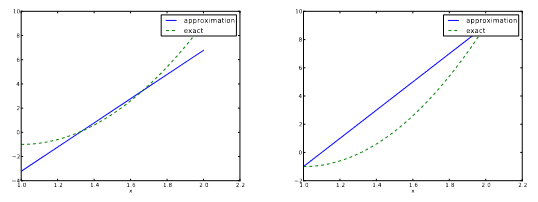
\includegraphics[width=0.7\linewidth]{img_7}
	\caption{Approximation of a parabola by linear functions computed by two
		interpolation points: 4/3 and 5/3 (left) versus 1 and 2 (right).}
	\label{fig:img_7}
\end{figure}
\section[Lagrange polynomials]{Lagrange polynomials}
\label{sec:sec_2_11}
\noindent In Section \hyperref[sec:sec_2_7]{2.7} we explain the advantage with having a diagonal matrix: formulas for the coefficients $\left\{c_{i}\right\}_{i \in \mathcal{I}_{s}}$ can then be derived by hand. For an interpolation/collocation method a diagonal matrix implies that $\psi_{j}\left(x_{i}\right)=0$ if $i \neq j$. One set of basis functions $\psi_{i}(x)$ with this property is the Lagrange interpolating polynomials, or just \textit{Lagrange polynomials}. (Although the functions are named after Lagrange, they were first discovered by Waring in 1779 , rediscovered by
Euler in 1783 , and published by Lagrange in 1795.) The Lagrange polynomials have the form
\begin{equation}\label{eqa46}
	\psi_{i}(x)=\prod_{j=0, j \neq i}^{N} \frac{x-x_{j}}{x_{i}-x_{j}}=\frac{x-x_{0}}{x_{i}-x_{0}} \cdots \frac{x-x_{i-1}}{x_{i}-x_{i-1}} \frac{x-x_{i+1}}{x_{i}-x_{i+1}} \cdots \frac{x-x_{N}}{x_{i}-x_{N}},
\end{equation}
for $i \in \mathcal{I}_{s}$. We see from (\hyperref[eqa46]{46}) that all the $\psi_{i}$ functions are polynomials of degree $N$ which have the property
\begin{equation}\label{eqa47}
	\psi_{i}\left(x_{s}\right)=\delta_{i s}, \quad \delta_{i s}= \begin{cases}1, & i=s, \\ 0, & i \neq s,\end{cases}
\end{equation}
when $x_{s}$ is an interpolation/collocation point. Here we have used the \textit{Kronecker delta} symbol $\delta_{i s}$. This property implies that $A_{i, j}=0$ for $i \neq j$ and $A_{i, j}=1$ when $i=j$. The solution of the linear system is them simply
\begin{equation}\label{eqa48}
	c_{i}=f\left(x_{i}\right), \quad i \in \mathcal{I}_{s},
\end{equation}
and
\begin{equation}\label{eqa49}
	u(x)=\sum_{j \in \mathcal{I}_{s}} f\left(x_{i}\right) \psi_{i}(x).
\end{equation}
The following function computes the Lagrange interpolating polynomial $\psi_{i}(x)$, given the interpolation points $x_{0}, \ldots, x_{N}$ in the list or array points:
\begin{lstlisting}[numbers=none]
def Lagrange_polynomial(x, i, points):
	p = 1
	for k in range(len(points)):
		if k != i:
			p *= (x - points[k])/(points[i] - points[k])
	return p
\end{lstlisting}
The next function computes a complete basis using equidistant points throughout
$\Omega$:
\begin{lstlisting}[numbers=none]
def Lagrange_polynomials_01(x, N):
	if isinstance(x, sp.Symbol):
		h = sp.Rational(1, N-1)
	else:
		h = 1.0/(N-1)
	points = [i*h for i in range(N)]
	psi = [Lagrange_polynomial(x, i, points) for i in range(N)]
	return psi, points	
\end{lstlisting}
When $x$ is an sp. Symbol object, we let the spacing between the interpolation points, $\mathrm{h}$, be a sympy rational number for nice end results in the formulas for $\psi_{i}$. The other case, when $\mathrm{x}$ is a plain Python $\mathrm{float}$, signifies numerical computing, and then we let $\mathrm{h}$ be a floating-point number. Observe that the Lagrange\textunderscore polynomial function works equally well in the symbolic and numerical case - just think of x being an sp.Symbol object or a Python float. A little
interactive session illustrates the difference between symbolic and numerical
computing of the basis functions and points:
\begin{lstlisting}[numbers=none]
>>> import sympy as sp
>>> x = sp.Symbol('x')
>>> psi, points = Lagrange_polynomials_01(x, N=3)
>>> points
[0, 1/2, 1]
>>> psi
[(1 - x)*(1 - 2*x), 2*x*(2 - 2*x), -x*(1 - 2*x)]
>>> x = 0.5 # numerical computing
>>> psi, points = Lagrange_polynomials_01(x, N=3)
>>> points
[0.0, 0.5, 1.0]
>>> psi
[-0.0, 1.0, 0.0]	
\end{lstlisting}
The Lagrange polynomials are very much used in finite element methods because
of their property (\hyperref[eqa47]{47}).

\noindent \textbf{Approximation of a polynomial.} The Galerkin or least squares method lead
to an exact approximation if f lies in the space spanned by the basis functions. It
could be interest to see how the interpolation method with Lagrange polynomials
as basis is able to approximate a polynomial, e.g., a parabola. Running
\begin{lstlisting}[numbers=none]
for N in 2, 4, 5, 6, 8, 10, 12:
	f = x**2
	psi, points = Lagrange_polynomials_01(x, N)
	u = interpolation(f, psi, points)	
\end{lstlisting}
shows the result that up to $\mathrm{N}=4$ we achieve an exact approximation, and then round-off errors start to grow, such that $\mathrm{N}=15$ leads to a 15 -degree polynomial for $u$ where the coefficients in front of $x^{r}$ for $r>2$ are of size $10^{-5}$ and smaller.
Successful example. Trying out the Lagrange polynomial basis for approximating $f(x)=\sin 2 \pi x$ on $\Omega=[0,1]$ with the least squares and the interpolation techniques can be done by
\begin{lstlisting}[numbers=none]
x = sp.Symbol('x')
f = sp.sin(2*sp.pi*x)
psi, points = Lagrange_polynomials_01(x, N)
Omega=[0, 1]
u = least_squares(f, psi, Omega)
comparison_plot(f, u, Omega)
u = interpolation(f, psi, points)
comparison_plot(f, u, Omega)	
\end{lstlisting}
Figure \hyperref[fig:img_8]{8} shows the results. There is little difference between the least squares and
the interpolation technique. Increasing \textit{N} gives visually better approximations.
\begin{figure}[H]
	\centering
	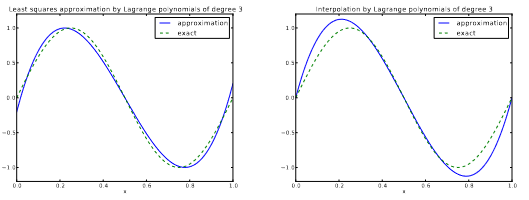
\includegraphics[width=0.7\linewidth]{img_8}
	\caption{Approximation via least squares (left) and interpolation (right) of a
		sine function by Lagrange interpolating polynomials of degree 3.}
	\label{fig:img_8}
\end{figure}	

\noindent \textbf{Less successful example.} The next example concerns interpolating $f(x)=$ $|1-2 x|$ on $\Omega=[0,1]$ using Lagrange polynomials. Figure \hyperref[fig:img_9]{9} shows a peculiar effect: the approximation starts to oscillate more and more as $N$ grows. This numerical artifact is not surprising when looking at the individual Lagrange polynomials. Figure \hyperref[fig:img_10]{10} shows two such polynomials, $\psi_{2}(x)$ and $\psi_{7}(x)$, both of degree 11 and computed from uniformly spaced points $x_{x_{i}}=i / 11, i=0, \ldots, 11$, marked with circles. We clearly see the property of Lagrange polynomials: $\psi_{2}\left(x_{i}\right)=0$ and $\psi_{7}\left(x_{i}\right)=0$ for all $i$, except $\psi_{2}\left(x_{2}\right)=1$ and $\psi_{7}\left(x_{7}\right)=1$. The most striking feature, however, is the significant oscillation near the boundary. The reason is easy to understand: since we force the functions to zero at so many points, a polynomial of high degree is forced to oscillate between the points. The points, a polynomial of high degree is forced to oscillate between the points. The phenomenon is named Runge's phenomenon and you can read a more detailed explanation on \href{https://en.wikipedia.org/wiki/Runge%27s_phenomenon}{Wikipedia}.
\bigbreak
\noindent \textbf{Remedy for strong oscillations.} The oscillations can be reduced by a more clever choice of interpolation points, called the \textit{Chebyshev nodes}:
\begin{equation}\label{eqa50}
	x_{i}=\frac{1}{2}(a+b)+\frac{1}{2}(b-a) \cos \left(\frac{2 i+1}{2(N+1)} p i\right), \quad i=0 \ldots, N,
\end{equation}
on the interval $\Omega=[a, b]$. Here is a flexible version of the Lagrange\textunderscore polynomials\textunderscore 01 function above, valid for any interval $\Omega=[a, b]$ and with the possibility to generate both uniformly distributed points and Chebyshev nodes:
\begin{lstlisting}[numbers=none]
def Lagrange_polynomials(x, N, Omega, point_distribution='uniform'):
	if point_distribution == 'uniform':
		if isinstance(x, sp.Symbol):
			h = sp.Rational(Omega[1] - Omega[0], N)
		else:
			h = (Omega[1] - Omega[0])/float(N)
		points = [Omega[0] + i*h for i in range(N+1)]
	elif point_distribution == 'Chebyshev':
		points = Chebyshev_nodes(Omega[0], Omega[1], N)
	psi = [Lagrange_polynomial(x, i, points) for i in range(N+1)]
	return psi, points
def Chebyshev_nodes(a, b, N):
	from math import cos, pi
	return [0.5*(a+b) + 0.5*(b-a)*cos(float(2*i+1)/(2*N+1))*pi) \
			for i in range(N+1)]
\end{lstlisting}
All the functions computing Lagrange polynomials listed above are found in the module file Lagrange.py. Figure 11 shows the improvement of using Chebyshev nodes (compared with Figure \hyperref[fig:img_9]{9}). The reason is that the corresponding Lagrange polynomials have much smaller oscillations as seen in Figure \hyperref[fig:img_12]{12} (compare with Figure \hyperref[fig:img_10]{10}).

Another cure for undesired oscillation of higher-degree interpolating polynomials is to use lower-degree Lagrange polynomials on many small patches of the domain, which is the idea pursued in the finite element method. For instance, linear Lagrange polynomials on $[0,1 / 2]$ and $[1 / 2,1]$ would yield a perfect approximation to $f(x)=|1-2 x|$ on $\Omega=[0,1]$ since $f$ is piecewise linear.
\begin{figure}[H]
	\centering
	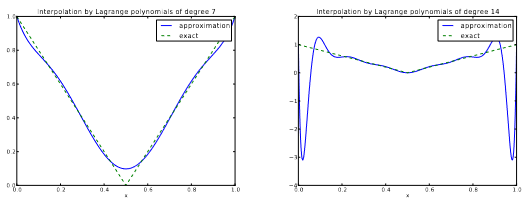
\includegraphics[width=0.7\linewidth]{img_9}
	\caption{Interpolation of an absolute value function by Lagrange polynomials and uniformly distributed interpolation points: degree 7 (left) and 14 (right).}
	\label{fig:img_9}
\end{figure}
How does the least squares or projection methods work with Lagrange polynomials? Unfortunately, sympy has problems integrating the $f(x)=|1-2 x|$ function times a polynomial. Other choices of $f(x)$ can also make the symbolic integration fail. Therefore, we should extend the least\textunderscore squares function such that it falls back on numerical integration if the symbolic integration is unsuccessful. In the latter case, the returned value from sympy's integrate function is an object of type Integral. We can test on this type and utilize the mpmath module in sympy to perform numerical integration of high precision. Here is the code:
\begin{lstlisting}[numbers=none]
def least_squares(f, psi, Omega):
	N = len(psi) - 1
	A = sp.zeros((N+1, N+1))
	b = sp.zeros((N+1, 1))
	x = sp.Symbol('x')
	for i in range(N+1):
		for j in range(i, N+1):
			integrand = psi[i]*psi[j]
			I = sp.integrate(integrand, (x, Omega[0], Omega[1]))	
\end{lstlisting}
\begin{figure}[H]
	\centering
	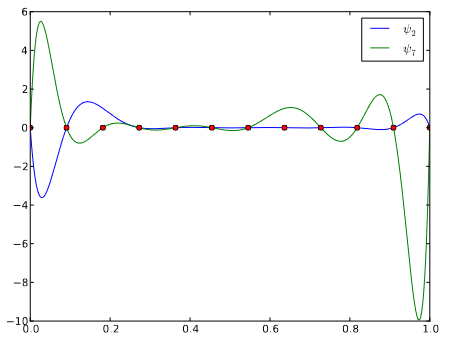
\includegraphics[width=0.7\linewidth]{img_10}
	\caption{Illustration of the oscillatory behavior of two Lagrange polynomials
		based on 12 uniformly spaced points (marked by circles).}
	\label{fig:img_10}
\end{figure}
\begin{figure}[H]
	\centering
	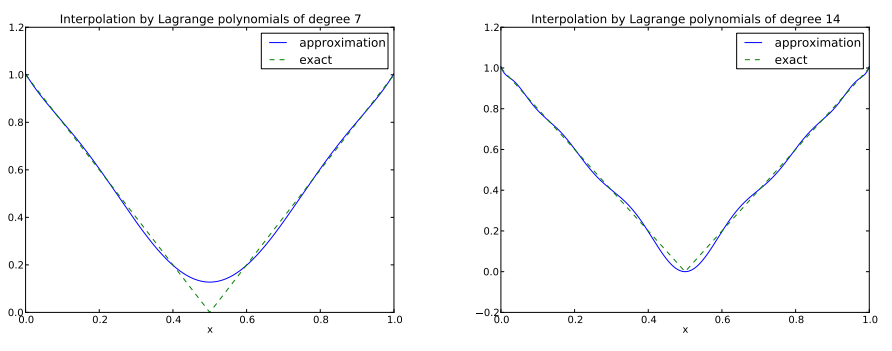
\includegraphics[width=0.7\linewidth]{img_11}
	\caption{ Interpolation of an absolute value function by Lagrange polynomials
		and Chebyshev nodes as interpolation points: degree 7 (left) and 14 (right).}
	\label{fig:img_11}
\end{figure}
\begin{lstlisting}[numbers=none]
			if isinstance(I, sp.Integral):
				# Could not integrate symbolically, fallback
				# on numerical integration with mpmath.quad
				integrand = sp.lambdify([x], integrand)
				I = sp.mpmath.quad(integrand, [Omega[0], Omega[1]])
			A[i,j] = A[j,i] = I
		integrand = psi[i]*f
		I = sp.integrate(integrand, (x, Omega[0], Omega[1]))
		if isinstance(I, sp.Integral):
			integrand = sp.lambdify([x], integrand)
\end{lstlisting}
\begin{figure}[H]
	\centering
	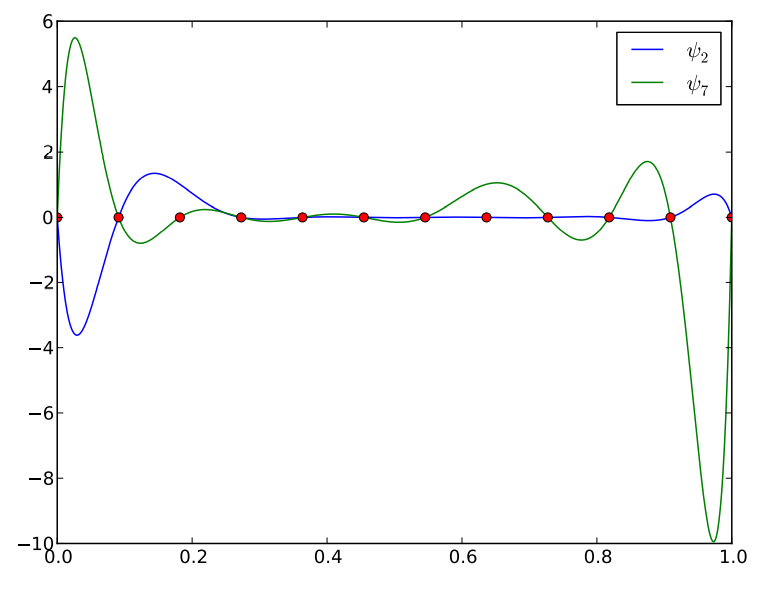
\includegraphics[width=0.7\linewidth]{img_12}
	\caption{Illustration of the less oscillatory behavior of two Lagrange polynomials based on 12 Chebyshev points (marked by circles).}
	\label{fig:img_12}
\end{figure}
\begin{lstlisting}[numbers=none]
			I = sp.mpmath.quad(integrand, [Omega[0], Omega[1]])
		b[i,0] = I
	c = A.LUsolve(b)
	u = 0
	for i in range(len(psi)):
		u += c[i,0]*psi[i]
	return u
\end{lstlisting}

\chapter{Finite element basis functions}
\label{chap:chap_3}
\noindent The specific basis functions exemplified in Section \hyperref[chap:chap_2]{2} are in general nonzero on the entire domain $\Omega$, see Figure \hyperref[fig:img_13]{13} for an example where we plot $\psi_{0}(x)=\sin \frac{1}{2} \pi x$ and $\psi_{1}(x)=\sin 2 \pi x$ together with a possible sum $u(x)=4 \psi_{0}(x)-\frac{1}{2} \psi_{1}(x)$. We shall now turn the attention to basis functions that have compact support, meaning that they are nonzero on only a small portion of $\Omega$. Moreover, we shall restrict the functions to be \textit{piecewise polynomials}. This means that the domain is split into subdomains and the function is a polynomial on one or more subdomains, see Figure \hyperref[fig:img_14]{14} for a sketch involving locally defined hat functions that make $u=\sum_{j} c_{j} \psi_{j}$ piecewise linear. At the boundaries between subdomains one normally forces continuity of the function only so that when connecting two polynomials from two subdomains, the derivative becomes discontinuous. These type of basis functions are fundamental in the finite element method.
\begin{figure}[H]
	\centering
	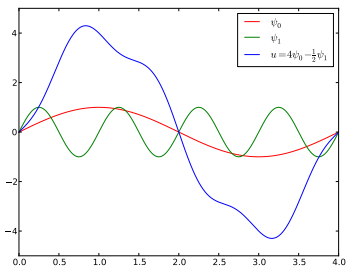
\includegraphics[width=0.7\linewidth]{img_13}
	\caption{A function resulting from adding two sine basis functions.}
	\label{fig:img_13}
\end{figure}
We first introduce the concepts of elements and nodes in a simplistic fashion
as often met in the literature. Later, we shall generalize the concept of an
element, which is a necessary step to treat a wider class of approximations within
the family of finite element methods. The generalization is also compatible with
the concepts used in the \href{https://fenicsproject.org/}{FEniCS} finite element software
\section[Elements and nodes]{Elements and nodes}
\label{sec:sec_3_1}
Let us divide the interval $\Omega$ on which $f$ and $u$ are defined into non-overlapping subintervals $\Omega^{(e)}, e=0, \ldots, N_{e}$ :
\begin{equation}\label{eqa51}
	\Omega=\Omega^{(0)} \cup \cdots \cup \Omega^{\left(N_{c}\right)}.
\end{equation}
We shall for now refer to $\Omega^{(e)}$ as an element, having number $e$. On each element we introduce a set of points called nodes. For now we assume that the nodes are uniformly spaced throughout the element and that the boundary points of the elements are also nodes. The nodes are given numbers both within an element and in the global domain. These are referred to as \textit{local} and \textit{global} node numbers, respectively. Figure \hyperref[fig:img_15]{15} shows element boundaries with small vertical lines, nodes as small disks, element numbers in circles, and global node numbers under the nodes.

Nodes and elements uniquely define a \textit{finite element mesh}, which is our discrete representation of the domain in the computations. A common special
\begin{figure}[H]
	\centering
	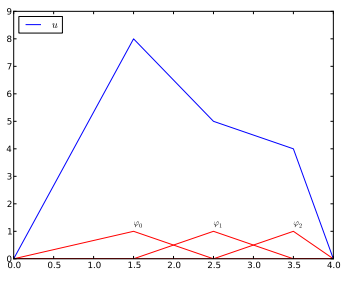
\includegraphics[width=0.7\linewidth]{img_14}
	\caption{A function resulting from adding three local piecewise linear (hat)
		functions.}
	\label{fig:img_14}
\end{figure}
\begin{figure}[H]
	\centering
	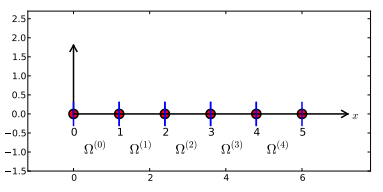
\includegraphics[width=0.7\linewidth]{img_15}
	\caption{Finite element mesh with 5 elements and 6 nodes.}
	\label{fig:img_15}
\end{figure}

\noindent case is that of a \textit{uniformly partitioned mesh} where each element has the same
length and the distance between nodes is constant.

\noindent \textbf{Example.} $\quad$ On $\Omega=[0,1]$ we may introduce two elements, $\Omega^{(0)}=[0,0.4]$ and $\Omega^{(1)}=[0.4,1]$. Furthermore, let us introduce three nodes per element, equally spaced within each element. Figure \hyperref[fig:img_16]{16} shows the mesh. The three nodes in element number 0 are $x_{0}=0, x_{1}=0.2$, and $x_{2}=0.4$. The local and global node numbers are here equal. In element number 1 , we have the local nodes $x_{0}=0.4$, $x_{1}=0.7$, and $x_{2}=1$ and the corresponding global nodes $x_{2}=0.4, x_{3}=0.7$, and $x_{4}=1$. Note that the global node $x_{2}=0.4$ is shared by the two elements.
\begin{figure}[H]
	\centering
	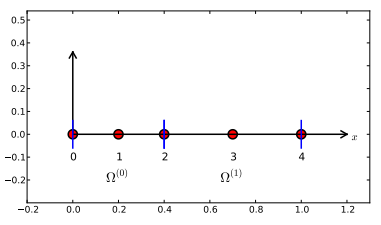
\includegraphics[width=0.7\linewidth]{img_16}
	\caption{Finite element mesh with 2 elements and 5 nodes.}
	\label{fig:img_16}
\end{figure}

For the purpose of implementation, we introduce two lists or arrays: nodes
for storing the coordinates of the nodes, with the global node numbers as indices,
and elements for holding the global node numbers in each element, with the
local node numbers as indices. The nodes and elements lists for the sample
mesh above take the form
\begin{lstlisting}[numbers=none]
nodes = [0, 0.2, 0.4, 0.7, 1]
elements = [[0, 1, 2], [2, 3, 4]]	
\end{lstlisting}
Looking up the coordinate of local node number 2 in element 1 is here done by
nodes[elements[1][2]] (recall that nodes and elements start their numbering
at 0).

The numbering of elements and nodes does not need to be regular. Figure \hyperref[fig:img_17]{17}
shows and example corresponding to
\begin{lstlisting}[numbers=none]
nodes = [1.5, 5.5, 4.2, 0.3, 2.2, 3.1]
elements = [[2, 1], [4, 5], [0, 4], [3, 0], [5, 2]]	
\end{lstlisting}
\section[The basis functions]{The basis functions}
\label{sec:sec_3_2}
\noindent \textbf{Construction principles}. Finite element basis functions are in this text recognized by the notation $\varphi_{i}(x)$, where the index now in the beginning corresponds to a global node number. In the current approximation problem we shall simply take $\psi_{i}=\varphi_{i}$.

Let $i$ be the global node number corresponding to local node $r$ in element number $e$. The finite element basis functions $\varphi_{i}$ are now defined as follows.
\begin{figure}[H]
	\centering
	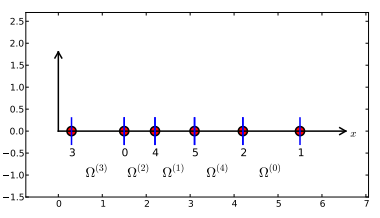
\includegraphics[width=0.7\linewidth]{img_17}
	\caption{Example on irregular numbering of elements and nodes.}
	\label{fig:img_17}
\end{figure}

\begin{itemize}
	\item If local node number $r$ is not on the boundary of the element, take $\varphi_{i}(x)$ to be the Lagrange polynomial that is 1 at the local node number $r$ and zero at all other nodes in the element. On all other elements, $\varphi_{i}=0$.
	\item If local node number $r$ is on the boundary of the element, let $\varphi_{i}$ be made up of the Lagrange polynomial over element $e$ that is 1 at node $i$, combined with the Lagrange polynomial over element $e+1$ that is also 1 at node $i$. On all other elements, $\varphi_{i}=0$.
\end{itemize}
A visual impression of three such basis functions are given in Figure $18 .$
\bigbreak
\noindent \textbf{Properties of} $\varphi_{i}$. The construction of basis functions according to the principles above lead to two important properties of $\varphi_{i}(x)$. First,
\begin{equation}\label{eqa52}
	\varphi_{i}\left(x_{j}\right)=\delta_{i j}, \quad \delta_{i j}= \begin{cases}1, & i=j, \\ 0, & i \neq j,\end{cases}
\end{equation}
when $x_{j}$ is a node in the mesh with global node number $j$. The result $\varphi_{i}\left(x_{j}\right)=\delta_{i j}$ arises because the Lagrange polynomials are constructed to have exactly this property. The property also implies a convenient interpretation of $c_{i}$ as the value of $u$ at node $i$. To show this, we expand $u$ in the usual way as $\sum_{j} c_{j} \psi_{j}$ and choose $\psi_{i}=\varphi_{i}$ :
$$
u\left(x_{i}\right)=\sum_{j \in \mathcal{I}_{n}} c_{j} \psi_{j}\left(x_{i}\right)=\sum_{j \in \mathcal{I}_{n}} c_{j} \varphi_{j}\left(x_{i}\right)=c_{i} \varphi_{i}\left(x_{i}\right)=c_{i}.
$$
Because of this interpretation, the coefficient $c_{i}$ is by many named $u_{i}$ or $U_{i}$.

Second, $\varphi_{i}(x)$ is mostly zero throughout the domain:
\begin{itemize}
	\item $\varphi_{i}(x) \neq 0$ only on those elements that contain global node $i$,
	\item $\varphi_{i}(x) \varphi_{j}(x) \neq 0$ if and only if $i$ and $j$ are global node numbers in the same element.
\end{itemize}
\begin{figure}[H]
	\centering
	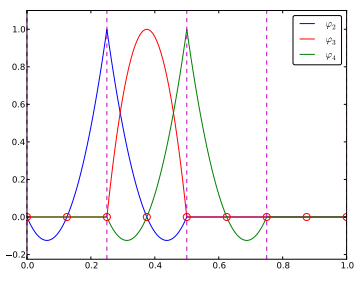
\includegraphics[width=0.7\linewidth]{img_18}
	\caption{Illustration of the piecewise quadratic basis functions associated
		with nodes in element 1.}
	\label{fig:img_18}
\end{figure}

\noindent Since $A_{i, j}$ is the integral of $\varphi_{i} \varphi_{j}$ it means that \textit{most of the elements in the coefficient matrix will be zero}. We will come back to these properties and use them actively in computations to save memory and CPU time.

We let each element have $d+1$ nodes, resulting in local Lagrange polynomials of degree $d$. It is not a requirement to have the same $d$ value in each element, but for now we will assume so.
\section[Example on piecewise quadratic finite element functions]{Example on piecewise quadratic finite element functions}
\label{sec:sec_3_3}
\noindent Figure 18 illustrates how piecewise quadratic basis functions can look like $(d=2)$. We work with the domain $\Omega=[0,1]$ divided into four equal-sized elements, each having three nodes. The nodes and elements lists in this particular example become
\begin{lstlisting}[numbers=none]
nodes = [0, 0.125, 0.25, 0.375, 0.5, 0.625, 0.75, 0.875, 1.0]
elements = [[0, 1, 2], [2, 3, 4], [4, 5, 6], [6, 7, 8]]	
\end{lstlisting}
Figure \hyperref[fig:img_19]{19} sketches the mesh and the numbering. Nodes are marked with circles on the $x$ axis and element boundaries are marked with vertical dashed lines in Figure \hyperref[fig:img_18]{18}.

Let us explain in detail how the basis functions are constructed according to the principles. Consider element number 1 in Figure \hyperref[fig:img_18]{18} $, \Omega^{(1)}=[0.25,0.5]$,
\begin{figure}[H]
	\centering
	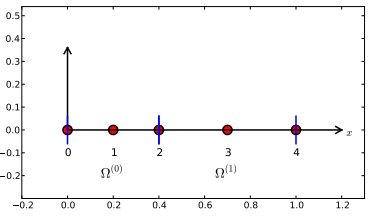
\includegraphics[width=0.7\linewidth]{img_19}
	\caption{Sketch of mesh with 4 elements and 3 nodes per element.}
	\label{fig:img_19}
\end{figure}
\noindent with local nodes 0,1 , and 2 corresponding to global nodes 2 , 3 , and 4 . The coordinates of these nodes are $0.25,0.375$, and $0.5$, respectively. We define three Lagrange polynomials on this element:
\begin{enumerate}
	\item The polynomial that is 1 at local node $1(x=0.375$, global node 3 ) makes up the basis function $\varphi_{3}(x)$ over this element, with $\varphi_{3}(x)=0$ outside the element.
	\item The Lagrange polynomial that is 1 at local node 0 is the "right part" of the global basis function $\varphi_{2}(x)$. The "left part" of $\varphi_{2}(x)$ consists of a Lagrange polynomial associated with local node 2 in the neighboring element $\Omega^{(0)}=[0,0.25]$.
	\item Finally, the polynomial that is 1 at local node 2 (global node 4 ) is the "left part" of the global basis function $\varphi_{4}(x)$. The "right part" comes from the Lagrange polynomial that is 1 at local node 0 in the neighboring element $\Omega^{(2)}=[0.5,0.75]$.
\end{enumerate}	

\noindent As mentioned earlier, any global basis function $\varphi_{i}(x)$ is zero on elements that do not contain the node with global node number $i$.

The other global functions associated with internal nodes, $\varphi_{1}, \varphi_{5}$, and $\varphi_{7}$, are all of the same shape as the drawn $\varphi_{3}$, while the global basis functions associated with shared nodes also have the same shape, provided the elements are of the same length.

\section[Example on piecewise linear finite element functions]{Example on piecewise linear finite element functions}
\label{sec:sec_3_4}
Figure \hyperref[fig:img_20]{20} shows piecewise linear basis functions $(d=1)$. Also here we have four elements on $\Omega=[0,1]$. Consider the element $\Omega^{(1)}=[0.25,0.5]$. Now there are no internal nodes in the elements so that all basis functions are associated with nodes at the element boundaries and hence made up of two Lagrange
\begin{figure}[H]
	\centering
	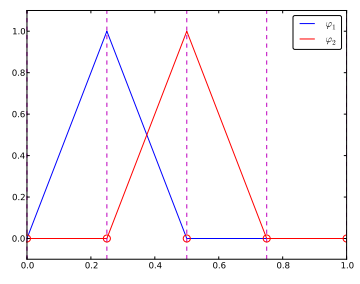
\includegraphics[width=0.7\linewidth]{img_20}
	\caption{Illustration of the piecewise linear basis functions associated with
		nodes in element 1.}
	\label{fig:img_20}
\end{figure}

\noindent polynomials from neighboring elements. For example, $\varphi_{1}(x)$ results from the Lagrange polynomial in element 0 that is 1 at local node 1 and 0 at local node 0 , combined with the Lagrange polynomial in element 1 that is 1 at local node 0 and 0 at local node 1 . The other basis functions are constructed similarly.

Explicit mathematical formulas are needed for $\varphi_{i}(x)$ in computations. In the piecewise linear case, one can show that
\begin{equation}\label{eqa53}
	\varphi_{i}(x)= \begin{cases}0, & x<x_{i-1}, \\ \left(x-x_{i-1}\right) /\left(x_{i}-x_{i-1}\right), & x_{i-1} \leq x<x_{i}, \\ 1-\left(x-x_{i}\right) /\left(x_{i+1}-x_{i}\right), & x_{i} \leq x<x_{i+1}, \\ 0, & x \geq x_{i+1}.\end{cases}
\end{equation}
Here, $x_{j}, j=i-1, i, i+1$, denotes the coordinate of node $j$. For elements of equal length $h$ the formulas can be simplified to
\begin{equation}\label{eqa54}
	\varphi_{i}(x)= \begin{cases}0, & x<x_{i-1}, \\ \left(x-x_{i-1}\right) / h, & x_{i-1} \leq x<x_{i}, \\ 1-\left(x-x_{i}\right) / h, & x_{i} \leq x<x_{i+1}, \\ 0, & x \geq x_{i+1}\end{cases}
\end{equation}
\section[Example on piecewise cubic finite element basis functions]{Example on piecewise cubic finite element basis functions}
\label{sec:sec_3_5}
Piecewise cubic basis functions can be defined by introducing four nodes per element. Figure \hyperref[fig:img_21]{21} shows examples on $\varphi_{Wi}(x)$, $i=3,4,5,6$, associated with element number 1. Note that $\varphi_{4}$ and $\varphi_{5}$ are nonzero on element number 1 , while $\varphi_{3}$ and $\varphi_{6}$ are made up of Lagrange polynomials on two neighboring elements.
\begin{figure}[H]
	\centering
	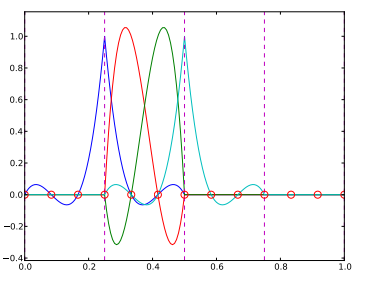
\includegraphics[width=0.7\linewidth]{img_21}
	\caption{Illustration of the piecewise cubic basis functions associated with
		nodes in element 1.}
	\label{fig:img_21}
\end{figure}

We see that all the piecewise linear basis functions have the same "hat" shape.
They are naturally referred to as \textit{hat functions}, also called \textit{chapeau functions.}
The piecewise quadratic functions in Figure \hyperref[fig:img_18]{18} are seen to be of two types.
"Rounded hats" associated with internal nodes in the elements and some more
"sombrero" shaped hats associated with element boundary nodes. Higher-order
basis functions also have hat-like shapes, but the functions have pronounced
oscillations in addition, as illustrated in Figure \hyperref[fig:img_21]{21}.

A common terminology is to speak about \textit{linear elements} as elements with two
local nodes associated with piecewise linear basis functions. Similarly, \textit{quadratic
elements} and \textit{cubic elements} refer to piecewise quadratic or cubic functions
over elements with three or four local nodes, respectively. Alternative names,
frequently used later, are P1 elements for linear elements, P2 for quadratic
elements, and so forth: Pd signifies degree d of the polynomial basis functions.

\section[Calculating the linear system]{Calculating the linear system}
\label{sec:sec_3_6}
The elements in the coefficient matrix and right-hand side are given by the formulas (\hyperref[eqa27]{27}) and (\hyperref[eqa28]{28}), but now the choice of $\psi_{i}$ is $\varphi_{i}$. Consider P1 elements where $\varphi_{i}(x)$ piecewise linear. Nodes and elements numbered consecutively from left to right in a uniformly partitioned mesh imply the nodes
$$
x_{i}=i h, \quad i=0, \ldots, N,
$$
and the elements
\begin{equation}\label{eqa55}
	\Omega^{(i)}=\left[x_{i}, x_{i+1}\right]=[i h,(i+1) h], \quad i=0, \ldots, N_{e}=N-1.
\end{equation}
We have in this case $N$ elements and $N+1$ nodes, and $\Omega=\left[x_{0}, x_{N}\right]$. The formula for $\varphi_{i}(x)$ is given by (\hyperref[eqa54]{54}) and a graphical illustration is provided in Figures \hyperref[fig:img_20]{20} and \hyperref[fig:img_23]{23} . First we clearly see from the figures the very important property $\varphi_{i}(x) \varphi_{j}(x) \neq 0$ if and only if $j=i-1, j=i$, or $j=i+1$, or alternatively expressed, if and only if $i$ and $j$ are nodes in the same element. Otherwise, $\varphi_{i}$ and $\varphi_{j}$ are too distant to have an overlap and consequently their product vanishes.
\begin{figure}[H]
	\centering
	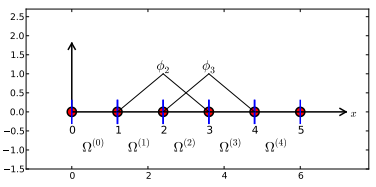
\includegraphics[width=0.7\linewidth]{img_22}
	\caption{Illustration of the piecewise linear basis functions corresponding to
		global node 2 and 3.}
	\label{fig:img_22}
\end{figure}

\noindent \textbf{Calculating a specific matrix entry.} Let us calculate the specific matrix entry $A_{2,3}=\int_{\Omega} \varphi_{2} \varphi_{3} \mathrm{~d} x$. Figure \hyperref[fig:img_22]{22} shows how $\varphi_{2}$ and $\varphi_{3}$ look like. We realize from this figure that the product $\varphi_{2} \varphi_{3} \neq 0$ only over element 2 , which contains node 2 and 3. The particular formulas for $\varphi_{2}(x)$ and $\varphi_{3}(x)$ on $\left[x_{2}, x_{3}\right]$ are found from (\hyperref[eqa54]{54}). The function $\varphi_{3}$ has positive slope over $\left[x_{2}, x_{3}\right]$ and corresponds to the interval $\left[x_{i-1}, x_{i}\right]$ in (\hyperref[eqa54]{54}). With $i=3$ we get
$$
\varphi_{3}(x)=\left(x-x_{2}\right) / h,
$$
while $\varphi_{2}(x)$ has negative slope over $\left[x_{2}, x_{3}\right]$ and corresponds to setting $i=2$ in (\hyperref[eqa54]{54}).

$$
\varphi_{2}(x)=1-\left(x-x_{2}\right) / h .
$$
We can now easily integrate,
$$
A_{2,3}=\int_{\Omega} \varphi_{2} \varphi_{3} \mathrm{~d} x=\int_{x_{2}}^{x_{3}}\left(1-\frac{x-x_{2}}{h}\right) \frac{x-x_{2}}{h} \mathrm{~d} x=\frac{h}{6}.
$$
The diagonal entry in the coefficient matrix becomes
$$
A_{2,2}=\int_{x_{1}}^{x_{2}}\left(\frac{x-x_{1}}{h}\right)^{2} \mathrm{~d} x+\int_{x_{2}}^{x_{3}}\left(1-\frac{x-x_{2}}{h}\right)^{2} \mathrm{~d} x=\frac{h}{3}.
$$
The entry $A_{2,1}$ has an the integral that is geometrically similar to the situation in Figure \hyperref[fig:img_22]{22}, so we get $A_{2,1}=h / 6$.
\bigbreak
\noindent \textbf{Calculating a general row in the matrix.} We can now generalize the calculation of matrix entries to a general row number $i$. The entry $A_{i, i-1}=$ $\int_{\Omega} \varphi_{i} \varphi_{i-1} \mathrm{~d} x$ involves hat functions as depicted in Figure \hyperref[fig:img_23]{23} . Since the integral is geometrically identical to the situation with specific nodes 2 and 3 , we realize that $A_{i, i-1}=A_{i, i+1}=h / 6$ and $A_{i, i}=2 h / 3$. However, we can compute the integral directly too:
$$
\begin{aligned}
	A_{i, i-1} &=\int_{\Omega} \varphi_{i} \varphi_{i-1} \mathrm{~d} x \\
	&=\underbrace{\int_{x_{i-2}}^{x_{i-1}} \varphi_{i} \varphi_{i-1} \mathrm{~d} x}_{\varphi_{i}=0}+\int_{x_{i-1}}^{x_{i}} \varphi_{i} \varphi_{i-1} \mathrm{~d} x+\underbrace{\int_{x_{i}}^{x_{i+1}} \varphi_{i} \varphi_{i-1} \mathrm{~d} x}_{\varphi_{i-1}=0} \\
	&=\int_{x_{i-1}}^{x_{i}} \underbrace{\left(\frac{x-x_{i}}{h}\right)}_{\varphi_{i}(x)} \underbrace{\left(1-\frac{x-x_{i-1}}{h}\right)}_{\varphi_{i-1}(x)} \mathrm{d} x=\frac{h}{6}.
\end{aligned}
$$
The particular formulas for $\varphi_{i-1}(x)$ and $\varphi_{i}(x)$ on $\left[x_{i-1}, x_{i}\right]$ are found from (\hyperref[eqa54]{54}): $\varphi_{i}$ is the linear function with positive slope, corresponding to the interval $\left[x_{i-1}, x_{i}\right]$ in (\hyperref[eqa54]{54}), while $\phi_{i-1}$ has a negative slope so the definition in interval $\left[x_{i}, x_{i+1}\right]$ in (\hyperref[eqa54]{54}) must be used. (The appearance of $i$ in (\hyperref[eqa54]{54}) and the integral might be confusing, as we speak about two different $i$ indices.)

The first and last row of the coefficient matrix lead to slightly different integrals:
$$
A_{0,0}=\int_{\Omega} \varphi_{0}^{2} \mathrm{~d} x=\int_{x_{0}}^{x_{1}}\left(1-\frac{x-x_{0}}{h}\right)^{2} \mathrm{~d} x=\frac{h}{3}.
$$
Similarly, $A_{N, N}$ involves an integral over only one element and equals hence $h / 3$. The general formula for $b_{i}$, see Figure \hyperref[fig:img_24]{24}, is now easy to set up
\begin{figure}[H]
	\centering
	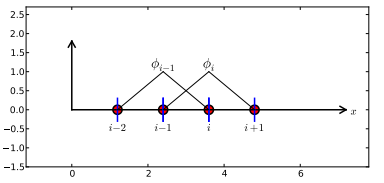
\includegraphics[width=0.7\linewidth]{img_23}
	\caption{Illustration of two neighboring linear (hat) functions with general
		node numbers.}
	\label{fig:img_23}
\end{figure}
\begin{figure}[H]
	\centering
	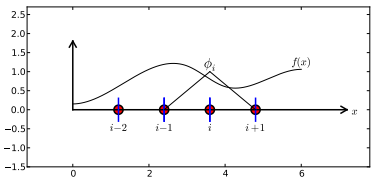
\includegraphics[width=0.7\linewidth]{img_24}
	\caption{Right-hand side integral with the product of a basis function and
		the given function to approximate.}
	\label{fig:img_24}
\end{figure}
\begin{equation}\label{eqa56}
	b_{i}=\int_{\Omega} \varphi_{i}(x) f(x) \mathrm{d} x=\int_{x_{i-1}}^{x_{i}} \frac{x-x_{i-1}}{h} f(x) \mathrm{d} x+\int_{x_{i}}^{x_{i+1}}\left(1-\frac{x-x_{i}}{h}\right) f(x) \mathrm{d} x.
\end{equation}
We need a specific $f(x)$ function to compute these integrals. With two equal-sized elements in $\Omega=[0,1]$ and $f(x)=x(1-x)$, one gets
$$
A=\frac{h}{6}\left(\begin{array}{ccc}
	2 & 1 & 0 \\
	1 & 4 & 1 \\
	0 & 1 & 2
\end{array}\right), \quad b=\frac{h^{2}}{12}\left(\begin{array}{c}
	2-3 h \\
	12-14 h \\
	10-17 h
\end{array}\right)
$$
The solution becomes
$$
c_{0}=\frac{h^{2}}{6}, \quad c_{1}=h-\frac{5}{6} h^{2}, \quad c_{2}=2 h-\frac{23}{6} h^{2}.
$$
The resulting function
$$
u(x)=c_{0} \varphi_{0}(x)+c_{1} \varphi_{1}(x)+c_{2} \varphi_{2}(x)
$$
is displayed in Figure \hyperref[fig:img_25]{25} (left). Doubling the number of elements to four leads to the improved approximation in the right part of Figure \hyperref[fig:img_25]{25} .
\begin{figure}[H]
	\centering
	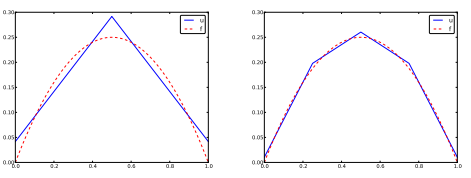
\includegraphics[width=0.7\linewidth]{img_25}
	\caption{Least squares approximation of a parabola using 2 (left) and 4
		(right) P1 elements.}
	\label{fig:img_25}
\end{figure}

\section[Assembly of elementwise computations]{Assembly of elementwise computations}
\label{sec:sec_3_7}
The integrals above are naturally split into integrals over individual elements since the formulas change with the elements. This idea of splitting the integral is fundamental in all practical implementations of the finite element method.
Let us split the integral over $\Omega$ into a sum of contributions from each element:
\begin{equation}\label{eqa57}
	A_{i, j}=\int_{\Omega} \rho_{i} \rho_{j} \mathrm{~d} x=\sum_{e} A_{i, j}^{(e)}, \quad A_{i, j}^{(e)}=\int_{\Omega^{(e)}} \rho_{i} \rho_{j} \mathrm{~d} x.
\end{equation}
Now, $A_{i, j}^{(e)} \neq 0$ if and only if $i$ and $j$ are nodes in element $e$. Introduce $i=q(e, r)$ as the mapping of local node number $r$ in element $e$ to the global node number $i$. This is just a short mathematical notation for the expression $i=e l$ ements [e] [r] in a program. Let $r$ and $s$ be the local node numbers corresponding to the global node numbers $i=q(e, r)$ and $j=q(e, s)$. With $d$ nodes per element, all the nonzero elements in $A_{i, j}^{(e)}$ arise from the integrals involving basis functions with indices corresponding to the global node numbers in element number $e$ :
$$
\int_{\Omega^{(e)}} \varphi_{q(e, r)} \varphi_{q(e, s)} \mathrm{d} x, \quad r, s=0, \ldots, d .
$$
These contributions can be collected in a $(d+1) \times(d+1)$ matrix known as the \textit{element matrix}. Let $I_{d}=\{0, \ldots, d\}$ be the valid indices of $r$ and $s$. We introduce the notation
$$
\tilde{A}^{(e)}=\left\{\tilde{A}_{r, s}^{(e)}\right\}, \quad r, s \in I_{d},
$$
for the element matrix. For the case $d=2$ we have
$$
\tilde{A}^{(e)}=\left[\begin{array}{ccc}
	\tilde{A}_{0,0}^{(e)} & \tilde{A}_{0,1}^{(e)} & \tilde{A}_{0,2}^{(e)} \\
	\tilde{A}_{1,0}^{(e)} & \tilde{A}_{1,1}^{(e)} & \tilde{A}_{1,2}^{(e)} \\
	\tilde{A}_{2,0}^{(e)} & \tilde{A}_{2,1}^{(e)} & \tilde{A}_{2,2}^{(e)}
\end{array}\right] .
$$
Given the numbers $\tilde{A}_{r, s}^{(e)}$, we should according to (\hyperref[eqa57]{57}) add the contributions to the global coefficient matrix by
\begin{equation}\label{eqa58}
	A_{q(e, r), q(e, s)}:=A_{q(e, r), q(e, s)}+\tilde{A}_{r, s}^{(e)}, \quad r, s \in I_{d} .
\end{equation}

This process of adding in elementwise contributions to the global matrix is called \textit{finite element assembly} or simply \textit{assembly}. Figure \hyperref[fig:img_26]{26} illustrates how element matrices for elements with two nodes are added into the global matrix. More specifically, the figure shows how the element matrix associated with elements 1 and 2 assembled, assuming that global nodes are numbered from left to right in the domain. With regularly numbered P3 elements, where the element matrices have size $4 \times 4$, the assembly of elements 1 and 2 are sketched in Figure \hyperref[fig:img_27]{27}.
\begin{figure}[H]
	\centering
	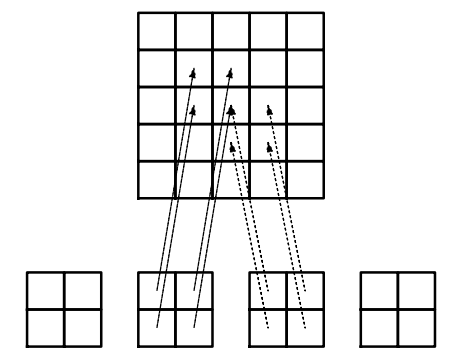
\includegraphics[width=0.7\linewidth]{img_26}
	\caption{Illustration of matrix assembly: regularly numbered P1 elements.}
	\label{fig:img_26}
\end{figure}

After assembly of element matrices corresponding to regularly numbered
elements and nodes are understood, it is wise to study the assembly process for
irregularly numbered elements and nodes. Figure \hyperref[fig:img_17]{17} shows a mesh where the
elements array, or q(e, r) mapping in mathematical notation, is given as
\begin{figure}[H]
	\centering
	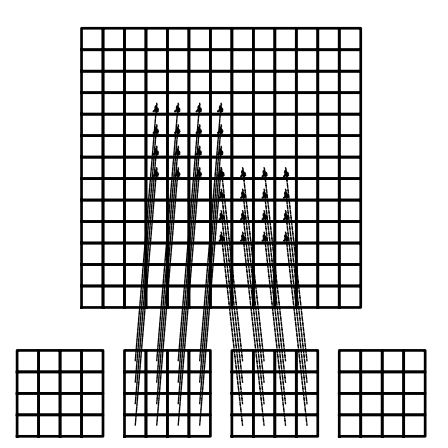
\includegraphics[width=0.7\linewidth]{img_27}
	\caption{Illustration of matrix assembly: regularly numbered P3 elements.}
	\label{fig:img_27}
\end{figure}

\begin{lstlisting}[numbers=none]
elements = [[2, 1], [4, 5], [0, 4], [3, 0], [5, 2]
\end{lstlisting}
The associated assembly of element matrices 1 and 2 is sketched in Figure \hyperref[fig:img_28]{28}. 

These three assembly processes can also be \href{http://hplgit.github.io/INF5620/doc/pub/mov-fem/fe_assembly.html}{animated.}


The right-hand side of the linear system is also computed elementwise:
\begin{equation}\label{eqa59}
	b_{i}=\int_{\Omega} f(x) \varphi_{i}(x) \mathrm{d} x=\sum_{e} b_{i}^{(e)}, \quad b_{i}^{(e)}=\int_{\Omega^{(e)}} f(x) \varphi_{i}(x) \mathrm{d} x.
\end{equation}
We observe that $b_{i}^{(e)} \neq 0$ if and only if global node $i$ is a node in element $e$. With $d$ nodes per element we can collect the $d+1$ nonzero contributions $b_{i}^{(e)}$, for $i=q(e, r), r \in I_{d}$, in an \textit{element vector}
$$
\tilde{b}_{r}^{(e)}=\left\{\tilde{b}_{r}^{(e)}\right\}, \quad r \in I_{d} .
$$
These contributions are added to the global right-hand side by an assembly process similar to that for the element matrices:
\begin{figure}[H]
	\centering
	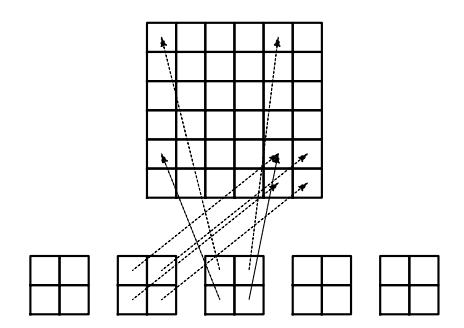
\includegraphics[width=0.7\linewidth]{img_28}
	\caption{Illustration of matrix assembly: irregularly numbered P1 elements.}
	\label{fig:img_28}
\end{figure}
\begin{equation}\label{eqa60}
	b_{q(e, r)}:=b_{q(e, r)}+\tilde{b}_{r}^{(e)}, \quad r \in I_{d}.
\end{equation}
\section[Mapping to a reference element]{Mapping to a reference element}
\label{sec:sec_3_8}
Instead of computing the integrals
$$
\tilde{A}_{r, s}^{(e)}=\int_{\Omega^{(e)}} \varphi_{q(e, r)}(x) \varphi_{q(e, s)}(x) \mathrm{d} x
$$
over some element $\Omega^{(e)}=\left[x_{L}, x_{R}\right]$, it is convenient to map the element domain $\left[x_{L}, x_{R}\right]$ to a standardized reference element domain $[-1,1]$. (We have now introduced $x_{L}$ and $x_{R}$ as the left and right boundary points of an arbitrary element. With a natural, regular numbering of nodes and elements from left to right through the domain, we have $x_{L}=x_{e}$ and $x_{R}=x_{e+1}$ for $\mathrm{P} 1$ elements.)

Let $X \in[-1,1]$ be the coordinate in the reference element. A linear or \textit{affine mapping} from $X$ to $x$ reads
\begin{equation}\label{eqa61}
	x=\frac{1}{2}\left(x_{L}+x_{R}\right)+\frac{1}{2}\left(x_{R}-x_{L}\right) X.
\end{equation}
This relation can alternatively be expressed by
\begin{equation}\label{eqa62}
	x=x_{m}+\frac{1}{2} h X,
\end{equation}
where we have introduced the element midpoint $x_{m}=\left(x_{L}+x_{R}\right) / 2$ and the element length $h=x_{R}-x_{L}$.

Integrating on the reference element is a matter of just changing the integration variable from $x$ to $X$. Let
\begin{equation}\label{eqa63}
	\tilde{\varphi}_{r}(X)=\varphi_{q(e, r)}(x(X))
\end{equation}
be the basis function associated with local node number $r$ in the reference element. The integral transformation reads
\begin{equation}\label{eqa64}
	\tilde{A}_{r, s}^{(e)}=\int_{\Omega^{(e)}} \varphi_{q(e, r)}(x) \varphi_{q(e, s)}(x) \mathrm{d} x=\int_{-1}^{1} \tilde{\varphi}_{r}(X) \tilde{\varphi}_{s}(X) \frac{d x}{d X} \mathrm{~d} X.
\end{equation}
The stretch factor $d x / d X$ between the $x$ and $X$ coordinates becomes the determinant of the Jacobian matrix of the mapping between the coordinate systems in $2 \mathrm{D}$ and 3D. To obtain a uniform notation for $1 \mathrm{D}, 2 \mathrm{D}$, and 3D problems we therefore replace $d x / d X$ by det $J$ already now. In $1 \mathrm{D}$, $\operatorname{det} J=d x / d X=h / 2$. The integration over the reference element is then written as
\begin{equation}\label{eqa65}
	\tilde{A}_{r, s}^{(e)}=\int_{-1}^{1} \tilde{\varphi}_{r}(X) \tilde{\varphi}_{s}(X) \operatorname{det} J d X.
\end{equation}
The corresponding formula for the element vector entries becomes
\begin{equation}\label{eqa66}
	\tilde{b}_{r}^{(e)}=\int_{\Omega^{(e)}} f(x) \varphi_{q(e, r)}(x) d x=\int_{-1}^{1} f(x(X)) \tilde{\varphi}_{r}(X) \operatorname{det} J d X.
\end{equation}

Since we from now on will work in the reference element, we need explicit mathematical formulas for the basis functions $\varphi_{i}(x)$ in the reference element only, i.e., we only need to specify formulas for $\tilde{\varphi}_{r}(X)$. This is a very convenient simplification compared to specifying piecewise polynomials in the physical domain.

The $\tilde{\varphi}_{r}(x)$ functions are simply the Lagrange polynomials defined through the local nodes in the reference element. For $d=1$ and two nodes per element, we have the linear Lagrange polynomials
\begin{equation}\label{eqa67}
	\tilde{\varphi}_{0}(X) =\frac{1}{2}(1-X)
\end{equation}
\begin{equation}\label{eqa68}
	\tilde{\varphi}_{1}(X) =\frac{1}{2}(1+X)
\end{equation}
Quadratic polynomials, $d=2$, have the formulas
\begin{equation}\label{eqa69}
	\tilde{\varphi}_{0}(X) =\frac{1}{2}(X-1) X
\end{equation}
\begin{equation}\label{eqa70}
	\tilde{\varphi}_{1}(X) =1-X^{2}
\end{equation}
\begin{equation}\label{eqa71}
	\tilde{\varphi}_{2}(X) =\frac{1}{2}(X+1)X
\end{equation}
In general,
\begin{equation}\label{eqa72}
	\tilde{\varphi}_{r}(X)=\prod_{s=0, s \neq r}^{d} \frac{X-X_{(s)}}{X_{(r)}-X_{(s)}},
\end{equation}
where $X_{(0)}, \ldots, X_{(d)}$ are the coordinates of the local nodes in the reference element. These are normally uniformly spaced: $X_{(r)}=-1+2 r / d, r \in I_{d}$.
\begin{mybox}
	\textbf{Why reference elements?}
	
	\noindent The great advantage of using reference elements is that the formulas for the basis functions, $\tilde{\varphi}_{r}(X)$, are the same for all elements and independent of the element geometry (length and location in the mesh). The geometric information is "factored out" in the simple mapping formula and the associated det $J$ quantity, but this information is (here taken as) the same for element types. Also, the integration domain is the same for all elements.
\end{mybox}


\section[Example: Integration over a reference element]{Example: Integration over a reference element}
\label{sec:sec_3_9}
\noindent To illustrate the concepts from the previous section in a specific example, we now consider calculation of the element matrix and vector for a specific choice of $d$ and $f(x)$. A simple choice is $d=1$ (P1 elements) and $f(x)=x(1-x)$ on $\Omega=[0,1]$. We have the general expressions (\hyperref[eqa65]{65}) and (\hyperref[eqa66]{66}) for $\tilde{A}_{r, s}^{(e)}$ and $\tilde{b}_{r}^{(e)}$. Writing these out for the choices (\hyperref[eqa67]{67}) and (\hyperref[eqa68]{68}), and using that $\operatorname{det} J=h / 2$, we can do the following calculations of the element matrix entries:
\begin{equation}\label{eqa73}
	\begin{aligned}
		\tilde{A}_{0,0}^{(e)} &=\int_{-1}^{1} \tilde{\varphi}_{0}(X) \tilde{\varphi}_{0}(X) \frac{h}{2} d X \\
		&=\int_{-1}^{1} \frac{1}{2}(1-X) \frac{1}{2}(1-X) \frac{h}{2} d X=\frac{h}{8} \int_{-1}^{1}(1-X)^{2} d X=\frac{h}{3},
	\end{aligned}
\end{equation}
\begin{equation}\label{eqa74}
	\begin{aligned}
		\tilde{A}_{1,0}^{(e)} &=\int_{-1}^{1} \tilde{\varphi}_{1}(X) \tilde{\varphi}_{0}(X) \frac{h}{2} d X \\
		&=\int_{-1}^{1} \frac{1}{2}(1+X) \frac{1}{2}(1-X) \frac{h}{2} d X=\frac{h}{8} \int_{-1}^{1}\left(1-X^{2}\right) d X=\frac{h}{6},
	\end{aligned}
\end{equation}
\begin{equation}\label{eqa75}
	\tilde{A}_{0,1}^{(e)} =\tilde{A}_{1,0}^{(e)},
\end{equation}
\begin{equation}\label{eqa76}
	\begin{aligned}
		\tilde{A}_{1,1}^{(e)} &=\int_{-1}^{1} \tilde{\varphi}_{1}(X) \tilde{\varphi}_{1}(X) \frac{h}{2} d X \\
		&=\int_{-1}^{1} \frac{1}{2}(1+X) \frac{1}{2}(1+X) \frac{h}{2} d X=\frac{h}{8} \int_{-1}^{1}(1+X)^{2} d X=\frac{h}{3}.
	\end{aligned}
\end{equation}
The corresponding entries in the element vector becomes
\begin{equation}\label{eqa77}
	\begin{aligned}
		\tilde{b}_{0}^{(e)} &=\int_{-1}^{1} f(x(X)) \tilde{\varphi}_{0}(X) \frac{h}{2} d X \\
		&=\int_{-1}^{1}\left(x_{m}+\frac{1}{2} h X\right)\left(1-\left(x_{m}+\frac{1}{2} h X\right)\right) \frac{1}{2}(1-X) \frac{h}{2} d X \\
		&=-\frac{1}{24} h^{3}+\frac{1}{6} h^{2} x_{m}-\frac{1}{12} h^{2}-\frac{1}{2} h x_{m}^{2}+\frac{1}{2} h x_{m}.
	\end{aligned}
\end{equation}
\begin{equation}\label{eqa78}
	\begin{aligned}
		\tilde{b}_{1}^{(e)} &=\int_{-1}^{1} f(x(X)) \tilde{\varphi}_{1}(X) \frac{h}{2} d X \\
		&=\int_{-1}^{1}\left(x_{m}+\frac{1}{2} h X\right)\left(1-\left(x_{m}+\frac{1}{2} h X\right)\right) \frac{1}{2}(1+X) \frac{h}{2} d X \\
		&=-\frac{1}{24} h^{3}-\frac{1}{6} h^{2} x_{m}+\frac{1}{12} h^{2}-\frac{1}{2} h x_{m}^{2}+\frac{1}{2} h x_{m}.
	\end{aligned}
\end{equation}
In the last two expressions we have used the element midpoint $x_{m}$.

Integration of lower-degree polynomials above is tedious, and higher-degree polynomials involve very much more algebra, but sympy may help. For example, we can easily calculate (\hyperref[eqa73]{73}), (\hyperref[eqa73]{73}) and (\hyperref[eqa77]{77}) by
\begin{lstlisting}[numbers=none]
>>> import sympy as sp
>>> x, x_m, h, X = sp.symbols('x x_m h X')
>>> sp.integrate(h/8*(1-X)**2, (X, -1, 1))
h/3
>>> sp.integrate(h/8*(1+X)*(1-X), (X, -1, 1))
h/6
>>> x = x_m + h/2*X
>>> b_0 = sp.integrate(h/4*x*(1-x)*(1-X), (X, -1, 1))
>>> print b_0
-h**3/24 + h**2*x_m/6 - h**2/12 - h*x_m**2/2 + h*x_m/2	
\end{lstlisting}
For inclusion of formulas in documents (like the present one), sympy can print
expressions in LATEX format:
\begin{lstlisting}[numbers=none]
>>> print sp.latex(b_0, mode='plain')
- \frac{1}{24} h^{3} + \frac{1}{6} h^{2} x_{m}
- \frac{1}{12} h^{2} - \half h x_{m}^{2}
+ \half h x_{m
\end{lstlisting}
\chapter{Implementation}
\label{chap:chap_4}
\noindent Based on the experience from the previous example, it makes sense to write
some code to automate the analytical integration process for any choice of finite
element basis functions. In addition, we can automate the assembly process
and linear system solution. Appropriate functions for this purpose document
all details of all steps in the finite element computations and can found in the
module file \href{https://github.com/hplgit/INF5620/blob/master/src/fem/fe_approx1D.py}{fe\textunderscore approx1D.py.} The key steps in the computational machinery are
now explained in detail in terms of code and text.
\section[Integration]{Integration}
\label{sec:sec_4_1}
First we need a Python function for defining $\tilde{\varphi}_{r}(X)$ in terms of a Lagrange polynomial of degree $d$ :
\begin{lstlisting}[numbers=none]
import sympy as sp
import numpy as np
def phi_r(r, X, d):
	if isinstance(X, sp.Symbol):
		h = sp.Rational(1, d) # node spacing
		nodes = [2*i*h - 1 for i in range(d+1)]
	else:
		# assume X is numeric: use floats for nodes
		nodes = np.linspace(-1, 1, d+1)
	return Lagrange_polynomial(X, r, nodes)
	
def Lagrange_polynomial(x, i, points):
	p = 1
	for k in range(len(points)):
		if k != i:
			p *= (x - points[k])/(points[i] - points[k])
	return p	
\end{lstlisting}
Observe how we construct the phi\textunderscore r function to be a symbolic expression for $\tilde{\varphi}_{r}(X)$ if $\mathrm{X}$ is a Symbol object from sympy. Otherwise, we assume that $\mathrm{X}$ is a float object and compute the corresponding floating-point value of $\ddot{\varphi}_{r}(X)$. Recall that the Lagrange\textunderscore polynomial function, here simply copied from Section \hyperref[sec:sec_2_7]{2.7}, works with both symbolic and numeric variables.

The complete basis $\tilde{\varphi}_{0}(X), \ldots, \tilde{\varphi}_{d}(X)$ on the reference element, represented as a list of symbolic expressions, is constructed by
\begin{lstlisting}[numbers=none]
def basis(d=1):
	X = sp.Symbol('X')
	phi = [phi_r(r, X, d) for r in range(d+1)]
	return phi	
\end{lstlisting}
Now we are in a position to write the function for computing the element matrix:
\begin{lstlisting}[numbers=none]
def element_matrix(phi, Omega_e, symbolic=True):
	n = len(phi)
	A_e = sp.zeros((n, n))
	X = sp.Symbol('X')
	if symbolic:
		h = sp.Symbol('h')
	else:
		h = Omega_e[1] - Omega_e[0]
	detJ = h/2 # dx/dX
	for r in range(n):
		for s in range(r, n):
			A_e[r,s] = sp.integrate(phi[r]*phi[s]*detJ, (X, -1, 1))
			A_e[s,r] = A_e[r,s]
	return A_e	
\end{lstlisting}
In the symbolic case (symbolic is True), we introduce the element length as
a symbol h in the computations. Otherwise, the real numerical value of the element interval Omega\textunderscore e is used and the final matrix elements are numbers, not
symbols. This functionality can be demonstrated:
\begin{lstlisting}[numbers=none]
>>> from fe_approx1D import *
>>> phi = basis(d=1)
>>> phi
[1/2 - X/2, 1/2 + X/2]
>>> element_matrix(phi, Omega_e=[0.1, 0.2], symbolic=True)
[h/3, h/6]
[h/6, h/3]
>>> element_matrix(phi, Omega_e=[0.1, 0.2], symbolic=False)
[0.0333333333333333, 0.0166666666666667]
[0.0166666666666667, 0.0333333333333333]	
\end{lstlisting}
The computation of the element vector is done by a similar procedure:
\begin{lstlisting}[numbers=none]
def element_vector(f, phi, Omega_e, symbolic=True):
	n = len(phi)
	b_e = sp.zeros((n, 1))
	# Make f a function of X
	X = sp.Symbol('X')
	if symbolic:
		h = sp.Symbol('h')
	else:
	h = Omega_e[1] - Omega_e[0]
	x = (Omega_e[0] + Omega_e[1])/2 + h/2*X # mapping
	f = f.subs('x', x) # substitute mapping formula for x
	detJ = h/2 # dx/dX
	for r in range(n):
		b_e[r] = sp.integrate(f*phi[r]*detJ, (X, -1, 1))
	return b_e	
\end{lstlisting}
Here we need to replace the symbol $x$ in the expression for $f$ by the mapping formula such that $f$ can be integrated in terms of $X$, cf. the formula $\tilde{b}_{r}^{(e)}=$ $\int_{-1}^{1} f(x(X)) \tilde{\varphi}_{r}(X) \frac{h}{2} d X$.

The integration in the element matrix function involves only products of polynomials, which sympy can easily deal with, but for the right-hand side sympy may face difficulties with certain types of expressions $f$. The result of the integral is then an Integral object and not a number or expression as when symbolic integration is successful. It may therefore be wise to introduce a fallback on numerical integration. The symbolic integration can also take much time before an unsuccessful conclusion so we may also introduce a parameter symbolic and set it to False to avoid symbolic integration:
\begin{lstlisting}[numbers=none]
def element_vector(f, phi, Omega_e, symbolic=True):
		...
		if symbolic:
			I = sp.integrate(f*phi[r]*detJ, (X, -1, 1))
		if not symbolic or isinstance(I, sp.Integral):
			h = Omega_e[1] - Omega_e[0] # Ensure h is numerical
			detJ = h/2
			integrand = sp.lambdify([X], f*phi[r]*detJ)
			I = sp.mpmath.quad(integrand, [-1, 1])
		b_e[r] = I
		...
\end{lstlisting}
Numerical integration requires that the symbolic integrand is converted to a plain
Python function (integrand) and that the element length h is a real number.
\section[Linear system assembly and solution]{Linear system assembly and solution}
\label{sec:sec_4_2}
The complete algorithm for computing and assembling the elementwise contributions takes the following form
\begin{lstlisting}[numbers=none]
def assemble(nodes, elements, phi, f, symbolic=True):
	N_n, N_e = len(nodes), len(elements)
	if symbolic:
		A = sp.zeros((N_n, N_n))
		b = sp.zeros((N_n, 1)) # note: (N_n, 1) matrix
	else:
		A = np.zeros((N_n, N_n))
		b = np.zeros(N_n)
	for e in range(N_e):
		Omega_e = [nodes[elements[e][0]], nodes[elements[e][-1]]]
		
		A_e = element_matrix(phi, Omega_e, symbolic)
		b_e = element_vector(f, phi, Omega_e, symbolic)
		
		for r in range(len(elements[e])):
			for s in range(len(elements[e])):
				A[elements[e][r],elements[e][s]] += A_e[r,s]
			b[elements[e][r]] += b_e[r]
	return A, b	
\end{lstlisting}
The nodes and elements variables represent the finite element mesh as explained earlier.

Given the coefficient matrix $\mathrm{A}$ and the right-hand side $\mathrm{b}$, we can compute the coefficients $\left\{c_{i}\right\}_{i \in \mathcal{I}_{s}}$ in the expansion $u(x)=\sum_{j} c_{j} \varphi_{j}$ as the solution vector $c$ of the linear system:
\begin{lstlisting}[numbers=none]
if symbolic:
	c = A.LUsolve(b)
else:
	c = np.linalg.solve(A, b)
\end{lstlisting}
When A and b are sympy arrays, the solution procedure implied by A.LUsolve is
symbolic. Otherwise, A and b are numpy arrays and a standard numerical solver
is called. The symbolic version is suited for small problems only (small N values)
since the calculation time becomes prohibitively large otherwise. Normally, the
symbolic integration will be more time consuming in small problems than the
symbolic solution of the linear system.
\section[Example on computing symbolic approximations]{Example on computing symbolic approximations}
\label{sec:sec_4_3}
We can exemplify the use of assemble on the computational case from Section \hyperref[sec:sec_3_6]{3.6} with two P1 clcments (lincar basis functions) on the domain $\Omega=[0,1]$. Let us first work with a symbolic element length:
\begin{lstlisting}[numbers=none]
>>> h, x = sp.symbols('h x')
>>> nodes = [0, h, 2*h]
>>> elements = [[0, 1], [1, 2]]
>>> phi = basis(d=1)
>>> f = x*(1-x)
>>> A, b = assemble(nodes, elements, phi, f, symbolic=True)
>>> A
[h/3, h/6, 0]
[h/6, 2*h/3, h/6]
[ 0, h/6, h/3]
>>> b
[ h**2/6 - h**3/12]
[ h**2 - 7*h**3/6]
[5*h**2/6 - 17*h**3/12]
>>> c = A.LUsolve(b)
>>> c
[ h**2/6]
[12*(7*h**2/12 - 35*h**3/72)/(7*h)]
[ 7*(4*h**2/7 - 23*h**3/21)/(2*h)]	
\end{lstlisting}
\section[Comparison with finite elements and interpolation/- collocation]{Comparison with finite elements and interpolation/- collocation}
\label{sec:sec_4_4}
We may, for comparison, compute the c vector corresponding to an interpolation/collocation method with finite element basis functions. Choosing the nodes as points, the principle is
$$
u\left(x_{i}\right)=\sum_{j \in \mathcal{I}_{s}} c_{j} \varphi_{j}\left(x_{i}\right)=f\left(x_{i}\right), \quad i \in \mathcal{I}_{s}.
$$
The coefficient matrix $A_{i, j}=\varphi_{j}\left(x_{i}\right)$ becomes the identity matrix because basis function number $j$ vanishes at all nodes, except node $j: \varphi_{j}\left(x_{i}=\delta_{i j}\right.$. Therefore, $c_{i}=f\left(x_{i}\right.$.

The associated sympy calculations are
\begin{lstlisting}[numbers=none]
>>> fn = sp.lambdify([x], f)
>>> c = [fn(xc) for xc in nodes]
>>> c
[0, h*(1 - h), 2*h*(1 - 2*h)]
\end{lstlisting}
These expressions are much simpler than those based on least squares or projection in combination with finite element basis functions.
\section[Example on computing numerical approximations]{Example on computing numerical approximations}
\label{sec:sec_4_5}
The numerical computations corresponding to the symbolic ones in Section \hyperref[sec:sec_4_3]{4.3},
and still done by sympy and the assemble function, go as follows:
\begin{lstlisting}[numbers=none]
>>> nodes = [0, 0.5, 1]
>>> elements = [[0, 1], [1, 2]]
>>> phi = basis(d=1)
>>> x = sp.Symbol('x')
>>> f = x*(1-x)
>>> A, b = assemble(nodes, elements, phi, f, symbolic=False)
>>> A
[ 0.166666666666667, 0.0833333333333333, 0]
[0.0833333333333333, 0.333333333333333, 0.0833333333333333]
[ 0, 0.0833333333333333, 0.166666666666667]
>>> b
[ 0.03125]
[0.104166666666667]
[ 0.03125]
>>> c = A.LUsolve(b)
>>> c
[0.0416666666666666]
[ 0.291666666666667]
[0.0416666666666666]	
\end{lstlisting}
The fe\textunderscore approx1D module contains functions for generating the nodes and
elements lists for equal-sized elements with any number of nodes per element.
The coordinates in nodes can be expressed either through the element length
symbol h (symbolic=True) or by real numbers (symbolic=False):
\begin{lstlisting}[numbers=none]
nodes, elements = mesh_uniform(N_e=10, d=3, Omega=[0,1],
								symbolic=True)	
\end{lstlisting}
There is also a function
\begin{lstlisting}[numbers=none]
def approximate(f, symbolic=False, d=1, N_e=4, filename='tmp.pdf'):
\end{lstlisting}
which computes a mesh with $\mathrm{N}_{-}$e elements, basis functions of degree $\mathrm{d}$, and approximates a given symbolic expression $\mathrm{f}$ by a finite element expansion $u(x)=$ $\sum_{j} c_{j} \varphi_{j}(x)$. When symbolic is False, $u(x)=\sum_{j} c_{j} \varphi_{j}(x)$ can be computed at a (large) number of points and plotted together with $f(x)$. The construction of $u$ points from the solution vector $\mathrm{c}$ is done elementwise by evaluating $\sum_{r} c_{r} \tilde{\varphi}_{r}(X)$ at a (large) number of points in each element in the local coordinate system, and the discrete $(x, u)$ values on each element are stored in separate arrays that are finally concatenated to form a global array for $x$ and for $u$. The details are found in the $u_{-} g$ lob function in fe\textunderscore approx1D.py.
\section[The structure of the coefficient matrix]{The structure of the coefficient matrix}
\label{sec:sec_4_6}
\noindent Let us first see how the global matrix looks like if we assemble symbolic element
matrices, expressed in terms of h, from several elements:
\begin{lstlisting}[numbers=none]
>>> d=1; N_e=8; Omega=[0,1] # 8 linear elements on [0,1]
>>> phi = basis(d)
>>> f = x*(1-x)
>>> nodes, elements = mesh_symbolic(N_e, d, Omega)
>>> A, b = assemble(nodes, elements, phi, f, symbolic=True)
>>> A
[h/3, h/6, 0, 0, 0, 0, 0, 0, 0]
[h/6, 2*h/3, h/6, 0, 0, 0, 0, 0, 0]
[ 0, h/6, 2*h/3, h/6, 0, 0, 0, 0, 0]
[ 0, 0, h/6, 2*h/3, h/6, 0, 0, 0, 0]
[ 0, 0, 0, h/6, 2*h/3, h/6, 0, 0, 0]
[ 0, 0, 0, 0, h/6, 2*h/3, h/6, 0, 0]
[ 0, 0, 0, 0, 0, h/6, 2*h/3, h/6, 0]
[ 0, 0, 0, 0, 0, 0, h/6, 2*h/3, h/6]
[ 0, 0, 0, 0, 0, 0, 0, h/6, h/3]	
\end{lstlisting}
The reader is encouraged to assemble the element matrices by hand and verify
this result, as this exercise will give a hands-on understanding of what the
assembly is about. In general we have a coefficient matrix that is tridiagonal:
\begin{equation}\label{eqa79}
	A=\frac{h}{6}\left(\begin{array}{ccccccccc}
		2 & 1 & 0 & \cdots & \cdots & \cdots & \cdots & \cdots & 0 \\
		1 & 4 & 1 & \ddots & & & & & \vdots \\
		0 & 1 & 4 & 1 & \ddots & & & & \vdots \\
		\vdots & \ddots & & \ddots & \ddots & 0 & & & \vdots \\
		\vdots & & \ddots & \ddots & \ddots & \ddots & \ddots & & \vdots \\
		\vdots & & & 0 & 1 & 4 & 1 & \ddots & \vdots \\
		\vdots & & & & \ddots & \ddots & \ddots & \ddots & 0 \\
		\vdots & & & & & \ddots & 1 & 4 & 1 \\
		0 & \cdots & \cdots & \cdots & \cdots & \cdots & 0 & 1 & 2
	\end{array}\right)
\end{equation}
\bigbreak
The structure of the right-hand side is more difficult to reveal since it involves an assembly of elementwise integrals of $f(x(X)) \tilde{\varphi}_{r}(X) h / 2$, which obviously depend on the particular choice of $f(x)$. Numerical integration can give some insight into the nature of the right-hand side. For this purpose it is easier to look at the integration in $x$ coordinates, which gives the general formula (\hyperref[eqa56]{56}). For equal-sized elements of length $h$, we can apply the Trapezoidal rule at the global node points to arrive at
\begin{equation}\label{eqa80}
	b_{i} =h\left(\frac{1}{2} \varphi_{i}\left(x_{0}\right) f\left(x_{0}\right)+\frac{1}{2} \varphi_{i}\left(x_{N}\right) f\left(x_{N}\right)+\sum_{j=1}^{N-1} \varphi_{i}\left(x_{j}\right) f\left(x_{j}\right)\right)
\end{equation}
\begin{equation}\label{eqa81}
	= \begin{cases}\frac{1}{2} h f\left(x_{i}\right), & i=0 \text { or } i=N, \\
		h f\left(x_{i}\right), & 1 \leq i \leq N-1\end{cases}
\end{equation}
The reason for this simple formula is simply that $\varphi_{i}$ is either 0 or 1 at the nodes and 0 at all but one of them.
Going to P2 elements $(d=2)$ leads to the element matrix
\begin{equation}\label{eqa82}
	A^{(e)}=\frac{h}{30}\left(\begin{array}{ccc}
		4 & 2 & -1 \\
		2 & 16 & 2 \\
		-1 & 2 & 4
	\end{array}\right)
\end{equation}
and the following global assembled matrix from four elements:
\begin{equation}\label{eqa83}
	A=\frac{h}{30}\left(\begin{array}{ccccccccc}
		4 & 2 & -1 & 0 & 0 & 0 & 0 & 0 & 0 \\
		2 & 16 & 2 & 0 & 0 & 0 & 0 & 0 & 0 \\
		-1 & 2 & 8 & 2 & -1 & 0 & 0 & 0 & 0 \\
		0 & 0 & 2 & 16 & 2 & 0 & 0 & 0 & 0 \\
		0 & 0 & -1 & 2 & 8 & 2 & -1 & 0 & 0 \\
		0 & 0 & 0 & 0 & 2 & 16 & 2 & 0 & 0 \\
		0 & 0 & 0 & 0 & -1 & 2 & 8 & 2 & -1 \\
		0 & 0 & 0 & 0 & 0 & 0 & 2 & 16 & 2 \\
		0 & 0 & 0 & 0 & 0 & 0 & -1 & 2 & 4
	\end{array}\right)
\end{equation}
In general, for $i$ odd we have the nonzeroes
$$
A_{i, i-2}=-1, \quad A_{i-1, i}=2, \quad A_{i, i}=8, \quad A_{i+1, i}=2, \quad A_{i+2, i}=-1,
$$
multiplied by $h / 30$, and for $i$ even we have the nonzeros
$$
A_{i-1, i}=2, \quad A_{i, i}=16, \quad A_{i+1, i}=2,
$$
multiplied by $h / 30$. The rows with odd numbers correspond to nodes at the element boundaries and get contributions from two neighboring elements in the assembly process, while the even numbered rows correspond to internal nodes in the elements where the only one element contributes to the values in the global matrix.
\section[Applications]{Applications}
\label{sec:sec_4_7}
\noindent With the aid of the approximate function in the fe\textunderscore approx1D module we can easily investigate the quality of various finite element approximations to some given functions. Figure 29 shows how linear and quadratic elements approximates the polynomial $f(x)=x(1-x)^{8}$ on $\Omega=[0,1]$, using equal-sized elements. The results arise from the program
\begin{lstlisting}[numbers=none]
import sympy as sp
from fe_approx1D import approximate
x = sp.Symbol('x')
approximate(f=x*(1-x)**8, symbolic=False, d=1, N_e=4)
approximate(f=x*(1-x)**8, symbolic=False, d=2, N_e=2)
approximate(f=x*(1-x)**8, symbolic=False, d=1, N_e=8)
approximate(f=x*(1-x)**8, symbolic=False, d=2, N_e=4)	
\end{lstlisting}
The quadratic functions are seen to be better than the linear ones for the same
value of N, as we increase N. This observation has some generality: higher
degree is not necessarily better on a coarse mesh, but it is as we refined the
mesh.
\begin{figure}[H]
	\centering
	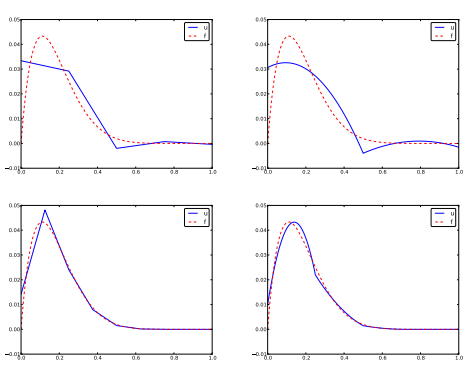
\includegraphics[width=0.7\linewidth]{img_29}
	\caption{Comparison of the finite element approximations: 4 P1 elements with
		5 nodes (upper left), 2 P2 elements with 5 nodes (upper right), 8 P1 elements
		with 9 nodes (lower left), and 4 P2 elements with 9 nodes (lower right).}
	\label{fig:img_29}
\end{figure}
\section[Sparse matrix storage and solution]{Sparse matrix storage and solution}
\label{sec:sec_4_8}
\noindent Some of the examples in the preceding section took several minutes to compute, even on small meshes consisting of up to eight elements. The main explanation for slow computations is unsuccessful symbolic integration: sympy may use a lot of energy on integrals like $\int f(x(X)) \tilde{\varphi}_{r}(X) h / 2 d x$ before giving up, and the program then resorts to numerical integration. Codes that can deal with a large number of basis functions and accept flexible choices of $f(x)$ should compute all integrals numerically and replace the matrix objects from sympy by the far more efficient array objects from numpy.

Another reason for slow code is related to the fact that most of the matrix entries $A_{i, j}$ are zero, because $\left(\varphi_{i}, \varphi_{j}\right)=0$ unless $i$ and $j$ are nodes in the same element. A matrix whose majority of entries are zeros, is known as a sparse matrix. The sparsity should be utilized in software as it dramatically decreases the storage demands and the CPU-time needed to compute the solution of the linear system. This optimization is not critical in 1D problems where modern computers can afford computing with all the zeros in the complete square matrix, but in $2 \mathrm{D}$ and especially in 3D, sparse matrices are fundamental for feasible finite element computations.

In 1D problems, using a numbering of nodes and elements from left to right
over the domain, the assembled coefficient matrix has only a few diagonals
different from zero. More precisely, 2d + 1 diagonals are different from zero.
With a different numbering of global nodes, say a random ordering, the diagonal
structure is lost, but the number of nonzero elements is unaltered. Figures \hyperref[fig:img_30]{30}
and \hyperref[fig:img_31]{31} exemplify sparsity patterns.
\begin{figure}[H]
	\centering
	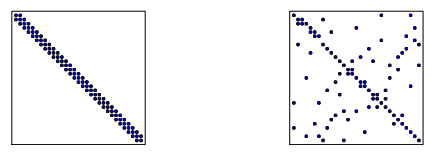
\includegraphics[width=0.7\linewidth]{img_30}
	\caption{Matrix sparsity pattern for left-to-right numbering (left) and random
		numbering (right) of nodes in P1 elements.}
	\label{fig:img_30}
\end{figure}
\begin{figure}[H]
	\centering
	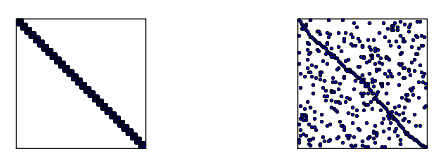
\includegraphics[width=0.7\linewidth]{img_31}
	\caption{Matrix sparsity pattern for left-to-right numbering (left) and random
		numbering (right) of nodes in P3 elements.}
	\label{fig:img_31}
\end{figure}

The scipy.sparse library supports creation of sparse matrices and linear system solution.
\begin{itemize}
	\item scipy.sparse.diags for matrix defined via diagonals
	\item scipy.sparse.lil\textunderscore matrix for creation via setting matrix entries
	\item scipy.sparse.dok\textunderscore matrix for creation via setting matrix entries
\end{itemize}
\chapter{Comparison of finite element and finite difference approximation}
\label{chap:chap_5}
\noindent The previous sections on approximating f by a finite element function u utilize
the projection/Galerkin or least squares approaches to minimize the approximation error. We may, alternatively, use the collocation/interpolation method
as described in Section \hyperref[sec:sec_4_4]{4.4}. Here we shall compare these three approaches with
what one does in the finite difference method when representing a given function
on a mesh.
\section[Finite difference approximation of given functions]{Finite difference approximation of given functions}
\label{sec:sec_5_1}
Approximating a given function $f(x)$ on a mesh in a finite difference context will typically just sample $f$ at the mesh points. If $u_{\imath}$ is the value of the approximate $u$ at the mesh point $x_{i}$, we have $u_{i}=f\left(x_{i}\right)$. The collocation/interpolation method using finite element basis functions gives exactly the same representation, as shown Section \hyperref[sec:sec_4_4]{4.4},
$$
u\left(x_{i}\right)=c_{i}=f\left(x_{i}\right) .
$$
How does a finite element Galerkin or least squares approximation differ from this straightforward interpolation of $f$ ? This is the question to be addressed next. We now limit the scope to $\mathrm{P} 1$ elements since this is the element type that gives formulas closest to those arising in the finite difference method.
\section[Finite difference interpretation of a finite element approximation]{Finite difference interpretation of a finite element approximation}
\label{sec:sec_5_2}
The linear system arising from a Galerkin or least squares approximation reads in general
$$
\sum_{j \in \mathcal{I}_{s}} c_{j}\left(\psi_{i}, \psi_{j}\right)=\left(f, \psi_{i}\right), \quad i \in \mathcal{I}_{s}.
$$
In the finite element approximation we choose $\psi_{i}=\varphi_{i}$. With $\varphi_{i}$ corresponding to $\mathrm{P} 1$ elements and a uniform mesh of element length $h$ we have in Section \hyperref[sec:sec_3_6]{3.6} calculated the matrix with entries $\left(\varphi_{i}, \varphi_{j}\right)$. Equation number $i$ reads
\begin{equation}\label{eqa84}
	\frac{h}{6}\left(u_{i-1}+4 u_{i}+u_{i+1}\right)=\left(f, \varphi_{i}\right).
\end{equation}
The first and last equation, corresponding to $i=0$ and $i=N$ are slightly different, see Section \hyperref[sec:sec_4_6]{4.6}.

The finite difference counterpart to (\hyperref[eqa84]{84}) is just $u_{i}=f_{i}$ as explained in Section \hyperref[sec:sec_5_1]{5.1}. To easier compare this result to the finite element approach to approximating functions, we can rewrite the left-hand side of (\hyperref[eqa84]{84}) as
\begin{equation}\label{eqa85}
	h\left(u_{i}+\frac{1}{6}\left(u_{i-1}-2 u_{i}+u_{i+1}\right)\right).
\end{equation}
Thinking in terms of finite differences, we can write this expression using finite difference operator notation:
$$
\left[h\left(u+\frac{h^{2}}{6} D_{x} D_{x} u\right)\right]_{i},
$$
which is nothing but the standard discretization of
$$
h\left(u+\frac{h^{2}}{6} u^{\prime \prime}\right) .
$$
Before interpreting the approximation procedure as solving a differential equation, we need to work out what the right-hand side is in the context of P1 elements. Since $\varphi_{i}$ is the linear function that is 1 at $x_{i}$ and zero at all other nodes, only the interval $\left[x_{i-1}, x_{i+1}\right]$ contribute to the integral on the right-hand side. This integral is naturally split into two parts according to (\hyperref[eqa54]{54}):
$$
\left(f, \varphi_{i}\right)=\int_{x_{i-1}}^{x_{i}} f(x) \frac{1}{h}\left(x-x_{i-1}\right) d x+\int_{x_{i}}^{x_{i+1}} f(x) \frac{1}{h}\left(1-\left(x-x_{i}\right)\right) d x.
$$
However, if $f$ is not known we cannot do much else with this expression. It is clear that many values of $f$ around $x_{i}$ contributes to the right-hand side, not just the single point value $f\left(x_{i}\right)$ as in the finite difference method.

To proceed with the right-hand side, we can turn to numerical integration schemes. The Trapezoidal method for $\left(f, \varphi_{i}\right)$, based on sampling the integrand $f \varphi_{i}$ at the node points $x_{i}=i h$ gives
$$
\left(f, \varphi_{i}\right)=\int_{\Omega} f \varphi_{i} d x \approx h \frac{1}{2}\left(f\left(x_{0}\right) \varphi_{i}\left(x_{0}\right)+f\left(x_{N}\right) \varphi_{i}\left(x_{N}\right)\right)+h \sum_{j=1}^{N-1} f\left(x_{j}\right) \varphi_{i}\left(x_{j}\right) .
$$
Since $\varphi_{i}$ is zero at all these points, except at $x_{i}$, the Trapezoidal rule collapses to one term:
\begin{equation}\label{eqa86}
	\left(f, \varphi_{i}\right) \approx h f\left(x_{i}\right),
\end{equation}
for $i=1, \ldots, N-1$, which is the same result as with collocation/interpolation, and of course the same result as in the finite difference method. For $i=0$ and $i=N$ we get contribution from only one element so
\begin{equation}\label{eqa87}
	\left(f, \varphi_{i}\right) \approx \frac{1}{2} h f\left(x_{i}\right), \quad i=0, i=N .
\end{equation}
Simpson's rule with sample points also in the middle of the elements, at $x_{i+\frac{1}{2}}=\left(x_{i}+x_{i+1}\right) / 2$, can be written as
$$
\int_{\Omega} g(x) d x \approx \frac{\tilde{h}}{3}\left(g\left(x_{0}\right)+2 \sum_{j=1}^{N-1} g\left(x_{j}\right)+4 \sum_{j=0}^{N-1} g\left(x_{j+\frac{1}{2}}\right)+f\left(x_{2 N}\right)\right),
$$
where $\tilde{h}=h / 2$ is the spacing between the sample points. Our integrand is $g=$ $f \varphi_{i}$. For all the node points, $\varphi_{i}\left(x_{j}\right)=\delta_{i j}$, and therefore $\sum_{j=1}^{N-1} f\left(x_{j}\right) \varphi_{i}\left(x_{j}\right)=$ $f\left(x_{i}\right)$. At the midpoints, $\varphi_{i}\left(x_{i \pm \frac{1}{2}}\right)=1 / 2$ and $\varphi_{i}\left(x_{j+\frac{1}{2}}\right)=0$ for $j>1$ and $j<i-1$. Consequently,
$$
\sum_{j=0}^{N-1} f\left(x_{j+\frac{1}{2}}\right) \varphi_{i}\left(x_{j+\frac{1}{2}}\right)=\frac{1}{2}\left(f x_{j-\frac{1}{2}}+x_{j+\frac{1}{2}}\right) \text {. }
$$
When $1 \leq i \leq N-1$ we then get
\begin{equation}\label{eqa88}
	\left(f, \varphi_{i}\right) \approx \frac{h}{3}\left(f_{i-\frac{1}{2}}+f_{i}+f_{i+\frac{1}{2}}\right) .
\end{equation}
This result shows that, with Simpson's rule, the finite element method operates with the average of $f$ over three points, while the finite difference method just applies $f$ at one point. We may interpret this as a "smearing" or smoothing of $f$ by the finite element method.

We can now summarize our findings. With the approximation of $\left(f, \varphi_{i}\right)$ by the Trapezoidal rule, P1 elements give rise to equations that can be expressed as a finite difference discretization of
\begin{equation}\label{eqa89}
	u+\frac{h^{2}}{6} u^{\prime \prime}=f, \quad u^{\prime}(0)=u^{\prime}(L)=0,
\end{equation}
expressed with operator notation as
\begin{equation}\label{eqa90}
	\left[u+\frac{h^{2}}{6} D_{x} D_{x} u=f\right]_{i}.
\end{equation}
As $h \rightarrow 0$, the extra term proportional to $u^{\prime \prime}$ goes to zero, and the two methods are then equal.
With the Simpson's rule, we may say that we solve
\begin{equation}\label{eqa91}
	\left[u+\frac{h^{2}}{6} D_{x} D_{x} u=\bar{f}\right]_{i},
\end{equation}
where $\bar{f}_{i}$ means the average $\frac{1}{3}\left(f_{i-1 / 2}+f_{i}+f_{i+1 / 2}\right)$.

The extra term $\frac{h^{2}}{6} u^{\prime \prime}$ represents a smoothing effect: with just this term, we would find $u$ by integrating $f$ twice and thereby smooth $f$ considerably. In addition, the finite element representation of $f$ involves an average, or a smoothing, of $f$ on the right-hand side of the equation system. If $f$ is a noisy function, direct interpolation $u_{i}=f_{i}$ may result in a noisy $u$ too, but with a Galerkin or least squares formulation and P1 elements, we should expect that $u$ is smoother than $f$ unless $h$ is very small.

The interpretation that finite elements tend to smooth the solution is valid in applications far beyond approximation of $1 \mathrm{D}$ functions.

\section[Making finite elements behave as finite differences]{Making finite elements behave as finite differences}
\label{sec:sec_5_3}
\noindent With a simple trick, using numerical integration, we can easily produce the result $u_{i}=f_{i}$ with the Galerkin or least square formulation with P1 elements. This is useful in many occasions when we deal with more difficult differential equations and want the finite element method to have properties like the finite difference method (solving standard linear wave equations is one primary example).

\noindent \textbf{Computations in physical space.} We have already seen that applying the Trapezoidal rule to the right-hand side $\left(f, \varphi_{i}\right)$ simply gives $f$ sampled at $x_{i}$. Using the Trapezoidal rule on the matrix entries $A_{i, j}=\left(\varphi_{i}, \varphi_{j}\right)$ involves a sum
$$
\sum_{k} \varphi_{i}\left(x_{k}\right) \varphi_{j}\left(x_{k}\right),
$$
but $\varphi_{i}\left(x_{k}\right)=\delta_{i k}$ and $\varphi_{j}\left(x_{k}\right)=\delta_{j k}$. The product $\varphi_{i} \varphi_{j}$ is then different from zero only when sampled at $x_{i}$ and $i=j$. The Trapezoidal approximation to the integral is then
$$
\left(\varphi_{i}, \varphi_{j}\right) \approx h, \quad i=j,
$$
and zero if $i \neq j$. This means that we have obtained a diagonal matrix! The first and last diagonal elements, $\left(\varphi_{0}, \varphi_{0}\right)$ and $\left(\varphi_{N}, \varphi_{N}\right)$ get contribution only from the first and last element, respectively, resulting in the approximate integral value $h / 2$. The corresponding right-hand side also has a factor $1 / 2$ for $i=0$ and $i=N$. Therefore, the least squares or Galerkin approach with $\mathrm{P} 1$ elements and Trapezoidal integration results in
$$
c_{i}=f_{i}, \quad i \in \mathcal{I}_{s} .
$$
Simpsons's rule can be used to achieve a similar result for $\mathrm{P} 2$ elements, i.e, a diagonal coefficient matrix, but with the previously derived average of $f$ on the right-hand side.
\bigbreak
\noindent \textbf{Elementwise computations.} Identical results to those above will arise if we perform elementwise computations. The idea is to use the Trapezoidal rule on the reference element for computing the element matrix and vector. When assembled, the same equations $c_{i}=f\left(x_{i}\right)$ arise. Exercise \hyperref[sec:sec_10_19]{19} encourages you to carry out the details.
\bigbreak
\noindent \textbf{Terminology}. The matrix with entries $\left(\varphi_{i}, \varphi_{j}\right)$ typically arises from terms proportional to $u$ in a differential equation where $u$ is the unknown function. This matrix is often called the mass matrix, hecause in the early days of the finite element method, the matrix arose from the mass times acceleration term in Newton's second law of motion. Making the mass matrix diagonal by, e.g., numerical integration, as demonstrated above, is a widely used technique and is called mass lumping. In time-dependent problems it can sometimes enhance the numerical accuracy and computational efficiency of the finite element method. However, there are also examples where mass lumping destroys accuracy.

\chapter{A generalized element concept}
\label{chap:chap_6}
\noindent So far, finite element computing has employed the nodes and element lists
together with the definition of the basis functions in the reference element.

Suppose we want to introduce a piecewise constant approximation with one basis function $\tilde{\varphi}_{0}(x)=1$ in the reference element, corresponding to a $\varphi_{i}(x)$ function that is 1 on element number $i$ and zero on all other elements. Although we could associate the function value with a node in the middle of the elements, there are no nodes at the ends, and the previous code snippets will not work because we cannot find the element boundaries from the nodes list.
\section[Cells, vertices, and degrees of freedom]{Cells, vertices, and degrees of freedom}
\label{sec:sec_6_1}
We now introduce \textit{cells} as the subdomains $\Omega^{(e)}$ previously referred as elements. The cell boundaries are denoted as \textit{vertices}. The reason for this name is that cells are recognized by their vertices in $2 \mathrm{D}$ and 3D. We also define a \textit{set of degrees of freedom}, which are the quantities we aim to compute. The most common type of degree of freedom is the value of the unknown function $u$ at some point. (For example, we can introduce nodes as before and say the degrees of freedom are the values of $u$ at the nodes.) The basis functions are constructed so that they equal unity for one particular degree of freedom and zero for the rest. This property ensures that when we evaluate $u=\sum_{j} c_{j} \varphi_{j}$ for degree of freedom number $i$, we get $u=c_{i}$. Integrals are performed over cells, usually by mapping the cell of interest to a \textit{reference cell}.

With the concepts of cells, vertices, and degrees of freedom we increase the decoupling of the geometry (cell, vertices) from the space of basis functions. We will associate different sets of basis functions with a cell. In 1D, all cells are intervals, while in 2D we can have cells that are triangles with straight sides, or any polygon, or in fact any two-dimensional geometry. Triangles and quadrilaterals are most common, though. The popular cell types in $3 \mathrm{D}$ are tetrahedra and hexahedra.
\section[Extended finite element concept]{Extended finite element concept}
\label{sec:sec_6_2}
The concept of a finite element is now
\begin{itemize}
	\item a \textit{reference cell} in a local reference coordinate system;
	\item a set of \textit{basis functions} $\tilde{\varphi}_{i}$ defined on the cell;
	\item a set of \textit{degrees of freedom} that uniquely determines the basis functions such that $\tilde{\rho}_{i}=1$ for degree of freedom number $i$ and $\tilde{\rho}_{i}=0$ for all other degrees of freedom;
	\item a mapping between local and global degree of freedom numbers, here called the \textit{dof map};
	\item a geometric \textit{mapping} of the reference cell onto to cell in the physical domain.
\end{itemize}
There must be a geometric description of a cell. This is trivial in 1D since the
cell is an interval and is described by the interval limits, here called vertices. If the cell is $\Omega^{(e)}=\left[x_{L}, x_{R}\right]$, vertex 0 is $x_{L}$ and vertex 1 is $x_{R}$. The reference cell in $1 \mathrm{D}$ is $[-1,1]$ in the reference coordinate system $X$.
The expansion of $u$ over one cell is often used:
\begin{equation}\label{eqa92}
	u(x)=\tilde{u}(X)=\sum_{r} c_{r} \tilde{\rho}_{r}(X), \quad x \in \Omega^{(e)}, X \in[-1,1],
\end{equation}
where the sum is taken over the numbers of the degrees of freedom and $c_{r}$ is the value of $u$ for degree of freedom number $r$.

Our previous $\mathrm{P} 1, \mathrm{P} 2$, etc., elements are defined by introducing $d+1$ equally spaced nodes in the reference cell and saying that the degrees of freedom are the $d+1$ function values at these nodes. The basis functions must be 1 at one node and 0 at the others, and the Lagrange polynomials have exactly this property. The nodes can be numbered from left to right with associated degrees of freedom that are numbered in the same way. The degree of freedom mapping becomes what was previously represented by the elements lists. The cell mapping is the same affine mapping (\hyperref[eqa61]{61}) as before.
\section[Implementation]{Implementation}
\label{sec:sec_6_3}
\noindent Implementationwise,
\begin{itemize}
	\item we replace nodes by vertices;
	\item we introduce cells such that cell [e] [r] gives the mapping from local vertex $r$ in cell e to the global vertex number in vertices;
	\item we replace elements by dof\textunderscore map (the contents are the same for $\mathrm{P} d$ elements).
\end{itemize}

\noindent Consider the example from Section \hyperref[sec:sec_3_1]{3.1} where $\Omega=[0,1]$ is divided into two cells, $\Omega^{(0)}=[0,0.4]$ and $\Omega^{(1)}=[0.4,1]$, as depicted in Figure \hyperref[fig:img_16]{16} . The vertices are $[0,0.4,1]$. Local vertex 0 and 1 are 0 and $0.4$ in cell 0 and $0.4$ and 1 in cell 1 . A P2 element means that the degrees of freedom are the value of $u$ at three equally spacèd points (nodes) in each céll. The data structuress become
\begin{lstlisting}[numbers=none]
vertices = [0, 0.4, 1]
cells = [[0, 1], [1, 2]]
dof_map = [[0, 1, 2], [2, 3, 4]]	
\end{lstlisting}
If we would approximate $f$ by piecewise constants, known as $\mathrm{P} 0$ elements, we simply introduce one point or node in an element, preferably $X=0$, and define one degree of freedom, which is the function value at this node. Moreover, we set $\tilde{\varphi}_{0}(X)=1$. The cells and vertices arrays remain the same, but dof\textunderscore map is altered:
\begin{lstlisting}[numbers=none]
dof_map = [[0], [1]]	
\end{lstlisting}
We use the cells and vertices lists to retrieve information on the geometry of a cell, while dof\textunderscore map is the $q(e, r)$ mapping introduced earlier in the assembly of element matrices and vectors. For example, the Omega\textunderscore e variable (representing the cell interval) in previous code snippets must now be computed as
\begin{lstlisting}[numbers=none]
Omega_e = [vertices[cells[e][0], vertices[cells[e][1]]	
\end{lstlisting}
The assembly is done by
\begin{lstlisting}[numbers=none]
A[dof_map[e][r], dof_map[e][s]] += A_e[r,s]
b[dof_map[e][r]] += b_e[r]	
\end{lstlisting}
We will hereafter drop the nodes and elements arrays and work exculsively
with cells, vertices, and dof\textunderscore map. The module fe\textunderscore approx1D\textunderscore numint.py
now replaces the module fe\textunderscore approx1D and offers similar functions that work
with the new concepts:
\begin{lstlisting}[numbers=none]
from fe_approx1D_numint import *
x = sp.Symbol('x')
f = x*(1 - x)
N_e = 10
vertices, cells, dof_map = mesh_uniform(N_e, d=3, Omega=[0,1])
phi = [basis(len(dof_map[e])-1) for e in range(N_e)]
A, b = assemble(vertices, cells, dof_map, phi, f)
c = np.linalg.solve(A, b)
# Make very fine mesh and sample u(x) on this mesh for plotting
x_u, u = u_glob(c, vertices, cells, dof_map,
				resolution_per_element=51)
plot(x_u, u)	
\end{lstlisting}
These steps are offered in the approximate function, which we here apply to see
how well four P0 elements (piecewise constants) can approximate a parabola:
\begin{lstlisting}[numbers=none]
from fe_approx1D_numint import *
x=sp.Symbol("x")
for N_e in 4, 8:
	approximate(x*(1-x), d=0, N_e=N_e, Omega=[0,1])	
\end{lstlisting}
Figure \hyperref[fig:img_32]{32} shows the result.

\section[Computing the error of the approximation]{Computing the error of the approximation}
\label{sec:sec_6_4}
So far we have focused on computing the coefficients $c_{j}$ in the approximation $u(x)=\sum_{j} c_{j} \varphi_{j}$ as well as on plotting $u$ and $f$ for visual comparison. A more quantitative comparison needs to investigate the error $e(x)=f(x)-u(x)$. We mostly want a single number to reflect the error and use a norm for this purpose, usually the $L^{2}$ norm
$$
\|e\|_{L^{2}}=\left(\int_{\Omega} e^{2} d x\right)^{1 / 2}.
$$
\begin{figure}[H]
	\centering
	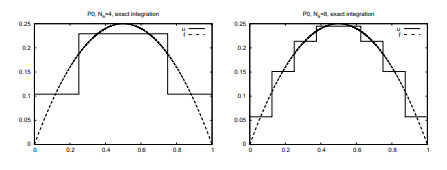
\includegraphics[width=0.7\linewidth]{img_32}
	\caption{Approximation of a parabola by 4 (left) and 8 (right) P0 elements.}
	\label{fig:img_32}
\end{figure}
\noindent Since the finite element approximation is defined for all $x \in \Omega$, and we are interested in how $u(x)$ deviates from $f(x)$ through all the elements, we can either integrate analytically or use an accurate numerical approximation. The latter is more convenient as it is a generally feasible and simple approach. The idea is to sample $e(x)$ at a large number of points in each element. The function u\textunderscore glob in the fe\textunderscore approx1D\textunderscore numint module does this for $u(x)$ and returns an array $\mathbf{x}$ with coordinates and an array $u$ with the $u$ values:
\begin{lstlisting}[numbers=none]
x, u = u_glob(c, vertices, cells, dof_map,
			resolution_per_element=101)
e = f(x) - u
\end{lstlisting}
Let us use the Trapezoidal method to approximate the integral. Because different
elements may have different lengths, the x array has a non-uniformly distributed
set of coordinates. Also, the u\textunderscore glob function works in an element by element
fashion such that coordinates at the boundaries between elements appear twice.
We therefore need to use a ”raw” version of the Trapezoidal rule where we just
add up all the trapezoids:
$$
\int_{\Omega} g(x) d x \approx \sum_{j=0}^{n-1} \frac{1}{2}\left(g\left(x_{j}\right)+g\left(x_{j+1}\right)\right)\left(x_{j+1}-x_{j}\right),
$$
if $x_{0}, \ldots, x_{n}$ are all the coordinates in $\mathrm{x}$. In vectorized Python code,
\begin{lstlisting}[numbers=none]
g_x = g(x)
integral = 0.5*np.sum((g_x[:-1] + g_x[1:])*(x[1:] - x[:-1]))	
\end{lstlisting}
Computing the $L^{2}$ norm of the error, here named E, is now achieved by
\begin{lstlisting}[numbers=none]
e2 = e**2
E = np.sqrt(0.5*np.sum((e2[:-1] + e2[1:])*(x[1:] - x[:-1]))	
\end{lstlisting}
\begin{mybox}
	\textbf{How does the error depend on $h$ and $d$ ?}
	
	\noindent Theory and experiments show that the least squares or projection/Galerkin method in combination with $\mathrm{P} d$ elements of equal length $h$ has an error
	\begin{equation}\label{eqa93}
		\|e\|_{L^{2}}=C h^{d+1},
	\end{equation}
	
	\noindent where $C$ is a constant depending on $f$, but not on $h$ or $d$.
\end{mybox}

\section[Example: Cubic Hermite polynomials]{Example: Cubic Hermite polynomials}
\label{sec:sec_6_5}
The finite elements considered so far represent u as piecewise polynomials with
discontinuous derivatives at the cell boundaries. Sometimes it is desirable to
have continuous derivatives. A primary examples is the solution of differential
equations with fourth-order derivatives where standard finite element formulations lead to a need for basis functions with continuous first-order derivatives.
The most common type of such basis functions in 1D is the so-called cubic
Hermite polynomials. The construction of such polynomials, as explained next,
will further exemplify the concepts of a cell, vertex, degree of freedom, and dof
map.

Given a reference cell $[-1,1]$, we seek cubic polynomials with the values of the \textit{function} and its \textit{first-order derivative} at $X=-1$ and $X=1$ as the four degrees of freedom. Let us number the degrees of freedom as
\begin{itemize}
	\item 0 : value of function at $X=-1$
	\item 1: value of first derivative at $X=-1$
	\item 2: value of function at $X=1$
	\item 3: value of first derivative at $X=1$
\end{itemize}
By having the derivatives as unknowns, we ensure that the derivative of a basis function in two neighboring elements is the same at the node points.
The four basis functions can be written in a general form
$$
\tilde{\varphi}_{i}(X)=\sum_{j=0}^{3} C_{i, j} X^{j},
$$
with four coefficients $C_{i, j}, j=0,1,2,3$, to be determined for each $i$. The constraints that basis function number $i$ must be 1 for degree of freedom number $i$ and zero for the other three degrees of freedom, gives four equations to determine $C_{i, j}$ for each $i$. In mathematical detail,
$$
\begin{aligned}
	\tilde{\varphi}_{0}(-1)=1, & \tilde{\varphi}_{0}(1)=\tilde{\varphi}_{0}^{\prime}(-1)=\tilde{\varphi}_{i}^{\prime}(1)=0, \\
	\tilde{\varphi}_{1}^{\prime}(-1)=1, & \tilde{\varphi}_{1}(-1)=\tilde{\varphi}_{1}(1)=\tilde{\varphi}_{1}^{\prime}(1)=0, \\
	\tilde{\varphi}_{2}(1)=1, & \tilde{\varphi}_{2}(-1)=\tilde{\varphi}_{2}^{\prime}(-1)=\tilde{\varphi}_{2}^{\prime}(1)=0, \\
	\tilde{\varphi}_{3}^{\prime}(1)=1, & \tilde{\varphi}_{3}(-1)=\tilde{\varphi}_{3}^{\prime}(-1)=\tilde{\varphi}_{3}(1)=0 .
\end{aligned}
$$
These four $4 \times 4$ linear equations can be solved, yielding the following formulas for the cubic basis functions:
\begin{equation}\label{eqa94}
	\tilde{\varphi}_{0}(X) =1-\frac{3}{4}(X+1)^{2}+\frac{1}{4}(X+1)^{3}
\end{equation}
\begin{equation}\label{eqa95}
	\tilde{\varphi}_{1}(X) =-(X+1)\left(1-\frac{1}{2}(X+1)\right)^{2}
\end{equation}
\begin{equation}\label{eqa96}
	\tilde{\varphi}_{2}(X) =\frac{3}{4}(X+1)^{2}-\frac{1}{2}(X+1)^{3}
\end{equation}
\begin{equation}\label{eqa97}
	\tilde{\varphi}_{3}(X) =-\frac{1}{2}(X+1)\left(\frac{1}{2}(X+1)^{2}-(X+1)\right)
\end{equation}
\begin{equation}\label{eqa98}
\end{equation}	
The construction of the dof map needs a scheme for numbering the global degrees of freedom. A natural left-to-right numbering has the function value at vertex $x_{i}$ as degree of freedom number $2 i$ and the value of the derivative at $x_{i}$ as degree of freedom number $2 i+1, i=0, \ldots, N_{e}+1$.
\chapter{Numerical integration}
\label{chap:chap_7}
\noindent Finite element codes usually apply numerical approximations to integrals. Since the integrands in the coefficient matrix often are (lower-order) polynomials, integration rules that can integrate polynomials cxactly are popular.
The numerical integration rules can be expressed in a common form,
\begin{equation}\label{eqa99}
	\int_{-1}^{1} g(X) d X \approx \sum_{j=0}^{M} w_{j} g\left(\bar{X}_{j}\right),
\end{equation}	
where $\bar{X}_{j}$ are integration points and $w_{j}$ are integration weights, $j=0, \ldots, M$. Different rules correspond to different choices of points and weights.
The very simplest method is the Midpoint rule,
\begin{equation}\label{eqa100}
	\int_{-1}^{1} g(X) d X \approx 2 g(0), \quad \bar{X}_{0}=0, w_{0}=2,
\end{equation}	
which integrates linear functions exactly.
\section[Newton-Cotes rules]{Newton-Cotes rules}
\label{sec:sec_7_1}
\noindent The \href{https://en.wikipedia.org/wiki/Newton%E2%80%93Cotes_formulas}{Newton-Cotes} rules are based on a fixed uniform distribution of the integration points. The first two formulas in this family are the well-known \textit{Trapezoidal rule},
\begin{equation}\label{eqa101}
	\int_{-1}^{1} g(X) d X \approx g(-1)+g(1), \quad \bar{X}_{0}=-1, \quad \bar{X}_{1}=1, w_{0}=w_{1}=1,
\end{equation}
and \textit{Simpson's rule},
\begin{equation}\label{eqa102}
	\int_{-1}^{1} g(X) d X \approx \frac{1}{3}(g(-1)+4 g(0)+g(1)),
\end{equation}
where
\begin{equation}\label{eqa103}
	\bar{X}_{0}=-1, \bar{X}_{1}=0, \bar{X}_{2}=1, w_{0}=w_{2}=\frac{1}{3}, w_{1}=\frac{4}{3}.
\end{equation}
Newton-Cotes rules up to five points is supported in the module file \href{https://github.com/hplgit/INF5620/blob/master/src/fem/numint.py}{numint.py.}

For higher accuracy one can divide the reference cell into a set of subintervals and use the rules above on each subinterval. This approach results in composite rules, well-known from basic introductions to numerical integration of $\int_{a}^{b} f(x) d x$.
\bigbreak
\section[Gauss-Legendre rules with optimized points]{Gauss-Legendre rules with optimized points}
\label{sec:sec_7_2}
More accurate rules, for a given $M$, arise if the location of the integration points are optimized for polynomial integrands. The\href{https://en.wikipedia.org/wiki/Gaussian_quadrature}{Gauss-Legendre rules} (also known as Gauss-Legendre quadrature or Gaussian quadrature) constitute one such class of integration methods. Two widely applied Gauss-Legendre rules in this family have the choice
\begin{equation}\label{eqa104}
	M=1: \bar{X}_{0}=-\frac{1}{\sqrt{3}}, \bar{X}_{1}=\frac{1}{\sqrt{3}}, w_{0}=w_{1}=1
\end{equation}
\begin{equation}\label{eqa105}
	M=2: \bar{X}_{0}=-\sqrt{\frac{3}{5}}, \bar{X}_{0}=0, \bar{X}_{2}=\sqrt{\frac{3}{5}}, w_{0}=w_{2}=\frac{5}{9}, w_{1}=\frac{8}{9}.
\end{equation}
These rules integrate 3 rd and 5 th degree polynomials exactly. In general, an $M$-point Gauss-Legendre rule integrates a polynomial of degree $2 M+1$ exactly. The code numint.py contains a large collection of Gauss-Legendre rules.
\chapter{Approximation of functions in 2D}
\label{chap:chap_8}
\noindent All the concepts and algorithms developed for approximation of $1 \mathrm{D}$ functions $f(x)$ can readily be extended to $2 \mathrm{D}$ functions $f(x, y)$ and $3 \mathrm{D}$ functions $f(x, y, z)$. Basically, the extensions consists of defining basis functions $\psi_{i}(x, y)$ or $\psi_{i}(x, y, z)$ over some domain $\Omega$, and for the least squares and Galerkin methods, the integration is done over $\Omega$.

As in 1D, the least squares and projection/Galerkin methods two lead to linear systems
$$
\begin{aligned}
	\sum_{j \in \mathcal{I}_{s}} A_{i, j} c_{j} &=b_{i}, \quad i \in \mathcal{I}_{s}, \\
	A_{i, j} &=\left(\psi_{i}, \psi_{j}\right), \\
	b_{i} &=\left(f, \psi_{i}\right),
\end{aligned}
$$
where the inner product of two functions $f(x, y)$ and $g(x, y)$ is defined completely analogously to the $1 \mathrm{D}$ case (\hyperref[eqa24]{24}) :
\begin{equation}\label{eqa106}
	(f, g)=\int_{\Omega} f(x, y) g(x, y) d x d y
\end{equation}
\section[2D basis functions as tensor products of 1D functions]{2D basis functions as tensor products of 1D functions}
\label{sec:sec_8_1}

\noindent One straightforward way to construct a basis in $2 \mathrm{D}$ is to combine $1 \mathrm{D}$ basis functions. Say we have the $1 \mathrm{D}$ vector space
\begin{equation}\label{eqa107}
	V_{x}=\operatorname{span}\left\{\hat{\psi}_{0}(x), \ldots, \hat{\psi}_{N_{x}}(x)\right\}.
\end{equation}
A similar space for variation in $y$ can be defined,
\begin{equation}\label{eqa108}
	V_{y}=\operatorname{span}\left\{\hat{\psi}_{0}(y), \ldots, \hat{\psi}_{N_{y}}(y)\right\}.
\end{equation}
We can then form 2D basis functions as tensor products of 1D basis functions.
\begin{mybox}
	\textbf{Tensor products.}
	
	Given two vectors $a=\left(a_{0}, \ldots, a_{M}\right)$ and $b=\left(b_{0}, \ldots, b_{N}\right)$, their outer tensor product, also called the dyadic product, is $p=a \otimes b$, defined through
	$$
	p_{i, j}=a_{i} b_{j}, \quad i=0, \ldots, M, j=0, \ldots, N .
	$$
	In the tensor terminology, $a$ and $b$ are first-order tensors (vectors with one
	index, also termed rank-1 tensors). The corresponding \textit{inner tensor product} is the well-known scalar or dot product of two vectors: $p=a \cdot b=\sum_{j=0}^{N} a_{j} b_{j}$. Now, $p$ is a rank-0 tensor.
	
	Tensors are typically represented by arrays in computer code. In the above example, $a$ and $b$ are represented by one-dimensional arrays of length $M$ and $N$, respectively, while $p=a \otimes b$ must be represented by a twodimensional array of size $M \times N$.
	
	\href{https://en.wikipedia.org/wiki/Tensor_product}{Tensor products} can be used in a variety of context.
\end{mybox}

Given the vector spaces $V_{x}$ and $V_{y}$ as defined in (107) and (108), the tensor product space $V=V_{x} \otimes V_{y}$ has a basis formed as the tensor product of the basis for $V_{x}$ and $V_{y}$. That is, if $\left\{\varphi_{i}(x)\right\}_{i \in \mathcal{I}_{x}}$ and $\left\{\varphi_{i}(y)\right\}_{i \in \mathcal{I}_{y}}$ are basis for $V_{x}$ and $V_{y}$, respectively, the elements in the basis for $V$ arise from the tensor product: $\left\{\varphi_{i}(x) \varphi_{j}(y)\right\}_{i \in \mathcal{I}_{x}, j \in \mathcal{I}_{y}}$. The index sets are $I_{x}=\left\{0, \ldots, N_{x}\right\}$ and $I_{y}=\left\{0, \ldots, N_{y}\right\}$.

The notation for a basis function in 2D can employ a double index as in
$$
\psi_{p, q}(x, y)=\hat{\psi}_{p}(x) \hat{\psi}_{q}(y), \quad p \in \mathcal{I}_{x}, q \in \mathcal{I}_{y}.
$$

The expansion for u is then written as a double sum

$$
u=\sum_{p \in \mathcal{I}_{x}} \sum_{q \in \mathcal{I}_{y}} c_{p, q} \psi_{p, q}(x, y).
$$
Alternatively, we may employ a single index,
$$
\psi_{i}(x, y)=\hat{\psi}_{p}(x) \hat{\psi}_{q}(y),
$$
and use the standard form for $u$,
$$
u=\sum_{j \in \mathcal{I}_{s}} c_{j} \psi_{j}(x, y).
$$
The single index is related to the double index through $i=p N_{y}+q$ or $i=q N_{x}+p$.
\bigbreak

\section[Example: Polynomial basis in 2D]{Example: Polynomial basis in 2D}
\label{sec:sec_8_2}
\noindent Suppose we choose $\hat{\psi}_{p}(x)=x^{p}$, and try an approximation with $N_{x}=N_{y}=1$ :
$$
\psi_{0,0}=1, \quad \psi_{1,0}=x, \quad \psi_{0,1}=y, \quad \psi_{1,1}=x y.
$$
Using a mapping to one index like $i=q N_{x}+p$, we get
$$
\psi_{0}=1, \quad \psi_{1}=x, \quad \psi_{2}=y, \quad \psi_{3}=x y.
$$
With the specific choice $f(x, y)=\left(1+x^{2}\right)\left(1+2 y^{2}\right)$ on $\Omega=\left[0, L_{x}\right] \times\left[0, L_{y}\right]$, we can perform actual calculations:
$$
\begin{aligned}
	&A_{u, 0}=\left(\psi_{0}, \psi_{0}\right)=\int_{0}^{L_{y}} \int_{0}^{L_{x}} \psi_{0}(x, y)^{2} d x d y=\int_{0}^{L_{y}} \int_{0}^{L_{x}} d x d y=L_{x} L_{y}, \\
	&A_{1,0}=\left(\psi_{1}, \psi_{0}\right)=\int_{0}^{L_{y}} \int_{0}^{L_{x}} x d x d y=\frac{1}{2} L_{x}^{2} L_{y}, \\
	&A_{0,1}=\left(\psi_{0}, \psi_{1}\right)=\int_{0}^{L_{y}} \int_{0}^{L_{x}} y d x d y=\frac{1}{2} L_{y}^{2} L_{x}, \\
	&A_{0,1}=\left(\psi_{0}, \psi_{1}\right)=\int_{0}^{L_{y}} \int_{0}^{L_{x}} x y d x d y=\int_{0}^{L_{y}} y d y \int_{0}^{L_{x}} x d x=\frac{1}{4} L_{y}^{2} L_{x}^{2}.
\end{aligned}
$$
The right-hand side vector has the entries

$$
\begin{aligned}
	b_{0} &=\left(\psi_{0}, f\right)=\int_{0}^{L_{y}} \int_{0}^{L_{x}} 1 \cdot\left(1+x^{2}\right)\left(1+2 y^{2}\right) d x d y \\
	&=\int_{0}^{L_{y}}\left(1+2 y^{2}\right) d y \int_{0}^{L_{x}}\left(1+x^{2}\right) d x=\left(L_{y}+\frac{2}{3} L_{y}^{3}\right)\left(L_{x}+\frac{1}{3} L_{x}^{3}\right) \\
	b_{1} &=\left(\psi_{1}, f\right)=\int_{0}^{L_{y}} \int_{0}^{L_{x}} x\left(1+x^{2}\right)\left(1+2 y^{2}\right) d x d y \\
	&=\int_{0}^{L_{y}}\left(1+2 y^{2}\right) d y \int_{0}^{L_{x}} x\left(1+x^{2}\right) d x=\left(L_{y}+\frac{2}{3} L_{y}^{3}\right)\left(\frac{1}{2} L_{x}^{2}+\frac{1}{4} L_{x}^{4}\right) \\
	b_{2} &=\left(\psi_{2}, f\right)=\int_{0}^{L_{y}} \int_{0}^{L_{x}} y\left(1+x^{2}\right)\left(1+2 y^{2}\right) d x d y \\
	&=\int_{0}^{L_{y}} y\left(1+2 y^{2}\right) d y \int_{0}^{L_{x}}\left(1+x^{2}\right) d x=\left(\frac{1}{2} L_{y}+\frac{1}{2} L_{y}^{4}\right)\left(L_{x}+\frac{1}{3} L_{x}^{3}\right) \\
	b_{3} &=\left(\psi_{2}, f\right)=\int_{0}^{L_{y}} \int_{0}^{L_{x}} x y\left(1+x^{2}\right)\left(1+2 y^{2}\right) d x d y \\
	&=\int_{0}^{L_{y}} y\left(1+2 y^{2}\right) d y \int_{0}^{L_{x}} x\left(1+x^{2}\right) d x=\left(\frac{1}{2} L_{y}^{2}+\frac{1}{2} L_{y}^{4}\right)\left(\frac{1}{2} L_{x}^{2}+\frac{1}{4} L_{x}^{4}\right).
\end{aligned}
$$
There is a general pattern in these calculations that we can explore. An arbitrary matrix entry has the formula
$$
\begin{aligned}
	A_{i, j} &=\left(\psi_{i}, \psi_{j}\right)=\int_{0}^{L_{y}} \int_{0}^{L_{x}} \psi_{i} \psi_{j} d x d y \\
	&=\int_{0}^{L_{y}} \int_{0}^{L_{x}} \psi_{p, q} \psi_{r, s} d x d y=\int_{0}^{L_{y}} \int_{0}^{L_{x}} \hat{\psi}_{p}(x) \hat{\psi}_{q}(y) \hat{\psi}_{r}(x) \hat{\psi}_{s}(y) d x d y \\
	&=\int_{0}^{L_{y}} \hat{\psi}_{q}(y) \hat{\psi}_{s}(y) d y \int_{0}^{L_{x}} \hat{\psi}_{p}(x) \hat{\psi}_{r}(x) d x \\
	&=\hat{A}_{p, r}^{(x)} \hat{A}_{q, s}^{(y)},
\end{aligned}
$$
where

$$
\hat{A}_{p, r}^{(x)}=\int_{0}^{L_{x}} \hat{\psi}_{p}(x) \hat{\psi}_{r}(x) d x, \quad \hat{A}_{q, s}^{(y)}=\int_{0}^{L_{y}} \hat{\psi}_{q}(y) \hat{\psi}_{s}(y) d y,
$$
are matrix entries for one-dimensional approximations. Moreover, $i=q N_{y}+q$ and $j=s N_{y}+r$.
With $\hat{\psi}_{p}(x)=x^{p}$ we have
$$
\hat{A}_{p, r}^{(x)}=\frac{1}{p+r+1} L_{x}^{p+r+1}, \quad \hat{A}_{q, s}^{(y)}=\frac{1}{q+s+1} L_{y}^{q+s+1},
$$
and
$$
A_{i, j}=\hat{A}_{p, r}^{(x)} \hat{A}_{q, s}^{(y)}=\frac{1}{p+r+1} L_{x}^{p+r+1} \frac{1}{q+s+1} L_{y}^{q+s+1},
$$
for $p, r \in \mathcal{I}_{x}$ and $q, s \in \mathcal{I}_{y}$.
Corresponding reasoning for the right-hand side leads to
$$
\begin{aligned}
	b_{i} &=\left(\psi_{i}, f\right)=\int_{0}^{L_{y}} \int_{0}^{L_{x}} \psi_{i} f d x d x \\
	&=\int_{0}^{L_{y}} \int_{0}^{L_{x}} \hat{\psi}_{p}\left(x^{2} \hat{\psi}_{q}(y) f d x d x\right.\\
	&=\int_{0}^{L_{y}} \hat{\psi}_{q}(y)\left(1+2 y^{2}\right) d y \int_{0}^{L_{y}} \hat{\psi}_{p}(x) x^{p}\left(1+x^{2}\right) d x \\
	&=\int_{0}^{L_{y}} y^{q}\left(1+2 y^{2}\right) d y \int_{0}^{L_{y}} x^{p}\left(1+x^{2}\right) d x \\
	&=\left(\frac{1}{q+1} L_{y}^{q+1}+\frac{2}{q+3} L_{y}^{q+3}\right)\left(\frac{1}{p+1} L_{x}^{p+1}+\frac{2}{q+3} L_{x}^{p+3}\right)
\end{aligned}
$$
Choosing $L_{x}=L_{y}=2$, we have
$$
A=\left[\begin{array}{cccc}
	4 & 4 & 4 & 4 \\
	4 & \frac{16}{3} & 4 & \frac{16}{3} \\
	4 & 4 & \frac{16}{3} & \frac{16}{3} \\
	4 & \frac{16}{3} & \frac{16}{3} & \frac{64}{9}
\end{array}\right], \quad b=\left[\begin{array}{c}
	\frac{308}{9} \\
	\frac{140}{3} \\
	44 \\
	60
\end{array}\right], \quad c=\left[\begin{array}{r}
	-\frac{1}{9} \\
	\frac{4}{3} \\
	-\frac{2}{3} \\
	8
\end{array}\right] .
$$
Figure 33 illustrates the result.
\begin{figure}[H]
	\centering
	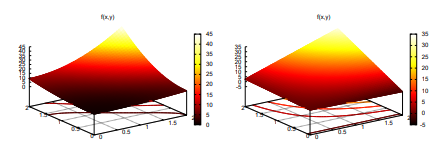
\includegraphics[width=0.7\linewidth]{img_33}
	\caption{Approximation of a 2D quadratic function (left) by a 2D bilinear
		function (right) using the Galerkin or least squares method.}
	\label{fig:img_33}
\end{figure}

\section[Implementation]{Implementation}
\label{sec:sec_8_3}
\noindent The least\textunderscore squares function from Section \hyperref[sec:sec_2_8]{2.8} and/or the file \href{https://github.com/hplgit/INF5620/blob/master/src/fem/fe_approx1D.py}{approx1D.py} can with very small modifications solve $2 \mathrm{D}$ approximation problems. First, let Omega now be a list of the intervals in $x$ and $y$ direction. For example, $\Omega=\left[0, L_{x}\right] \times\left[0, L_{y}\right]$ can be represented by Omega $=\left[\left[0, L_{-} \mathrm{x}\right],\left[0, \mathrm{~L}_{-} \mathrm{y}\right]\right]$. Second, the symbolic integration must be extended to $2 \mathrm{D}$ :
\begin{lstlisting}[numbers=none]
import sympy as sp

integrand = psi[i]*psi[j]
I = sp.integrate(integrand,

				(x, Omega[0][0], Omega[0][1]),
				(y, Omega[1][0], Omega[1][1]))	
\end{lstlisting}
provided integrand is an expression involving the sympy symbols x and y. The
2D version of numerical integration becomes
\begin{lstlisting}[numbers=none]
if isinstance(I, sp.Integral):
	integrand = sp.lambdify([x,y], integrand)
	I = sp.mpmath.quad(integrand,
						[Omega[0][0], Omega[0][1]],
						[Omega[1][0], Omega[1][1]])	
\end{lstlisting}
The right-hand side integrals are modified in a similar way.

Third, we must construct a list of $2 \mathrm{D}$ basis functions. Here are two examples based on tensor products of $1 \mathrm{D}$ "Taylor-style" polynomials $x^{i}$ and $1 \mathrm{D}$ sine functions $\sin ((i+1) \pi x)$ :
\begin{lstlisting}[numbers=none]
def taylor(x, y, Nx, Ny):
	return [x**i*y**j for i in range(Nx+1) for j in range(Ny+1)]
	
def sines(x, y, Nx, Ny):
	return [sp.sin(sp.pi*(i+1)*x)*sp.sin(sp.pi*(j+1)*y)
		for i in range(Nx+1) for j in range(Ny+1)]	
\end{lstlisting}
The complete code appears in \href{http://tinyurl.com/jvzzcfn/fem/fe_approx2D.py}{approx2D.py.}

The previous hand calculation where a quadratic f was approximated by a
bilinear function can be computed symbolically by
\begin{lstlisting}[numbers=none]
>>> from approx2D import *
>>> f = (1+x**2)*(1+2*y**2)
>>> psi = taylor(x, y, 1, 1)
>>> Omega = [[0, 2], [0, 2]]
>>> u = least_squares(f, psi, Omega)
>>> print u
8*x*y - 2*x/3 + 4*y/3 - 1/9
>>> print sp.expand(f)
2*x**2*y**2 + x**2 + 2*y**2 + 1	
\end{lstlisting}
We may continue with adding higher powers to the basis:
\begin{lstlisting}[numbers=none]
>>> psi = taylor(x, y, 2, 2)
>>> u = least_squares(f, psi, Omega)
>>> print u
2*x**2*y**2 + x**2 + 2*y**2 + 1
>>> print u-f
0	
\end{lstlisting}
For $N_{x} \geq 2$ and $N_{y} \geq 2$ we recover the exact function $f$, as expected, since in that case $f \in V$ (see Section \hyperref[sec:sec_2_5]{2.5}).
\bigbreak 

\section[Extension to 3D]{Extension to 3D}
\label{sec:sec_8_4}
\noindent Extension to 3D is in principle straightforward once the $2 \mathrm{D}$ extension is understood. The only major difference is that we need the repeated outer tensor product,
$$
V=V_{x} \otimes V_{y} \otimes V_{z}.
$$
In general, given vectors (first-order tensors) $a^{(q)}=\left(a_{0}^{(q)}, \ldots, a_{N_{q}}^{(q)}, q=0, \ldots, m\right.$, the tensor product $p=a^{(0)} \otimes \cdots \otimes a^{m}$ has elements
$$
p_{i_{0}, i_{1}, \ldots, i_{m}}=a_{i_{1}}^{(0)} a_{i_{1}}^{(1)} \cdots a_{i_{m}}^{(m)} .
$$
The basis functions in $3 \mathrm{D}$ are then
$$
\psi_{p, q, r}(x, y, z)=\hat{\psi}_{p}(x) \hat{\psi}_{q}(y) \hat{\psi}_{r}(z),
$$
with $p \in \mathcal{I}_{x}, q \in \mathcal{I}_{y}, r \in \mathcal{I}_{z}$. The expansion of $u$ becomes
$$
u(x, y, z)=\sum_{p \in \mathcal{I}_{x}} \sum_{q \in \mathcal{I}_{y}} \sum_{r \in \mathcal{I}_{z}} c_{p, q, r} \psi_{p, q, r}(x, y, z) .
$$
A single index can be introduced also here, e.g., $i=N_{x} N_{y} r+q_{N} x+p, u=$ $\sum_{i} c_{i} \psi_{i}(x, y, z)$.
\begin{mybox}
	\textbf{Use of tensor product spaces.}
	
	\noindent Constructing a multi-dimensional space and basis from tensor products of 1D spaces is a standard technique when working with global basis functions. In the world of finite elements, constructing basis functions by tensor products is much used on quadrilateral and hexahedra cell shapes, but not on triangles and tetrahedra. Also, the global finite element basis functions are almost exclusively denoted by a single index and not by the natural tuple of indices that arises from tensor products.
\end{mybox}

\chapter{Finite elements in 2D and 3D}
\label{chap:chap_9}
\noindent Finite element approximation is particularly powerful in $2 \mathrm{D}$ and 3D because the method can handle a geometrically complex domain $\Omega$ with ease. The principal idea is, as in $1 \mathrm{D}$, to divide the domain into cells and use polynomials for approximating a function over a cell. Two popular cell shapes are triangles and the quadrilaterals. Figures \hyperref[fig:img_34]{34}, \hyperref[fig:img_35]{35} , and \hyperref[fig:img_36]{36} provide examples. $\mathrm{P} 1$ elements means linear functions $\left(a_{0}+a_{1} x+a_{2} y\right)$ over triangles, while Q1 elements have bilinear functions $\left(a_{0}+a_{1} x+a_{2} y+a_{3} x y\right)$ over rectangular cells. Higher-order elements can easily be defined.
\begin{figure}[H]
	\centering
	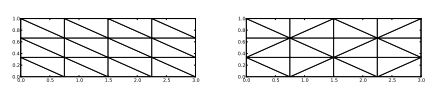
\includegraphics[width=0.7\linewidth]{img_34}
	\caption{Examples on 2D P1 elements.}
	\label{fig:img_34}
\end{figure}
\begin{figure}[H]
	\centering
	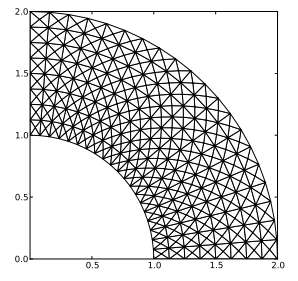
\includegraphics[width=0.7\linewidth]{img_35}
	\caption{Examples on 2D P1 elements in a deformed geometry.}
	\label{fig:img_35}
\end{figure}
\section[Basis functions over triangles in the physical domain]{Basis functions over triangles in the physical domain}
\label{sec:sec_9_1}
\noindent Cells with triangular shape will be in main focus here. With the $\mathrm{P} 1$ triangular element, $u$ is a linear function over each cell, as depicted in Figure \hyperref[fig:img_37]{37}, with discontinuous derivatives at the cell boundaries.

We give the vertices of the cells global and local numbers as in 1D. The degrees of freedom in the $\mathrm{P} 1$ element are the function values at a set of nodes, which are the three vertices. The basis function $\varphi_{i}(x, y)$ is then 1 at the vertex with global vertex number $i$ and zero at all other vertices. On an element, the three degrees of freedom uniquely determine the linear basis functions in that element, as usual. The global $\varphi_{i}(x, y)$ function is then a combination of the linear functions (planar surfaces) over all the neighboring cells that have vertex number $i$ in common. Figure \hyperref[fig:img_38]{38} tries to illustrate the shape of such a "pyramid"-like function.
\begin{figure}[H]
	\centering
	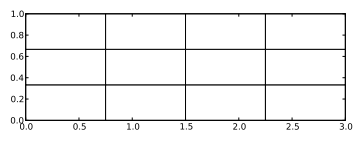
\includegraphics[width=0.7\linewidth]{img_36}
	\caption{Examples on 2D Q1 elements.}
	\label{fig:img_36}
\end{figure}

\noindent \textbf{Element matrices and vectors}. As in $1 \mathrm{D}$, we split the integral over $\Omega$ into a sum of integrals over cells. Also as in 1D, $\varphi_{i}$ overlaps $\varphi_{j}$ (i.e., $\varphi_{i} \varphi_{j} \neq 0$ ) if and only if $i$ and $j$ are vertices in the same cell. Therefore, the integral of $\varphi_{i} \varphi_{j}$ over an element is nonzero only when $i$ and $j$ run over the vertex numbers in the element. These nonzero contributions to the coefficient matrix are, as in 1D, collected in an element matrix. The size of the element matrix becomes $3 \times 3$ since there are three degrees of freedom that $i$ and $j$ run nver. Again, as in 1D, we number the local vertices in a cell, starting at 0 , and add the entries in the element matrix into the global system matrix, exactly as in 1D. All details and code appear below.
\bigbreak
\section[Basis functions over triangles in the reference cell]{Basis functions over triangles in the reference cell}
\label{sec:sec_9_2}
\noindent As in 1D, we can define the basis functions and the degrees of freedom in a reference cell and then use a mapping from the reference coordinate system to the physical coordinate system. We also have a mapping of local degrees of freedom numbers to global degrees of freedom numbers.

The reference cell in an $(X, Y)$ coordinate system has vertices $(0,0),(1,0)$, and $(0,1)$, corresponding to local vertex numbers 0,1 , and 2 , respectively. The $\mathrm{P} 1$ element has linear functions $\tilde{\varphi}_{r}(X, Y)$ as basis functions, $r=0,1,2$. Since a linear function $\tilde{\varphi}_{r}(X, Y)$ in $2 \mathrm{D}$ is on the form $C_{r, 0}+C_{r, 1} X+C_{r, 2} Y$, and hence has three parameters $C_{r, 0}, C_{r, 1}$, and $C_{r, 2}$, we need three degrees of freedom. These are in general taken as the function values at a set of nodes. For the P1
\begin{figure}[H]
	\centering
	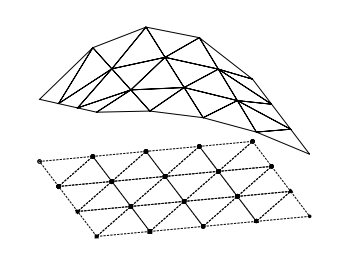
\includegraphics[width=0.7\linewidth]{img_37}
	\caption{Example on piecewise linear 2D functions defined on triangles.}
	\label{fig:img_37}
\end{figure}
\noindent element the set of nodes is the three vertices. Figure \hyperref[fig:img_39]{39} displays the geometry of the element and the location of the nodes.

Requiring $\tilde{\varphi}_{r}=1$ at node number $r$ and $\tilde{\varphi}_{r}=0$ at the two other nodes, gives three linear equations to determine $C_{r, 0}, C_{r, 1}$, and $C_{r, 2}$. The result is
\begin{equation}\label{eqa109}
	\tilde{\varphi}_{0}(X, Y)=1-X-Y,
\end{equation}
\begin{equation}\label{eqa110}
	\tilde{\varphi}_{1}(X, Y)=X,
\end{equation}
\begin{equation}\label{eqa111}
	\tilde{\varphi}_{2}(X, Y)=Y
\end{equation}
Higher-order approximations are obtained by increasing the polynomial order, adding additional nodes, and letting the degrees of freedom be function values at the nodes. Figure \hyperref[fig:img_40]{40} shows the location of the six nodes in the P2 element.
A polynomial of degree $p$ in $X$ and $Y$ has $n_{p}=(p+1)(p+2) / 2$ terms and hence needs $n_{p}$ nodes. The values at the nodes constitute $n_{p}$ degrees of freedom. The location of the nodes for $\tilde{\varphi}_{r}$ up to degree 6 is displayed in Figure \hyperref[fig:img_41]{41}.

The generalization to $3 \mathrm{D}$ is straightforward: the reference element is a \href{https://en.wikipedia.org/wiki/Tetrahedron}{tetrahedron} with vertices $(0,0,0),(1,0,0),(0,1,0)$, and $(0,0,1)$ in a $X, Y, Z$ reference coordinate system. The $\mathrm{P} 1$ element has its degrees of freedom as four nodes, which are the four vertices, see Figure \hyperref[fig:img_42]{42} . The $\mathrm{P} 2$ element adds additional nodes along the edges of the cell, yielding a total of 10 nodes and degrees of freedom, see Figure \hyperref[fig:img_43]{43} .

The interval in 1D, the triangle in 2D, the tetrahedron in 3D, and its generalizations to higher space dimensions are known as \textit{simplex} cells (the
\begin{figure}[H]
	\centering
	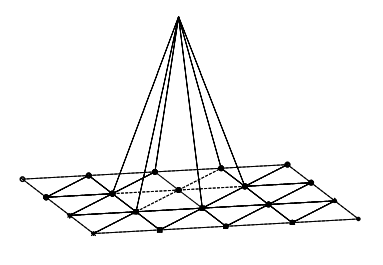
\includegraphics[width=0.7\linewidth]{img_38}
	\caption{Example on a piecewise linear 2D basis function over a patch of
		triangles.}
	\label{fig:img_38}
\end{figure}
\begin{figure}[H]
	\centering
	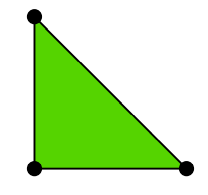
\includegraphics[width=0.7\linewidth]{img_39}
	\caption{2D P1 element.}
	\label{fig:img_39}
\end{figure}

\noindent geometry) or \textit{simplex} elements (the geometry, basis functions, degrees of freedom,
etc.). The plural forms \href{https://en.wikipedia.org/wiki/Simplex}{simplices} and simplexes are also a much used shorter
terms when referring to this type of cells or elements. The side of a simplex is
called a \textit{face}, while the tetrahedron also has \textit{edges}.

Acknowledgment. Figures \hyperref[fig:img_39]{39} to \hyperref[fig:img_43]{43} are created by Anders Logg and taken
from the \href{https://launchpad.net/fenics-book}{FEniCS book}: \textit{Automated Solution of Differential Equations by the
Finite Element Method}, edited by A. Logg, K.-A. Mardal, and G. N. Wells,
published by \href{https://link.springer.com/book/10.1007/978-3-642-23099-8}{Springer}, 2012.
\begin{figure}[H]
	\centering
	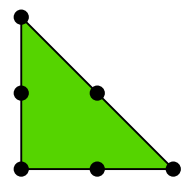
\includegraphics[width=0.7\linewidth]{img_40}
	\caption{2D P2 element.}
	\label{fig:img_40}
\end{figure}
\begin{figure}[H]
	\centering
	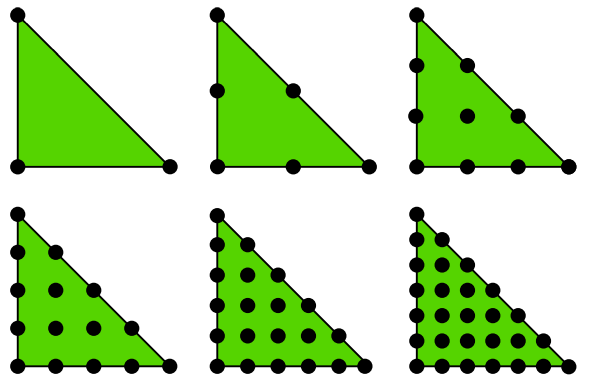
\includegraphics[width=0.7\linewidth]{img_41}
	\caption{2D P1, P2, P3, P4, P5, and P6 elements.}
	\label{fig:img_41}
\end{figure}
\section[Affine mapping of the reference cell]{Affine mapping of the reference cell}
\label{sec:sec_9_3}
\noindent Let $\tilde{\varphi}_{r}^{(1)}$ denote the basis functions associated with the $\mathrm{P} 1$ element in $1 \mathrm{D}, 2 \mathrm{D}$, or 3D, and let $\boldsymbol{x}_{q(e, r)}$ be the physical coordinates of local vertex number $r$ in cell $e$. Furthermore, let $\boldsymbol{X}$ be a point in the reference coordinate system corresponding to the point $\boldsymbol{x}$ in the physical coordinate system. The affine mapping of any $\boldsymbol{X}$ onto $\boldsymbol{x}$ is then defined by
\begin{equation}\label{eqa112}
	x=\sum_{r} \tilde{\varphi}_{r}^{(1)}(X) x_{q(e, r)},
\end{equation}
where $r$ runs over the local vertex numbers in the cell. The affine mapping essentially stretches, translates, and rotates the triangle. Straight or planar
\begin{figure}[H]
	\centering
	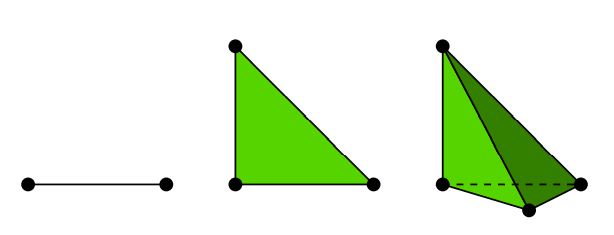
\includegraphics[width=0.7\linewidth]{img_42}
	\caption{P1 elements in 1D, 2D, and 3D.}
	\label{fig:img_42}
\end{figure}
\begin{figure}[H]
	\centering
	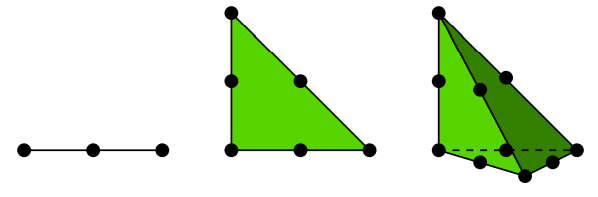
\includegraphics[width=0.7\linewidth]{img_43}
	\caption{P2 elements in 1D, 2D, and 3D.}
	\label{fig:img_43}
\end{figure}

\noindent faces of the reference cell are therefore mapped onto straight or planar faces
in the physical coordinate system. The mapping can be used for both P1 and
higher-order elements, but note that the mapping itself always applies the P1
basis functions.
\section[Isoparametric mapping of the reference cell]{Isoparametric mapping of the reference cell}
\label{sec:sec_9_4}
Instead of using the $\mathrm{P} 1$ basis functions in the mapping (\hyperref[eqa112]{112}), we may use the basis functions of the actual $\mathrm{Pd}$ element:
\begin{equation}\label{eqa113}
	x=\sum_{r} \tilde{\varphi}_{r}(X) x_{q(e, r)},
\end{equation}
where $r$ runs over all nodes, i.e., all points associated with the degrees of freedom. This is called an \textit{isoparametric mapping}. For P1 elements it is identical to the affine mapping (\hyperref[eqa112]{112}), but for higher-order elements the mapping of the straight or planar faces of the reference cell will result in a \textit{curved} face in the physical coordinate system. For example, when we use the basis functions of the triangular P2 element in $2 \mathrm{D}$ in (\hyperref[eqa113]{113}), the straight faces of the reference triangle are mapped onto curved faces of parabolic shape in the physical coordinate system, see Figure \hyperref[fig:img_45]{45} .
\begin{figure}[H]
	\centering
	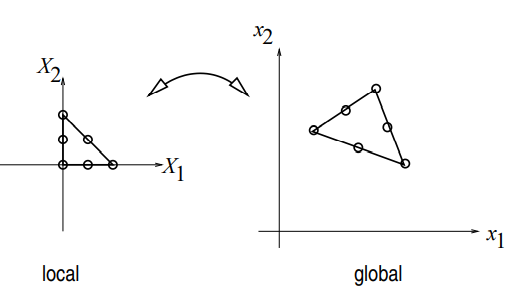
\includegraphics[width=0.7\linewidth]{img_44}
	\caption{Affine mapping of a P1 element.}
	\label{fig:img_44}
\end{figure}
\begin{figure}[H]
	\centering
	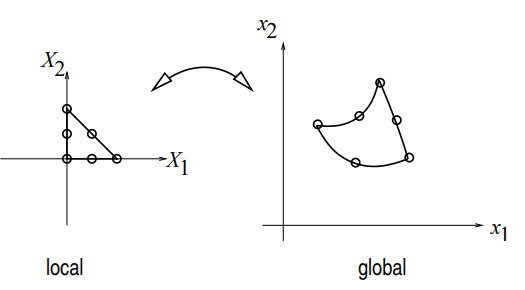
\includegraphics[width=0.7\linewidth]{img_45}
	\caption{Isoparametric mapping of a P2 element.}
	\label{fig:img_45}
\end{figure}

From (\hyperref[eqa112]{112}) or (\hyperref[eqa113]{113}) it is easy to realize that the vertices are correctly mapped. Consider a vertex with local number $s$. Then $\tilde{\varphi}_{s}=1$ at this vertex and zero at the others. This means that only one term in the sum is nonzero and $\boldsymbol{x}=\boldsymbol{x}_{q(e, s)}$, which is the coordinate of this vertex in the global coordinate system.
\section[Computing integrals]{Computing integrals}
\label{sec:sec_9_5}
Let $\tilde{\Omega}^{r}$ denote the reference cell and $\Omega^{(e)}$ the cell in the physical coordinate system. The transformation of the integral from the physical to the reference coordinate system reads
\begin{equation}\label{eqa114}
	\int_{\Omega^{(e)}} \varphi_{i}(\boldsymbol{x}) \varphi_{j}(\boldsymbol{x}) \mathrm{d} x =\int_{\tilde{\Omega}^{r}} \tilde{\varphi}_{i}(\boldsymbol{X}) \tilde{\varphi}_{j}(\boldsymbol{X}) \operatorname{det} J \mathrm{~d} X
\end{equation}
\begin{equation}\label{eqa115}
	\int_{\Omega^{(e)}} \varphi_{i}(\boldsymbol{x}) f(\boldsymbol{x}) \mathrm{d} x =\int_{\tilde{\Omega}^{r}} \tilde{\varphi}_{i}(\boldsymbol{X}) f(\boldsymbol{x}(\boldsymbol{X})) \operatorname{det} J \mathrm{~d} X
\end{equation}

\noindent where $\mathrm{d} x$ means the infinitesimal area element $d x d y$ in $2 \mathrm{D}$ and $d x d y d z$ in 3D, with a similar definition of $\mathrm{d} X$. The quantity det $J$ is the determinant of the Jacobian of the mapping $\boldsymbol{x}(\boldsymbol{X})$. In 2D,
\begin{equation}\label{eqa116}
	J=\left[\begin{array}{ll}
		\frac{\partial x}{\partial X} & \frac{\partial x}{\partial Y} \\
		\frac{\partial y}{\partial X} & \frac{\partial y}{\partial Y}
	\end{array}\right], \quad \operatorname{det} J=\frac{\partial x}{\partial X} \frac{\partial y}{\partial Y}-\frac{\partial x}{\partial Y} \frac{\partial y}{\partial X} .
\end{equation}
With the affine mapping (\hyperref[eqa112]{112}), $\operatorname{det} J=2 \Delta$, where $\Delta$ is the area or volume of the cell in the physical coordinate system.
\bigbreak
\noindent \textbf{Remark.} Observe that finite elements in 2D and 3D builds on the same ideas and \textit{concepts} as in $1 \mathrm{D}$, but there is simply much more to compute because the specific mathematical formulas in 2D and $3 \mathrm{D}$ are more complicated and the book keeping with dof maps also gets more complicated. The manual work is tedious, lengthy, and error-prone so automation by the computer is a must.
\chapter{Exercises}
\label{chap:chap_10}

\section*{Exercise 1: Linear algebra refresher I}
\label{sec:sec_10_1}
\noindent Look up the topic of \textit{vector} space in your favorite linear algebra book or search for the term at Wikipedia. Prove that vectors in the plane $(a, b)$ form a vector space by showing that all the axioms of a vector space are satisfied. Similarly, prove that all linear functions of the form $a x+b$ constitute a vector space, $a, b \in \mathbb{R}$.

On the contrary, show that all quadratic functions of the form $1+a x^{2}+b x$ \textit{do not} constitute a vector space. Filename: linalg1.pdf.
\bigbreak
\section*{Exercise 2: Linear algebra refresher II}
\label{sec:sec_10_2}
\noindent As an extension of Exercise 1, check out the topic of \textit{inner product spaces}. Suggest a possible inner product for the space of all linear functions of the form $a x+b$, $a, b \in \mathbb{R}$. Show that this inner product satisfies the general requirements of an inner product in a vector space. Filename: linalg2.pdf.
\bigbreak
\section*{Exercise 3: Approximate a three-dimensional vector in a plane}
\label{sec:sec_10_3}
\noindent Given $\boldsymbol{f}=(1,1,1)$ in $\mathbb{R}^{3}$, find the best approximation vector $\boldsymbol{u}$ in the plane spanned by the unit vectors $(1,0)$ and $(0,1)$. Repeat the calculations using the vectors $(2,1)$ and $(1,2)$. Filename: vec111\textunderscore approx.pdf.
\bigbreak
\section*{Exercise 4: Approximate the exponential function by power functions}
\label{sec:sec_10_4}
\noindent Let $V$ be a function space with basis functions $x^{i}, i=0,1, \ldots, N$. Find the best approximation to $f(x)=\exp (-x)$ on $\Omega=[0,4]$ among all functions in $V$ for $N=2,4,6$. Illustrate the three approximations in three separate plots. Add the corresponding Taylor polynomial approximation of degree $N$ in each plot. Filename: exp\textunderscore powers.py.
\bigbreak
\section*{Exercise 5: Approximate the sine function by power functions}
\label{sec:sec_10_5}
\noindent Let $V$ be a function space with basis functions $x^{2 i+1}, i=0,1, \ldots, N$. Find the best approximation to $f(x)=\sin (x)$ among all functions in $V$, using $N=8$ for a domain that includes more and more half-periods of the sine function: $\Omega=[0, k \pi / 2], k=2,3, \ldots, 12$. How does a Taylor series of $\sin (x)$ around $x$ up to degree 9 behave for the largest domain?
\bigbreak
\noindent \textbf{Hint.} One can make a loop over $k$ and call the functions least\textunderscore squares and comparison\textunderscore plot from the approx1D module.

Filename: sin\textunderscore powers.py.
\bigbreak
\section*{Exercise 6: Approximate a steep function by sines}
\label{sec:sec_10_6}
\noindent Find the best approximation of $f(x)=\tanh (s(x-\pi))$ on $[0,2 \pi]$ in the space $V$ with basis $\psi_{i}(x)=\sin ((2 i+1) x), i \in \mathcal{I}_{s}=\{0, \ldots, N\}$. Make a movie showing how $u=\sum_{j \in \mathcal{I}_{s}} c_{j} \psi_{j}(x)$ approximates $f(x)$ as $N$ grows. Choose $s$ such that $f$ is steep ( $s=20$ may be appropriate).
\bigbreak
\noindent \textbf{Hint.} One may naively call the least\textunderscore squares\textunderscore orth and comparison\textunderscore plot from the approx1D module in a loop and extend the basis with one new element in each pass. This approach implies a lot of recomputations. A more efficient strategy is to let least\textunderscore squares\textunderscore orth compute with only one basis function at a time and accumulate the corresponding $u$ in the total solution.
Filename: tanh\textunderscore sines\textunderscore approx1.py.
\bigbreak
\section*{Exercise 7: Animate the approximation of a steep function by sines}
\label{sec:sec_10_7}
\noindent Make a movie where the steepness $(s)$ of the tanh function in Exercise \hyperref[sec:sec_10_6]{6} grows in "time", and for each value of the steepness, the movie shows how the approximation improves with increasing $N$. Filename: tanh\textunderscore sines\textunderscore approx2.py.
\bigbreak
\section*{Exercise 8: Fourier series as a least squares approximation}
\label{sec:sec_10_8}
\noindent Given a function $f(x)$ on an interval $[0, L]$, look up the formula for the coefficients $a_{j}$ and $b_{j}$ in the Fourier series of $f$ :
$$
f(x)=a_{0}+\sum_{j=1}^{\infty} a_{j} \cos \left(j \frac{\pi x}{L}\right)+\sum_{j=1}^{\infty} b_{j} \sin \left(j \frac{\pi x}{L}\right).
$$
Let an infinite-dimensional vector space $V$ have the basis functions $\cos j \frac{\pi x}{L}$ for $j=0,1, \ldots, \infty$ and $\sin j \frac{\pi x}{L}$ for $j=1, \ldots, \infty$. Show that the least squares approximation method from Section \hyperref[chap:chap_2]{2} leads to a linear system whose solution coincides with the standard formulas for the coefficients in a Fourier series of $\int(x)$ (see also Section \hyperref[sec:sec_2_7]{2.7}). You may choose
$$
\psi_{2 i}=\cos \left(i \frac{\pi}{L} x\right), \quad \psi_{2 i+1}=\sin \left(i \frac{\pi}{L} x\right),
$$
for $i=0,1, \ldots, N \rightarrow \infty$.
Choose $f(x)=\tanh \left(s\left(x-\frac{1}{2}\right)\right)$ on $\Omega=[0,1]$, which is a smooth function, but with considerable steepness around $x=1 / 2$ as $s$ grows in size. Calculate the coefficients in the Fourier expansion by solving the linear system, arising from the least squares or Galerkin methods, by hand. Plot some truncated versions of the series together with $f(x)$ to show how the series expansion converges for $s=10$ and $s=100$. Filename: Fourier\textunderscore approx.py.
\bigbreak
\section*{Exercise 9: Approximate a steep function by Lagrange polynomials}
\label{sec:sec_10_9}
\noindent Use interpolation/collocation with uniformly distributed points and Chebychev nodes to approximate
$$
f(x)=-\tanh \left(s\left(x-\frac{1}{2}\right)\right), \quad x \in[0,1]
$$
by Lagrange polynomials for $s=10$ and $s=100$, and $N=3,6,9,11$. Make separate plots of the approximation for each combination of $s$, point type (Chebyshev or uniform), and $N$. Filename: tanh\textunderscore Lagrange.py.
\bigbreak
\section*{Exercise 10: Define nodes and elements}
\label{sec:sec_10_10}
\noindent Consider a domain $\Omega=[0,2]$ divided into the three $\mathrm{P} 2$ elements $[0,1],[1,1.2]$, and $[1.2,2]$.

For P1 and P2 elements, set up the list of coordinates and nodes (nodes) and the numbers of the nodes that belong to each element (elements) in two cases: 1) nodes and elements numbered from left to right, and 2) nodes and elements numbered from right to left. Filename: fe\textunderscore numberings 1 .py ..
\bigbreak
\section*{Exercise 11: Define vertices, cells, and dof maps}
\label{sec:sec_10_11}
\noindent Repeat Exercise \hyperref[sec:sec_10_10]{10}, but define the data structures vertices, cells, and dof\textunderscore map instead of nodes and elements. Filename: fe\textunderscore numberings2.py.
\bigbreak
\section*{Exercise 12: Construct matrix sparsity patterns}
\label{sec:sec_10_12}
\noindent Exercise \hyperref[sec:sec_10_10]{10} describes a element mesh with a total of five elements, but with two different element and node orderings. For each of the two orderings, make a $5 \times 5$ matrix and fill in the entries that will be nonzero.
\bigbreak
\noindent \textbf{Hint.} A matrix entry $(i, j)$ is nonzero if $i$ and $j$ are nodes in the same element. Filename: \textunderscore sparsity\textunderscore pattern.pdf.

\section*{Exercise 13: Perform symbolic finite element computations}
\label{sec:sec_10_13}
\noindent Perform hand calculations to find formulas for the coefficient matrix and righthand side when approximating $f(x)=\sin (x)$ on $\Omega=[0, \pi]$ by two P1 elements of size $\pi / 2$. Solve the system and compare $u(\pi / 2)$ with the exact value 1 .
Filename: sin\textunderscore approx\textunderscore P1.py.
\bigbreak
\section*{Exercise 14: Approximate a steep function by $\mathrm{P} 1$ and $\mathrm{P} 2$ elements}
\label{sec:sec_10_14}
\noindent Given
$$
f(x)=\tanh \left(s\left(x-\frac{1}{2}\right)\right)
$$
use the Galerkin or least squares method with finite elements to find an approximate function $u(x)$. Choose $s=40$ and try $N_{e}=4,8,16 \mathrm{P} 1$ elements and $N_{e}=2,4,8 \mathrm{P} 2$ elements. Integrate $f \varphi_{i}$ numerically. Filename: tanh\textunderscore fe\textunderscore P1P2\textunderscore approx.py.
\bigbreak
\section*{Exercise 15: Approximate a steep function by $\mathrm{P} 3$ and $\mathrm{P} 4$ elements}
\label{sec:sec_10_15}
\noindent Solve Exercise \hyperref[sec:sec_10_14]{14} using $N_{e}=1,2,4 \mathrm{P} 3$ and P4 elements. How will a collocation/interpolation method work in this case with the same number of nodes? Filename: tanh\textunderscore fe\textunderscore P3P4\textunderscore approx.py.
\bigbreak
\section*{Exercise 16: Investigate the approximation error in finite elements}
\label{sec:sec_10_16}
\noindent The theory (\hyperref[eqa93]{93}) from Section ?? predicts that the error in the $\mathrm{P} d$ approximation of a function should behave as $h^{d+1}$. Use experiments to verify this asymptotic behavior (i.e., for small enough $h$ ). Choose two examples: $f(x)=A e^{-\omega x}$ on

$[0,3 / \omega]$ and $f(x)=A \sin (\omega x)$ on $\Omega=[0,2 \pi / \omega]$ for constants $A$ and $\omega$. What happens if you try $f(x)=\sqrt{x}$ on $[0,1]$ ?
\bigbreak
\noindent \textbf{Hint}. Run a series of experiments: $\left(h_{i}, E\right), i=0, \ldots, m$, where $E_{i}$ is the $L^{2}$ norm of the error corresponding to element length $h_{i}$. Assume an error model $E=C h^{r}$ and compute $r$ from two successive experiments:
$$
r_{i}=\ln \left(E_{i+1} / E_{i}\right) / \ln \left(h_{i+1} / h_{i}\right), \quad i=0, \ldots, m-1 .
$$
Hopefully, the sequence $r_{0}, \ldots, r_{m-1}$ converges to the true $r$, and $r_{m-1}$ can be taken as an approximation to $r$.

Filename: Asinwt\textunderscore interpolation\textunderscore error.py.
\bigbreak
\section*{Exercise 17: Approximate a step function by finite elements}
\label{sec:sec_10_17}
\noindent Approximate the step function
$$
f(x)= \begin{cases}1 & x<1 / 2 \\ 2 & x \geq 1 / 2\end{cases}
$$
by 2,4 , and $8 \mathrm{P} 1$ and P2 elements. Compare approximations visually.
Hint. This $f$ can also be expressed in terms of the Heaviside function $H(x)$ : $f(x)=H(x-1 / 2)$. Therefore, $f$ can be defined by
\begin{lstlisting}[numbers=none]
f = sp.Heaviside(x - sp.Rational(1,2))	
\end{lstlisting}
making the approximate function in the fe\textunderscore approx1D.py module an obvious candidate to solve the problem. However, sympy does not handle symbolic integration with this particular integrand, and the approximate function faces a problem when converting $f$ to a Python function (for plotting) since Heaviside is not an available function in numpy. It is better to make special-purpose code for this case or perform all calculations by hand.

Filename: Heaviside\textunderscore approx\textunderscore P1P2.py ..
\bigbreak
\section*{Exercise 18: 2D approximation with orthogonal functions}
\label{sec:sec_10_18}
\noindent Assume we have basis functions $\varphi_{i}(x, y)$ in $2 \mathrm{D}$ that are orthogonal such that $\left(\varphi_{i}, \varphi_{j}\right)=0$ when $i \neq j$. The function least\textunderscore squares in the file \href{http://tinyurl.com/jvzzcfn/fem/fe_approx2D.py}{approx2D.py} will then spend much time on computing off-diagonal terms in the coefficient matrix that we know are zero. To speed up the computations, make a version least\textunderscore squares\textunderscore orth that utilizes the orthogonality among the basis functions. Apply the function to approximate
$$
f(x, y)=x(1-x) y(1-y) e^{-x-y}
$$
on $\Omega=[0,1] \times[0,1]$ via basis functions
$$
\varphi_{i}(x, y)=\sin (p \pi x) \sin (q \pi y), \quad i=q N_{x}+p
$$

\noindent \textbf{Hint.} Get ideas from the function least\textunderscore squares\textunderscore orth in Section 2.8 and
file \href{http://tinyurl.com/jvzzcfn/fem/fe_approx2D.py}{approx2D.py.}

Filename: approx2D\textunderscore lsorth\textunderscore sin.py.
\bigbreak
\section*{Exercise 19: Use the Trapezoidal rule and $\mathrm{P} 1$ elements}
\label{sec:sec_10_19}
\noindent Consider approximation of some $f(x)$ on an interval $\Omega$ using the least squares or Galerkin methods with $\mathrm{P} 1$ elements. Derive the element matrix and vector using the Trapezoidal rule (\hyperref[eqa101]{101}) for calculating integrals on the reference element. Assemble the contributions, assuming a uniform cell partitioning, and show that the resulting linear system has the form $c_{i}=f\left(x_{i}\right)$ for $i \in \mathcal{I}_{s}$. Filename: fe\textunderscore P1\textunderscore trapez.pdf.
\bigbreak
\section*{Problem 20: Compare P1 elements and interpolation}
\label{sec:sec_10_20}
\noindent We shall approximate the function
$$
f(x)=1+\epsilon \sin (2 \pi n x), \quad x \in \Omega=[0,1]
$$
where $n \in \mathbb{Z}$ and $\epsilon \geq 0$.
\begin{enumerate}[label=(\alph*)]
	\item Sketch $f(x)$ and find the wave length of the function.
	\item We want to use $N_{P}$ elements per wave length. Show that the number of elements is then $n N_{P}$.
	\item The critical quantity for accuracy is the number of elements per wave length, not the element size in itself. It therefore suffices to study an $f$ with just one wave length in $\Omega=[0,1]$. Set $\epsilon=0.5$.
	
	Run the least squares or projection/Galerkin method for $N_{P}=2,4,8,16,32$. Compute the error $E=\|u-f\|_{L^{2}}$.
	\bigbreak
	\textbf{Hint.} Use the fe\textunderscore approx1D\textunderscore numint module to compute $u$ and use the technique from Section \hyperref[sec:sec_6_4]{6.4} to compute the norm of the error.
	\item Repeat the set of experiments in the above point, but use interpolation/collocation based on the node points to compute $u(x)$ (recall that $c_{i}$ is now simply $\left.f\left(x_{i}\right)\right)$. Compute the error $E=\|u-f\|_{L^{2}}$. Which method seems to be most accurate?
	
	Filename: P1\textunderscore vs\textunderscore interp.py.
\end{enumerate}
\bigbreak
\section*{Exercise 21: Implement 3D computations with global basis functions}
\label{sec:sec_10_21}
\noindent Extend the \href{http://tinyurl.com/jvzzcfn/fem/approx2D.py}{approx2D.py} code to 3D applying ideas from Section \hyperref[sec:sec_8_4]{8.4}. Use a
3D generalization of the test problem in Section \hyperref[sec:sec_8_3]{8.3} to test the implementation.
Filename: approx3D.py
\bigbreak
\section*{Exercise 22: Use Simpson's rule and P2 elements}
\label{sec:sec_10_22}
\noindent Redo Exercise \hyperref[sec:sec_10_19]{19}, but use P2 elements and Simpson's rule based on sampling
the integrands at the nodes in the reference cell.
Filename: fe\textunderscore P2\textunderscore simpson.pdf.

\end{document} 
